\documentclass[output=paper]{../langscibook}
\ChapterDOI{10.5281/zenodo.10185948}
\title{Coordination}
\author{Agnieszka Patejuk\affiliation{Polish Academy of Sciences and University of Oxford}}
\abstract{Coordination is a rich and complex topic. To avoid repeating what has been written in many excellent textbooks and reference guides, this chapter takes a non-standard approach. It starts by presenting the very basics of coordination in LFG, it provides pointers to agreement phenomena related to coordination, and then it proceeds to discuss selected less well-known coordination phenomena and their treatment in LFG, including: non-constituent coordination, coordination of unlike categories, coordination of unlike grammatical functions and coordination involving ellipsis.}

\IfFileExists{../localcommands.tex}{
   \addbibresource{../localbibliography.bib}
   \addbibresource{thisvolume.bib}
   % add all extra packages you need to load to this file

\usepackage{tabularx}
\usepackage{multicol}
\usepackage{url}
\urlstyle{same}
%\usepackage{amsmath,amssymb}

% Tight underlining according to https://alexwlchan.net/2017/10/latex-underlines/
\usepackage{contour}
\usepackage[normalem]{ulem}
\renewcommand{\ULdepth}{1.8pt}
\contourlength{0.8pt}
\newcommand{\tightuline}[1]{%
  \uline{\phantom{#1}}%
  \llap{\contour{white}{#1}}}
  
\usepackage{listings}
\lstset{basicstyle=\ttfamily,tabsize=2,breaklines=true}

% \usepackage{langsci-basic}
\usepackage{langsci-optional}
\usepackage[danger]{langsci-lgr}
\usepackage{langsci-gb4e}
%\usepackage{langsci-linguex}
%\usepackage{langsci-forest-setup}
\usepackage[tikz]{langsci-avm} % added tikz flag, 29 July 21
% \usepackage{langsci-textipa}

\usepackage[linguistics,edges]{forest}
\usepackage{tikz-qtree}
\usetikzlibrary{positioning, tikzmark, arrows.meta, calc, matrix, shapes.symbols}
\usetikzlibrary{arrows, arrows.meta, shapes, chains, decorations.text}

%%%%%%%%%%%%%%%%%%%%% Packages for all chapters

% arrows and lines between structures
\usepackage{pst-node}

% lfg attributes and values, lines (relies on pst-node), lexical entries, phrase structure rules
\usepackage{packages/lfg-abbrevs}

% subfigures
\usepackage{subcaption}

% macros for small illustrations in the glossary
\usepackage{./packages/picins}

%%%%%%%%%%%%%%%%%%%%% Packages from contributors

% % Simpler Syntax packages
\usepackage{bm}
\tikzstyle{block} = [rectangle, draw, text width=5em, text centered, minimum height=3em]
\tikzstyle{line} = [draw, thick, -latex']

% Dependency packages
\usepackage{tikz-dependency}
%\usepackage{sdrt}

\usepackage{soul}

\usepackage[notipa]{ot-tableau}

% Historical
\usepackage{stackengine}
\usepackage{bigdelim}

% Morphology
\usepackage{./packages/prooftree}
\usepackage{arydshln}
\usepackage{stmaryrd}

% TAG
\usepackage{pbox}

\usepackage{langsci-branding}

   % %%%%%%%%% lang sci press commands

\newcommand*{\orcid}{}

\makeatletter
\let\thetitle\@title
\let\theauthor\@author
\makeatother

\newcommand{\togglepaper}[1][0]{
   \bibliography{../localbibliography}
   \papernote{\scriptsize\normalfont
     \theauthor.
     \titleTemp.
     To appear in:
     Dalrymple, Mary (ed.).
     Handbook of Lexical Functional Grammar.
     Berlin: Language Science Press. [preliminary page numbering]
   }
   \pagenumbering{roman}
   \setcounter{chapter}{#1}
   \addtocounter{chapter}{-1}
}

\DeclareOldFontCommand{\rm}{\normalfont\rmfamily}{\mathrm}
\DeclareOldFontCommand{\sf}{\normalfont\sffamily}{\mathsf}
\DeclareOldFontCommand{\tt}{\normalfont\ttfamily}{\mathtt}
\DeclareOldFontCommand{\bf}{\normalfont\bfseries}{\mathbf}
\DeclareOldFontCommand{\it}{\normalfont\itshape}{\mathit}
\makeatletter
\DeclareOldFontCommand{\sc}{\normalfont\scshape}{\@nomath\sc}
\makeatother

% Bug fix, 3 April 2021
\SetupAffiliations{output in groups = false,
                   separator between two = {\bigskip\\},
                   separator between multiple = {\bigskip\\},
                   separator between final two = {\bigskip\\}
                   }

% commands for all chapters
\setmathfont{LibertinusMath-Additions.otf}[range="22B8]

% punctuation between a sequence of years in a citation
% OLD: \renewcommand{\compcitedelim}{\multicitedelim}
\renewcommand{\compcitedelim}{\addcomma\space}

% \citegen with no parentheses around year
\providecommand{\citegenalt}[2][]{\citeauthor{#2}'s \citeyear*[#1]{#2}}

% avms with plain font, using langsci-avm package
\avmdefinestyle{plain}{attributes=\normalfont,values=\normalfont,types=\normalfont,extraskip=0.2em}
% avms with attributes and values in small caps, using langsci-avm package
\avmdefinestyle{fstr}{attributes=\scshape,values=\scshape,extraskip=0.2em}
% avms with attributes in small caps, values in plain font (from peter sells)
\avmdefinestyle{fstr-ps}{attributes=\scshape,values=\normalfont,extraskip=0.2em}

% reference to previous or following examples, from Stefan
%(\mex{1}) is like \next, referring to the next example
%(\mex{0}) is like \last, referring to the previous example, etc
\makeatletter
\newcommand{\mex}[1]{\the\numexpr\c@equation+#1\relax}
\makeatother

% do not add xspace before these
\xspaceaddexceptions{1234=|*\}\restrict\,}

% Several chapters use evnup -- this is verbatim from lingmacros.sty
\makeatletter
\def\evnup{\@ifnextchar[{\@evnup}{\@evnup[0pt]}}
\def\@evnup[#1]#2{\setbox1=\hbox{#2}%
\dimen1=\ht1 \advance\dimen1 by -.5\baselineskip%
\advance\dimen1 by -#1%
\leavevmode\lower\dimen1\box1}
\makeatother

% Centered entries in tables.  Requires array package.
\newcolumntype{P}[1]{>{\centering\arraybackslash}p{#1}}

% Reference to multiple figures, requested by Victoria Rosen
\newcommand{\figsref}[2]{Figures~\ref{#1}~and~\ref{#2}}
\newcommand{\figsrefthree}[3]{Figures~\ref{#1},~\ref{#2}~and~\ref{#3}}
\newcommand{\figsreffour}[4]{Figures~\ref{#1},~\ref{#2},~\ref{#3}~and~\ref{#4}}
\newcommand{\figsreffive}[5]{Figures~\ref{#1},~\ref{#2},~\ref{#3},~\ref{#4}~and~\ref{#5}}

% Semitic chapter:
\providecommand{\textchi}{χ}

% Prosody chapter
\makeatletter
\providecommand{\leftleadsto}{%
  \mathrel{\mathpalette\reflect@squig\relax}%
}
\newcommand{\reflect@squig}[2]{%
  \reflectbox{$\m@th#1$$\leadsto$}%
}
\makeatother
\newcommand\myrotaL[1]{\mathrel{\rotatebox[origin=c]{#1}{$\leadsto$}}}
\newcommand\Prosleftarrow{\myrotaL{-135}}
\newcommand\myrotaR[1]{\mathrel{\rotatebox[origin=c]{#1}{$\leftleadsto$}}}
\newcommand\Prosrightarrow{\myrotaR{135}}

% Core Concepts chapter
\newcommand{\anterm}[2]{#1\\#2}
\newcommand{\annode}[2]{#1\\#2}

% HPSG chapter
\newcommand{\HPSGphon}[1]{〈#1〉}
% for defining RSRL relations:
\newcommand{\HPSGsfl}{\enskip\ensuremath{\stackrel{\forall{}}{\Longleftarrow{}}}\enskip}
% AVM commands, valid only inside \avm{}
\avmdefinecommand {phon}[phon] { attributes=\itshape } % define a new \phon command
% Forest Set-up
\forestset
  {notin label above/.style={edge label={node[midway,sloped,above,inner sep=0pt]{\strut$\ni$}}},
    notin label below/.style={edge label={node[midway,sloped,below,inner sep=0pt]{\strut$\ni$}}},
  }

% Dependency chapter
\newcommand{\ua}{\ensuremath{\uparrow}}
\newcommand{\da}{\ensuremath{\downarrow}}
\forestset{
  dg edges/.style={for tree={parent anchor=south, child anchor=north,align=center,base=bottom},
                 where n children=0{tier=word,edge=dotted,calign with current edge}{}
                },
dg transfer/.style={edge path={\noexpand\path[\forestoption{edge}, rounded corners=3pt]
    % the line downwards
    (!u.parent anchor)-- +($(0,-l)-(0,4pt)$)-- +($(12pt,-l)-(0,4pt)$)
    % the horizontal line
    ($(!p.north west)+(0,l)-(0,20pt)$)--($(.north east)+(0,l)-(0,20pt)$)\forestoption{edge label};},!p.edge'={}},
% for Tesniere-style junctions
dg junction/.style={no edge, tikz+={\draw (!p.east)--(!.west) (.east)--(!n.west);}    }
}


% Glossary
\makeatletter % does not work with \newcommand
\def\namedlabel#1#2{\begingroup
   \def\@currentlabel{#2}%
   \phantomsection\label{#1}\endgroup
}
\makeatother


\renewcommand{\textopeno}{ɔ}
\providecommand{\textepsilon}{ɛ}

\renewcommand{\textbari}{ɨ}
\renewcommand{\textbaru}{ʉ}
\newcommand{\acutetextbari}{í̵}
\renewcommand{\textlyoghlig}{ɮ}
\renewcommand{\textdyoghlig}{ʤ}
\renewcommand{\textschwa}{ə}
\renewcommand{\textprimstress}{ˈ}
\newcommand{\texteng}{ŋ}
\renewcommand{\textbeltl}{ɬ}
\newcommand{\textramshorns}{ɤ}

\newbool{bookcompile}
\booltrue{bookcompile}
\newcommand{\bookorchapter}[2]{\ifbool{bookcompile}{#1}{#2}}




\renewcommand{\textsci}{ɪ}
\renewcommand{\textturnscripta}{ɒ}

\renewcommand{\textscripta}{ɑ}
\renewcommand{\textteshlig}{ʧ}
\providecommand{\textupsilon}{υ}
\renewcommand{\textyogh}{ʒ}
\newcommand{\textpolhook}{̨}

\renewcommand{\sectref}[1]{Section~\ref{#1}}

%\KOMAoptions{chapterprefix=true}

\renewcommand{\textturnv}{ʌ}
\renewcommand{\textrevepsilon}{ɜ}
\renewcommand{\textsecstress}{ˌ}
\renewcommand{\textscriptv}{ʋ}
\renewcommand{\textglotstop}{ʔ}
\renewcommand{\textrevglotstop}{ʕ}
%\newcommand{\textcrh}{ħ}
\renewcommand{\textesh}{ʃ}

% label for submitted and published chapters
\newcommand{\submitted}{{\color{red}Final version submitted to Language Science Press.}}
\newcommand{\published}{{\color{red}Final version published by
    Language Science Press, available at \url{https://langsci-press.org/catalog/book/312}.}}

% Treebank definitions
\definecolor{tomato}{rgb}{0.9,0,0}
\definecolor{kelly}{rgb}{0,0.65,0}

% Minimalism chapter
\newcommand\tr[1]{$<$\textcolor{gray}{#1}$>$}
\newcommand\gapline{\lower.1ex\hbox to 1.2em{\bf \ \hrulefill\ }}
\newcommand\cnom{{\llap{[}}Case:Nom{\rlap{]}}}
\newcommand\cacc{{\llap{[}}Case:Acc{\rlap{]}}}
\newcommand\tpres{{\llap{[}}Tns:Pres{\rlap{]}}}
\newcommand\fstackwe{{\llap{[}}Tns:Pres{\rlap{]}}\\{\llap{[}}Pers:1{\rlap{]}}\\{\llap{[}}Num:Pl{\rlap{]}}}
\newcommand\fstackone{{\llap{[}}Tns:Past{\rlap{]}}\\{\llap{[}}Pers:\ {\rlap{]}}\\{\llap{[}}Num:\ {\rlap{]}}}
\newcommand\fstacktwo{{\llap{[}}Pers:3{\rlap{]}}\\{\llap{[}}Num:Pl{\rlap{]}}\\{\llap{[}}Case:\ {\rlap{]}}}
\newcommand\fstackthr{{\llap{[}}Tns:Past{\rlap{]}}\\{\llap{[}}Pers:3{\rlap{]}}\\{\llap{[}}Num:Pl{\rlap{]}}} 
\newcommand\fstackfou{{\llap{[}}Pers:3{\rlap{]}}\\{\llap{[}}Num:Pl{\rlap{]}}\\{\llap{[}}Case:Nom{\rlap{]}}}
\newcommand\fstackonefill{{\llap{[}}Tns:Past{\rlap{]}}\\{\llap{[}}Pers:3{\rlap{]}}\\%
  {\llap{[}}Num:Pl{\rlap{]}}}
\newcommand\fstackoneint%
    {{\llap{[}}{\bf Tns:Past}{\rlap{]}}\\{\llap{[}}Pers:\ {\rlap{]}}\\{\llap{[}}Num:\ {\rlap{]}}}
\newcommand\fstacktwoint%
    {{\llap{[}}{\bf Pers:3}{\rlap{]}}\\{\llap{[}}{\bf Num:Pl}{\rlap{]}}\\{\llap{[}}Case:\ {\rlap{]}}}
\newcommand\fstackthrchk%
    {{\llap{[}}{\bf Tns:Past}{\rlap{]}}\\{\llap{[}}{Pers:3}{\rlap{]}}\\%
      {\llap{[}}Num:Pl{\rlap{]}}} 
\newcommand\fstackfouchk%
    {{\llap{[}}{\bf Pers:3}{\rlap{]}}\\{\llap{[}}{\bf Num:Pl}{\rlap{]}}\\%
      {\llap{[}}Case:Nom{\rlap{]}}}
\newcommand\uinfl{{\llap{[}}Infl:\ \ {\rlap{]}}}
\newcommand\inflpass{{\llap{[}}Infl:Pass{\rlap{]}}}
\newcommand\fepp{{\llap{[}}EPP{\rlap{]}}}
\newcommand\sepp{{\llap{[}}\st{EPP}{\rlap{]}}}
\newcommand\rdash{\rlap{\hbox to 24em{\hfill (dashed lines represent
      information flow)}}}


% Computational chapter
\usepackage{./packages/kaplan}
\renewcommand{\red}{\color{lsLightWine}}

% Sinitic
\newcommand{\FRAME}{\textsc{frame}\xspace}
\newcommand{\arglistit}[1]{{\textlangle}\textit{#1}{\textrangle}}

%WestGermanic
\newcommand{\streep}[1]{\mbox{\rule{1pt}{0pt}\rule[.5ex]{#1}{.5pt}\rule{-1pt}{0pt}\rule{-#1}{0pt}}}

\newcommand{\hspaceThis}[1]{\hphantom{#1}}


\newcommand{\FIG}{\textsc{figure}}
\newcommand{\GR}{\textsc{ground}}

%%%%% Morphology
% Single quote
\newcommand{\asquote}[1]{`{#1}'} % Single quotes
\newcommand{\atrns}[1]{\asquote{#1}} % Translation
\newcommand{\attrns}[1]{(\asquote{#1})} % Translation
\newcommand{\ascare}[1]{\asquote{#1}} % Scare quotes
\newcommand{\aqterm}[1]{\asquote{#1}} % Quoted terms
% Double quote
\newcommand{\adquote}[1]{``{#1}''} % Double quotes
\newcommand{\aquoot}[1]{\adquote{#1}} % Quotes
% Italics
\newcommand{\aword}[1]{\textit{#1}}  % mention of word
\newcommand{\aterm}[1]{\textit{#1}}
% Small caps
\newcommand{\amg}[1]{{\textsc{\MakeLowercase{#1}}}}
\newcommand{\ali}[1]{\MakeLowercase{\textsc{#1}}}
\newcommand{\feat}[1]{{\textsc{#1}}}
\newcommand{\val}[1]{\textsc{#1}}
\newcommand{\pred}[1]{\textsc{#1}}
\newcommand{\predvall}[1]{\textsc{#1}}
% Misc commands
\newcommand{\exrr}[2][]{(\ref{ex:#2}{#1})}
\newcommand{\csn}[3][t]{\begin{tabular}[#1]{@{\strut}c@{\strut}}#2\\#3\end{tabular}}
\newcommand{\sem}[2][]{\ensuremath{\left\llbracket \mbox{#2} \right\rrbracket^{#1}}}
\newcommand{\apf}[2][\ensuremath{\sigma}]{\ensuremath{\langle}#2,#1\ensuremath{\rangle}}
\newcommand{\formula}[2][t]{\ensuremath{\begin{array}[#1]{@{\strut}l@{\strut}}#2%
                                         \end{array}}}
\newcommand{\Down}{$\downarrow$}
\newcommand{\Up}{$\uparrow$}
\newcommand{\updown}{$\uparrow=\downarrow$}
\newcommand{\upsigb}{\mbox{\ensuremath{\uparrow\hspace{-0.35em}_\sigma}}}
\newcommand{\lrfg}{L\textsubscript{R}FG} 
\newcommand{\dmroot}{\ensuremath{\sqrt{\hspace{1em}}}}
\newcommand{\amother}{\mbox{\ensuremath{\hat{\raisebox{-.25ex}{\ensuremath{\ast}}}}}}
\newcommand{\expone}{\ensuremath{\xrightarrow{\nu}}}
\newcommand{\sig}{\mbox{$_\sigma\,$}}
\newcommand{\aset}[1]{\{#1\}}
\newcommand{\linimp}{\mbox{\ensuremath{\,\multimap\,}}}
\newcommand{\fsfunc}{\ensuremath{\Phi}\hspace*{-.15em}}
\newcommand{\cons}[1]{\ensuremath{\mbox{\textbf{\textup{#1}}}}}
\newcommand{\amic}[1][]{\cons{MostInformative$_c$}{#1}}
\newcommand{\amif}[1][]{\cons{MostInformative$_f$}{#1}}
\newcommand{\amis}[1][]{\cons{MostInformative$_s$}{#1}}
\newcommand{\amsp}[1][]{\cons{MostSpecific}{#1}}

%Glue
\newcommand{\glues}{Glue Semantics} % macro for consistency
\newcommand{\glue}{Glue} % macro for consistency
\newcommand{\lfgglue}{LFG$+$Glue} 
\newcommand{\scare}[1]{`{#1}'} % Scare quotes
\newcommand{\word}[1]{\textit{#1}}  % mention of word
\newcommand{\dquote}[1]{``{#1}''} % Double quotes
\newcommand{\high}[1]{\textit{#1}} % highlight (italicize)
\newcommand{\laml}{{L}} 
% Left interpretation double bracket
\newcommand{\Lsem}{\ensuremath{\left\llbracket}} 
% Right interpretation double bracket
\newcommand{\Rsem}{\ensuremath{\right\rrbracket}} 
\newcommand{\nohigh}[1]{{#1}} % nohighlight (regular font)
% Linear implication elimination
\newcommand{\linimpE}{\mbox{\small\ensuremath{\multimap_{\mathcal{E}}}}}
% Linear implication introduction, plain
\newcommand{\linimpI}{\mbox{\small\ensuremath{\multimap_{\mathcal{I}}}}}
% Linear implication introduction, with flag
\newcommand{\linimpIi}[1]{\mbox{\small\ensuremath{\multimap_{{\mathcal{I}},#1}}}}
% Linear universal elimination
\newcommand{\forallE}{\mbox{\small\ensuremath{\forall_{{\mathcal{E}}}}}}
% Tensor elimination
\newcommand{\tensorEij}[2]{\mbox{\small\ensuremath{\otimes_{{\mathcal{E}},#1,#2}}}}
% CG forward slash
\newcommand{\fs}{\ensuremath{/}} 
% s-structure mapping, no space after                                     
\newcommand{\sigb}{\mbox{$_\sigma$}}
% uparrow with s-structure mapping, with small space after  
\newcommand{\upsig}{\mbox{\ensuremath{\uparrow\hspace{-0.35em}_\sigma\,}}}
\newcommand{\fsa}[1]{\textit{#1}}
\newcommand{\sqz}[1]{#1}
% Angled brackets (types, etc.)
\newcommand{\bracket}[1]{\ensuremath{\left\langle\mbox{\textit{#1}}\right\rangle}}
% glue logic string term
\newcommand{\gterm}[1]{\ensuremath{\mbox{\textup{\textit{#1}}}}}
% abstract grammatical formative
\newcommand{\gform}[1]{\ensuremath{\mbox{\textsc{\textup{#1}}}}}
% let
\newcommand{\llet}[3]{\ensuremath{\mbox{\textsf{let}}~{#1}~\mbox{\textsf{be}}~{#2}~\mbox{\textsf{in}}~{#3}}}
% Word-adorned proof steps
\providecommand{\vformula}[2]{%
  \begin{array}[b]{l}
    \mbox{\textbf{\textit{#1}}}\\%[-0.5ex]
    \formula{#2}
  \end{array}
}

%TAG
\newcommand{\fm}[1]{\textsc{#1}}
\newcommand{\struc}[1]{{#1-struc\-ture}}
\newcommand{\func}[1]{\mbox{#1-function}}
\newcommand{\fstruc}{\struc{f}}
\newcommand{\cstruc}{\struc{c}}
\newcommand{\sstruc}{\struc{s}}
\newcommand{\astruc}{\struc{a}}
\newcommand{\nodelabels}[2]{\rlap{\ensuremath{^{#1}_{#2}}}}
\newcommand{\footnode}{\rlap{\ensuremath{^{*}}}}
\newcommand{\nafootnode}{\rlap{\ensuremath{^{*}_{\nalabel}}}}
\newcommand{\nanode}{\rlap{\ensuremath{_{\nalabel}}}}
\newcommand{\AdjConstrText}[1]{\textnormal{\small #1}}
\newcommand{\nalabel}{\AdjConstrText{NA}}

%Case
\newcommand{\MID}{\textsc{mid}{}\xspace}

%font commands added April 2023 for Control and Case chapters
\def\textthorn{þ}
\def\texteth{ð}
\def\textinvscr{ʁ}
\def\textcrh{ħ}
\def\textgamma{ɣ}

% Coordination
\newcommand{\CONJ}{\textsc{conj}{}\xspace}
\newcommand*{\phtm}[1]{\setbox0=\hbox{#1}\hspace{\wd0}}
\newcommand{\ggl}{\hfill(Google)}
\newcommand{\nkjp}{\hfill(NKJP)}

% LDDs
\newcommand{\ubd}{\attr{ubd}\xspace}
% \newcommand{\disattr}[1]{\blue \attr{#1}}  % on topic/focus path
% \newcommand{\proattr}[1]{\green\attr{#1}}  % On Q/Relpro path
\newcommand{\disattr}[1]{\color{lsMidBlue}\attr{#1}}  % on topic/focus path
\newcommand{\proattr}[1]{\color{lsMidGreen}\attr{#1}}  % On Q/Relpro path
\newcommand{\eestring}{\mbox{$e$}\xspace}
\providecommand{\disj}[1]{\{\attr{#1}\}}
\providecommand{\estring}{\mb{\epsilon}}
\providecommand{\termcomp}[1]{\attr{\backslash {#1}}}
\newcommand{\templatecall}[2]{{\small @}(\attr{#1}\ \attr{#2})}
\newcommand{\xlgf}[1]{(\leftarrow\ \attr{#1})} 
\newcommand{\xrgf}[1]{(\rightarrow\ \attr{#1})}
\newcommand{\rval}[2]{\annobox {\xrgf{#1}\teq\attr{#2}}}
\newcommand{\memb}[1]{\annobox {\downarrow\, \in \xugf{#1}}}
\newcommand{\lgf}[1]{\annobox {\xlgf{#1}}}
\newcommand{\rgf}[1]{\annobox {\xrgf{#1}}}
\newcommand{\rvalc}[2]{\annobox {\xrgf{#1}\teqc\attr{#2}}}
\newcommand{\xgfu}[1]{(\attr{#1}\uparrow)}
\newcommand{\gfu}[1]{\annobox {\xgfu{#1}}}
\newcommand{\nmemb}[3]{\annobox {{#1}\, \in \ngf{#2}{#3}}}
\newcommand{\dgf}[1]{\annobox {\xdgf{#1}}}
\newcommand{\predsfraise}[3]{\annobox {\xugf{pred}\teq\semformraise{#1}{#2}{#3}}}
\newcommand{\semformraise}[3]{\annobox {\textrm{`}\hspace{-.05em}\attr{#1}\langle\attr{#2}\rangle{\attr{#3}}\textrm{'}}}
\newcommand{\teqc}{\hspace{-.1667em}=_c\hspace{-.1667em}} 
\newcommand{\lval}[2]{\annobox {\xlgf{#1}\teq\attr{#2}}}
\newcommand{\xgfd}[1]{(\attr{#1}\downarrow)}
\newcommand{\gfd}[1]{\annobox {\xgfd{#1}}}
\newcommand{\gap}{\rule{.75em}{.5pt}\ }
\newcommand{\gapp}{\rule{.75em}{.5pt}$_p$\ }

% Mapping
% Avoid having to write 'argument structure' a million times
\newcommand{\argstruc}{argument structure}
\newcommand{\Argstruc}{Argument structure}
\newcommand{\emptybracks}{\ensuremath{[\;\;]}}
\newcommand{\emptycurlybracks}{\ensuremath{\{\;\;\}}}
% Drawing lines in structures
\newcommand{\strucconnect}[6]{%
\draw[-stealth] (#1) to[out=#5, in=#6] node[pos=#3, above]{#4} (#2);%
}
\newcommand{\strucconnectdashed}[6]{%
\draw[-stealth, dashed] (#1) to[out=#5, in=#6] node[pos=#3, above]{#4} (#2);%
}
% Attributes for s-structures in the style of lfg-abbrevs.sty
\newcommand{\ARGnum}[1]{\textsc{arg}\textsubscript{#1}}
% Drawing mapping lines
\newcommand{\maplink}[2]{%
\begin{tikzpicture}[baseline=(A.base)]
\node(A){#1\strut};
\node[below = 3ex of A](B){\pbox{\textwidth}{#2}};
\draw ([yshift=-1ex]A.base)--(B);
% \draw (A)--(B);
\end{tikzpicture}}
% long line for extra features
\newcommand{\longmaplink}[2]{%
\begin{tikzpicture}[baseline=(A.base)]
\node(A){#1\strut};
\node[below = 3ex of A](B){\pbox{\textwidth}{#2}};
\draw ([yshift=2.5ex]A.base)--(B);
% \draw (A)--(B);
\end{tikzpicture}%
}
% For drawing upward
\newcommand{\maplinkup}[2]{%
\begin{tikzpicture}[baseline=(A.base)]
\node(A){#1};
\node[above = 3ex of A, anchor=base](B){#2};
\draw (A)--(B);
\end{tikzpicture}}
% Above with arrow going down (for argument adding processes)
\newcommand{\argumentadd}[2]{%
\begin{tikzpicture}[baseline=(A.base)]
\node(A){#1};
\node[above = 3ex of A, anchor=base](B){#2};
\draw[latex-] ([yshift=2ex]A.base)--([yshift=-1ex]B.center);
\end{tikzpicture}}
% Going up to the left
\newcommand{\maplinkupleft}[2]{%
\begin{tikzpicture}[baseline=(A.base)]
\node(A){#1};
\node[above left = 3ex of A, anchor=base](B){#2};
\draw (A)--(B);
\end{tikzpicture}}
% Going up to the right
\newcommand{\maplinkupright}[2]{%
\begin{tikzpicture}[baseline=(A.base)]
\node(A){#1};
\node[above right = 3ex of A, anchor=base](B){#2};
\draw (A)--(B);
\end{tikzpicture}}
% Argument fusion
\newenvironment{tikzsentence}{\begin{tikzpicture}[baseline=0pt, 
  anchor=base, outer sep=0pt, ampersand replacement=\&
   ]}{\end{tikzpicture}}
\newcommand{\Subnode}[2]{\subnode[inner sep=1pt]{#1}{#2\strut}}
\newcommand{\connectbelow}[3]{\draw[inner sep=0pt] ([yshift=0.5ex]#1.south) -- ++ (south:#3ex)
  -| ([yshift=0.5ex]#2.south);}
\newcommand{\connectabove}[3]{\draw[inner sep=0pt] ([yshift=0ex]#1.north) -- ++ (north:#3ex)
  -| ([yshift=0ex]#2.north);}
  
\newcommand{\ASNode}[2]{\tikz[remember picture,baseline=(#1.base)] \node [anchor=base] (#1) {#2};}

% Austronesian
\newcommand{\LV}{\textsc{lv}\xspace}
\newcommand{\IV}{\textsc{iv}\xspace}
\newcommand{\DV}{\textsc{dv}\xspace}
\newcommand{\PV}{\textsc{pv}\xspace}
\newcommand{\AV}{\textsc{av}\xspace}
\newcommand{\UV}{\textsc{uv}\xspace}

\apptocmd{\appendix}
         {\bookmarksetup{startatroot}}
         {}
         {%
           \AtEndDocument{\typeout{langscibook Warning:}
                          \typeout{It was not possible to set option 'staratroot'}
                          \typeout{for appendix in the backmatter.}}
         }

   %% hyphenation points for line breaks
%% Normally, automatic hyphenation in LaTeX is very good
%% If a word is mis-hyphenated, add it to this file
%%
%% add information to TeX file before \begin{document} with:
%% %% hyphenation points for line breaks
%% Normally, automatic hyphenation in LaTeX is very good
%% If a word is mis-hyphenated, add it to this file
%%
%% add information to TeX file before \begin{document} with:
%% %% hyphenation points for line breaks
%% Normally, automatic hyphenation in LaTeX is very good
%% If a word is mis-hyphenated, add it to this file
%%
%% add information to TeX file before \begin{document} with:
%% \include{localhyphenation}
\hyphenation{
Aus-tin
Bel-ya-ev
Bres-nan
Chom-sky
Eng-lish
Geo-Gram
INESS
Inkelas
Kaplan
Kok-ko-ni-dis
Lacz-kó
Lam-ping
Lu-ra-ghi
Lund-quist
Mcho-mbo
Meu-rer
Nord-lin-ger
PASSIVE
Pa-no-va
Pol-lard
Pro-sod-ic
Prze-piór-kow-ski
Ram-chand
Sa-mo-ye-dic
Tsu-no-da
WCCFL
Wam-ba-ya
Warl-pi-ri
Wes-coat
Wo-lof
Zae-nen
accord-ing
an-a-phor-ic
ana-phor
christ-church
co-description
co-present
con-figur-ation-al
in-effa-bil-ity
mor-phe-mic
mor-pheme
non-com-po-si-tion-al
pros-o-dy
referanse-grammatikk
rep-re-sent
Schätz-le
term-hood
Kip-ar-sky
Kok-ko-ni
Chi-che-\^wa
au-ton-o-mous
Al-si-na
Ma-tsu-mo-to
}

\hyphenation{
Aus-tin
Bel-ya-ev
Bres-nan
Chom-sky
Eng-lish
Geo-Gram
INESS
Inkelas
Kaplan
Kok-ko-ni-dis
Lacz-kó
Lam-ping
Lu-ra-ghi
Lund-quist
Mcho-mbo
Meu-rer
Nord-lin-ger
PASSIVE
Pa-no-va
Pol-lard
Pro-sod-ic
Prze-piór-kow-ski
Ram-chand
Sa-mo-ye-dic
Tsu-no-da
WCCFL
Wam-ba-ya
Warl-pi-ri
Wes-coat
Wo-lof
Zae-nen
accord-ing
an-a-phor-ic
ana-phor
christ-church
co-description
co-present
con-figur-ation-al
in-effa-bil-ity
mor-phe-mic
mor-pheme
non-com-po-si-tion-al
pros-o-dy
referanse-grammatikk
rep-re-sent
Schätz-le
term-hood
Kip-ar-sky
Kok-ko-ni
Chi-che-\^wa
au-ton-o-mous
Al-si-na
Ma-tsu-mo-to
}

\hyphenation{
Aus-tin
Bel-ya-ev
Bres-nan
Chom-sky
Eng-lish
Geo-Gram
INESS
Inkelas
Kaplan
Kok-ko-ni-dis
Lacz-kó
Lam-ping
Lu-ra-ghi
Lund-quist
Mcho-mbo
Meu-rer
Nord-lin-ger
PASSIVE
Pa-no-va
Pol-lard
Pro-sod-ic
Prze-piór-kow-ski
Ram-chand
Sa-mo-ye-dic
Tsu-no-da
WCCFL
Wam-ba-ya
Warl-pi-ri
Wes-coat
Wo-lof
Zae-nen
accord-ing
an-a-phor-ic
ana-phor
christ-church
co-description
co-present
con-figur-ation-al
in-effa-bil-ity
mor-phe-mic
mor-pheme
non-com-po-si-tion-al
pros-o-dy
referanse-grammatikk
rep-re-sent
Schätz-le
term-hood
Kip-ar-sky
Kok-ko-ni
Chi-che-\^wa
au-ton-o-mous
Al-si-na
Ma-tsu-mo-to
}

   \togglepaper[9]%%chapternumber
}{}

\begin{document}
\maketitle
\label{chap:Coordination}

\section{Introduction}
\label{sec:Coordination:intro}

This section starts by introducing two key concepts of coordination in LFG:
sets and hybrid objects. Next, it briefly introduces distributivity,
a key concept of coordination, on the basis of feature resolution
(for non-distributive attributes) and dependent sharing (for
grammatical functions, which belong to distributive
attributes). Finally, it presents single conjunct agreement as an
alternative to resolved agreement (under feature resolution).

Over time, different conventions have been used in f-structures. To
avoid potential confusion, the f-structures presented in this chapter
have been normalized: as a result, while f-structures in this chapter
consistently use the same conventions, they may look different than in
original papers. Furthermore, to save space, some f-structures have been
simplified by removing attributes which are not relevant in a given
context (such as \SPEC, for instance).

The following convention is used in c-structure rules in this chapter:
if a category on the right-hand side has no annotation, it is
assumed to have the (co-)head annotation ({\DOWN=\UP}).

Except for \REF{ex:cstr:fra:02:4}, all examples used in this chapter are either English or Polish.

\subsection{Coordination basics: sets and hybrid objects}
\label{sec:Coordination:intro:set}

A basic LFG coordination rule is given in \REF{ex:cstr:coord:basic},
where XP is a variable over categories: every instance of XP in
\REF{ex:cstr:coord:basic} must be replaced by the same category (for example NP).
\ea\label{ex:cstr:coord:basic}
\phraserule{XP}{\rulenode{XP\\{\DOWN{$\in$}\UP}}
  Conj
  \rulenode{XP\\{\DOWN{$\in$}\UP}}}
\z
While the rule in \REF{ex:cstr:coord:basic} can only join two
conjuncts, its slightly modified version in
\REF{ex:cstr:coord:preconj} can join more than two conjuncts:
XP$^{+}$ corresponds to one or more occurrences of
XP.\footnote{Punctuation between non-final conjuncts is ignored in
  \REF{ex:cstr:coord:preconj}.} Furthermore, the rule in
\REF{ex:cstr:coord:preconj} includes an optional preconjunction (such
as \textsc{both} in \emph{both… and…} or \textsc{either} in
\emph{either… or…}):\footnote{While \REF{ex:cstr:coord:preconj}
  overgenerates (\emph{both… and…} can only be used with two
  conjuncts), some speakers can use \emph{either… or…} with more than two
  conjuncts (e.g. \emph{either X, Y or Z}).}
\ea\label{ex:cstr:coord:preconj}
\phraserule{XP}{(PreConj)
  \rulenode{XP\makebox[0em][l]{$^+$}\\{\DOWN{$\in$}\UP}}
  Conj
  \rulenode{XP\\{\DOWN{$\in$}\UP}}}
\z
While there are various patterns of
coordination (one conjunction, as many conjunctions as conjuncts, one
fewer conjunction than the number of conjuncts, etc.), the basic
annotations are the same: any (pre)conjunctions are co-heads
({\DOWN=\UP}, omitted above following the
convention that lack of annotation is equivalent to having
{\DOWN=\UP} annotation), while conjuncts are members of the
set ({\DOWN{$\in$}\UP}) corresponding to the coordinate
structure.

Let us consider structures created by these rules, using the simplified lexical entries below:
\ea\label{ex:lexicon:basic}
\catlexentry{John}{\makebox[3.5em][l]{N}}{\textsc{(\UP\PRED)=`John'}} \\
\catlexentry{Mary}{\makebox[3.5em][l]{N}}{\textsc{(\UP\PRED)=`Mary'}} \\
\catlexentry{and}{\makebox[3.5em][l]{Conj}}{\textsc{(\UP\CONJ)=and}} \\
\catlexentry{both}{\makebox[3.5em][l]{PreConj}}{\textsc{(\UP preconj)=both}\\
    \textsc{(\UP conj)$=_{c}$ and}} \\
\z
The structures in \REF{ex:cstr:NP:John:Mary:basic}–\REF{ex:fstr:NP:John:Mary:basic} can be generated by both rules in \REF{ex:cstr:coord:basic} and \REF{ex:cstr:coord:preconj}, while the structures with the preconjunction in \REF{ex:cstr:NP:preconj:John:Mary:basic}–\REF{ex:fstr:NP:preconj:John:Mary:basic} can only be generated by the rule in \REF{ex:cstr:coord:preconj}.
\ea
\label{ex:cstr:NP:John:Mary:basic}
\begin{forest}[NP [NP [John]] [Conj [and]] [NP[Mary]] ]\end{forest}\z
\ea\label{ex:fstr:NP:John:Mary:basic}\evnup{
    \avm[style=fstr]{
      [
      \{
      [pred & `John' ]
      ,
      [pred & `Mary' ]
      \} \\
      conj \; and
      ]}}
  \z

\ea
\label{ex:cstr:NP:preconj:John:Mary:basic}
\begin{forest}[NP [PreConj [both]] [NP [John] ] [Conj [and] ] [NP [Mary] ] ]\end{forest}\z
\ea\label{ex:fstr:NP:preconj:John:Mary:basic}\evnup{
  \avm[style=fstr]{
   [
      \{
      [pred & `John' ]
      ,
      [pred & `Mary' ]
      \} \\
      preconj \; both \\
      conj \; and
      ]}}
  \z
The f-structures representing coordination are hybrid objects. This is
because they contain two types of objects: a set containing the
individual conjuncts (sets are represented using curly
  brackets; set elements may be typeset horizontally or vertically)
as well as attributes pertaining to the coordinate structure as a
whole (these include the attributes \textsc{conj} and
\textsc{preconj}\footnote{Some works use different attribute names,
  for instance \textsc{coord-form} and \textsc{precoord-form}.}
representing the conjunction and the preconjunction, respectively).

\subsection{Non-distributivity and feature resolution}
\label{sec:Coordination:intro:nondistr:featres}

As mentioned above, the lexical entries in \REF{ex:lexicon:basic} are
simplified. The importance of hybrid objects is clearer when more
features are represented in the f-structure, so let us extend the
lexical entries in \REF{ex:lexicon:basic:num} by adding the \textsc{num}(ber) feature (while still
ignoring other features):
\ea\label{ex:lexicon:basic:num}
\catlexentry{John}{N}{\textsc{(\UP\PRED)=`John'}\\(\UP\NUM)=\SG} \\
\catlexentry{Mary}{N}{\textsc{(\UP\PRED)=`Mary'}\\(\UP\NUM)=\SG}
\z
As shown in \REF{ex:sing:agr:pl},\footnote{Square brackets in
  examples indicate the boundaries of coordination and individual conjuncts.} even though both conjuncts are
singular, the coordinate subject as a whole is plural – as a
consequence, the verb requires plural agreement:
\ea\label{ex:sing:agr:pl} [[John] and [Mary]] sing/*sings.\z
\ea\label{ex:lexicon:basic:verb}
\catlexentry{sing}{V}{\textsc{(\UP\PRED)=`sing\arglist{(\UP\SUBJ)}'}\\ (\UP\SUBJ\NUM) =$_c$ \PL} \\
\catlexentry{sings}{V}{\textsc{(\UP\PRED)=`sing\arglist{(\UP\SUBJ)}'}\\(\UP\SUBJ\NUM) =$_c$ \SG}
    \z
\REF{ex:fstr:NP:John:Mary:basic:num} shows how this is reflected in
the f-structure: while individual conjuncts are singular (their value of \textsc{num} is \textsc{sg}), the entire coordination is plural (its \textsc{num} is \textsc{pl}):
\ea\label{ex:fstr:NP:John:Mary:basic:num}\evnup{
    \avm[style=fstr]{
      [
      \{
      [pred & `John' \\
        num & sg ]
      ,
      [pred & `Mary' \\
        num & sg ]
      \} \\
      num \; pl \\
      conj \; and
      ]
    }}
\z
To obtain such a representation, the equation \textsc{($\uparrow$
  num)=pl} must be placed somewhere in the grammar. While normally
it would be part of more complex feature resolution rules for
number,\footnote{Such rules should consider the type of
  the conjunction (\emph{and} vs.\ \emph{or}). Even with \emph{and}, it
  is not always the case that the number should be plural: \emph{my
    doctor and best friend} can refer to one or two individuals.} it is put
below in the simplified rule handling NP coordination, see
\REF{ex:cstr:coord:preconj:NP}.
\ea\label{ex:cstr:coord:preconj:NP}
\phraserule{NP}{
  (PreConj)
  \rulenode{NP\makebox[0em][l]{$^{+}$}\\{\DOWN{$\in$}\UP}}
  \rulenode{Conj\\{\DOWN=\UP}\\(\UP\NUM)=\PL}
  \rulenode{NP\\\DOWN{$\in$}\UP}}
\z
The prerequisite for
this equation to work as desired is that the \textsc{num} attribute
must be non-distributive. This means that such an equation does not
distribute to individual conjuncts (which would clash with
\textsc{(\UP\NUM)=\SG} in their lexical entries),
but instead it applies to the topmost f-structure corresponding to
the entire coordinate phrase, see \REF{ex:fstr:NP:John:Mary:basic:num}.

Apart from \textsc{num}(ber), some typical non-distributive attributes
(or features) include \textsc{gend}(er) and
\textsc{pers}(on). As mentioned above for \textsc{num}(ber), such non-distributive attributes are subject to
feature resolution: rules specifying which value of these attributes is
appropriate for the entire coordinate phrase, given the values of
these attributes of particular conjuncts. Feature resolution rules are
different for various attributes and may differ across languages.
%
See \citetv{chapters/Agreement} for more discussion and references.

\subsection{Distributivity and dependent sharing}
\label{sec:Coordination:intro:distr:depsh}

The rules in
\REF{ex:cstr:coord:basic}–\REF{ex:cstr:coord:preconj} can also be
used to join categories other than NPs. For instance, \REF{ex:coord:CP}
involves coordination of two sentences, while \REF{ex:coord:SVagr:PL}
involves two instances of coordination, at two different levels: NP
coordination (\emph{John and Mary}) described above (with the more
specialised rule in \REF{ex:cstr:coord:preconj:NP}), and coordination
of verbal phrases (\emph{sing and walk}).
\ea\label{ex:coord:CP} [[John sings] and [Mary walks]].\z
\ea\label{ex:coord:SVagr:PL} [[John] and [Mary]] [[sing] and [walk]].\z
In \REF{ex:coord:SVagr:PL} the coordinated nominal subject (\emph{John and
  Mary}, see its partial f-structure in
\REF{ex:fstr:NP:John:Mary:basic:num}) is a shared dependent of the
coordinated verbal phrases (\emph{sing and walk}, see \REF{ex:fstr:VP:sing:walk}).
\ea\label{ex:fstr:VP:sing:walk}\evnup{
    \avm[style=fstr]{
      [
      \{
      [ pred & `sing\arglist{subj}' ],
      [ pred & `walk\arglist{subj}' ]
      \} \\
      conj \; and
      ]
    }}
\z
Since grammatical functions are distributive, no special
rules are required to handle examples with a shared dependent such as
\REF{ex:coord:SVagr:PL}. The equation \textsc{(\UP\SUBJ)=\DOWN} assigning the \textsc{subj} grammatical function
to the NP in \REF{ex:cstr:S:basic} distributes to each element of the
set corresponding to the VP.\footnote{Most recent analyses would use IP instead
  of S and I$^{\prime}$ instead of VP. However, since these
  distinctions are not the main focus of this chapter, the rules and
  c-structures from the literature are not normalised.} As a result,
\REF{ex:fstr:NP:John:Mary:basic:num} becomes the subject of both conjuncts in
\REF{ex:fstr:VP:sing:walk}, yielding
\REF{ex:fstr:NP:John:Mary:sing:walk} which involves structure sharing,
indicated using boxed indices (\avm{\1}).
\ea\label{ex:cstr:S:basic}
\phraserule{S}{
  \rulenode{NP\\(\UP\SUBJ)=\DOWN}
  VP}
\z
    
\ea\label{ex:fstr:NP:John:Mary:sing:walk}\evnup{
    \avm[style=fstr]{
      [
      \{
      [ pred & `sing\arglist{\1}' \\
         subj \1 &  [
                       \{
                         [pred & `John' \\
                         num & sg ]
                         ,
                         [pred & `Mary' \\
                         num & sg ]
                       \} \\
                       num \; pl \\
                       conj \; and
                     ]
      ],
      [ pred & `walk\arglist{\1}' \\
         subj & \1
      ]
      \} \\
      conj \; and
      ]
    }}
\z

\subsection{Single conjunct agreement}
\label{sec:Coordination:intro:sca}

Single conjunct agreement (SCA) is an alternative agreement strategy
available under coordination in some languages. Instead of agreeing
with the entire coordinate phrase under feature resolution, under SCA
the agreement target (for example: the verb) agrees with one of the
conjuncts of its agreement controller (for verbs, typically the subject),
usually the closest conjunct – this is known as closest conjunct
agreement (CCA). Though furthest conjunct agreement (FCA) is also
attested, it is rather rare (compared to CCA).

\REF{ex:SCA:CCA:VSUBJ} is a Polish example showing resolved
agreement (\emph{szli} `walked' is plural masculine) as opposed to
agreement with the closest conjunct (\emph{szła} `walked' is singular
and feminine):
\ea\label{ex:SCA:CCA:VSUBJ}Polish\\\gll
Szli/szła [[Marysia] i [Janek]]. \\
walked.\textsc{3.pl.m1/3.sg.f} \phtm{[}Marysia.\textsc{sg.f} and \phtm{[}Janek.\textsc{sg.m1}\\
\glt`Janek and Marysia walked.'
\z
See \citetv{chapters/Agreement} for more discussion of SCA and references.


\section{Non-constitutent coordination}
\label{sec:Coordination:NCC}

When discussing coordination, typically what is discussed is
coordination of constituents (typically of the same category and
corresponding to the same grammatical function). \citet{KaplanMaxwell1988:Coord}
is the first published LFG analysis of
such coordination.

\citet{max:man:96} is a seminal LFG work discussing non-constituent
coordination (NCC) where conjuncts do not correspond to
constituents. Instead, each conjunct corresponds to a sequence of
constituents (or possibly their parts), with no strict requirement of
parallelism between conjuncts.
%
\citet[1]{max:man:96} provide the following ``grab-bag of other cases
of coordination commonly negatively classified as non-constituent
coordination'' which are outside of the scope of \citet{KaplanMaxwell1988:Coord},
labelling \REF{ex:max:man:96:2a} as ``conjunction
reduction'' (CR), \REF{ex:max:man:96:2b} as ``Right-Node Raising'' (RNR),
\REF{ex:max:man:96:2c} as ``Gapping'', \REF{ex:max:man:96:2d} as
``Ellipsis'' and \REF{ex:max:man:96:2e} as ``non-symmetric
coordination'':
\ea\label{ex:max:man:96:2a} Bill gave [[the girls spades] and [the boys recorders]].\\ \hspace*{\fill} \citep[(2a)]{max:man:96}\z
\ea\label{ex:max:man:96:2b} [[Bill likes], and [Joe is thought to like]] cigars from Cuba.\\ \hspace*{\fill} \citep[(2b)]{max:man:96}\z
\ea\label{ex:max:man:96:2c} [[Bill gave a rhino to Fred], and [Sue a camera to Marjorie]].\\ \hspace*{\fill} \citep[(2c)]{max:man:96}\z
\ea\label{ex:max:man:96:2d} [[Bill likes big cars], and [Sally does too]].\\  \hspace*{\fill}\citep[(2d)]{max:man:96}\z
\ea\label{ex:max:man:96:2e} Bill [[went] and [took the test]]. \hfill\citep[(2e)]{max:man:96}\z
In order to account for instances of CR and
RNR, \citet[3]{max:man:96} propose to extend the analysis of
coordination by allowing ``the coordination of partial expansions of
c-structure rules'', namely partial expansions of VP rules (such as
\REF{ex:max:man:96:15:1:VP} discussed
below), pointing out that this solution makes it possible
to ``maintain the simple and classic rule for coordination that only
identical things are allowed to
coordinate''.\footnote{It can also be used to reanalyse unlike category coordination
as same category coordination, see \sectref{sec:Coordination:unlikes:noCR}.}

\subsection{Basics of the \citet{max:man:96} analysis}
\label{sec:Coordination:NCC:basics}

Let us consider \REF{ex:max:man:96:15}, where the NCC
 (\emph{to Mary on Wednesday and to Scott on
  Friday})\footnote{\emph{Wednesday} and \emph{Friday} are abbreviated
  in trees and f-structures to \emph{Wed} and \emph{Fri}, respectively.} is
surrounded by shared material: the subject (\emph{Fred}) and the main
verb (\emph{lent}) on the left and the object on the right (\emph{his
  Dubé torches}). \REF{ex:max:man:96:15:tree} is the tree
corresponding to \REF{ex:max:man:96:15}.

\ea\label{ex:max:man:96:15} Fred lent [[to Mary on Wednesday] and [to Scott on Friday]] his Dubé torches.\z

\ea\label{ex:max:man:96:15:tree} \hspace*{-18.3pt}\Tree [.S [.NP \edge[roof]; Fred ] [.VP [.VP-x [.V lent ] ] [.x-VP-w [.x-VP-w [.PP \edge[roof]; {to Mary} ] [.PP \edge[roof]; {on Wed} ] ] [.Conj and ] [.x-VP-w [.PP \edge[roof]; {to Scott} ] [.PP \edge[roof]; {on Fri} ] ] ]  [.w-VP [.NP \edge[roof]; {his Dubé torches} ] ] ] ]\\ \hspace*{\fill} \citep[(15)]{max:man:96}
\z
The following modified rules can be read off the tree in
\REF{ex:max:man:96:15:tree}:\footnote{While \citet{max:man:96} use
  ``and'' in their rules, it was replaced with ``Conj'' for
  consistency.}
\ea\label{ex:max:man:96:15:1:VP} \phraserule{VP}{VP-x x-VP-w w-VP}
  \item\label{ex:max:man:96:11:10c:2:VP-x} \phraserule{VP-x}{V}
  \item\label{ex:max:man:96:15:1:VP:2:x-VP-w} \phraserule{x-VP-w}{x-VP-w Conj x-VP-w}
  \item\label{ex:max:man:96:15:1:VP:3:x-VP-w} \phraserule{x-VP-w}{PP PP}
  \item\label{ex:max:man:96:15:1:VP:4:w-VP} \phraserule{w-VP}{NP}
\z
However, the rules above are not complete because f-descriptions are
missing. While the rule in \REF{ex:max:man:96:15:VP:std} could
normally be used, in order to handle the NCC in
\REF{ex:max:man:96:15}, the rules in
\REF{ex:max:man:96:15:1:VP:2:x-VP-w}–\REF{ex:max:man:96:15:1:VP:4:w-VP}
must be annotated with f-descriptions as shown in
\REF{ex:max:man:96:15:x-VP-w}–\REF{ex:max:man:96:15:w-VP}:
\ea\label{ex:max:man:96:15:VP:std}
\phraserule{VP}{
  V
  \rulenode{PP\\(\UP\OBL)=\DOWN}
  \rulenode{PP$^{*}$\\\DOWN{$\in$}(\UP\ADJ)}
  \rulenode{NP\\(\UP\OBJ)=\DOWN}}
\z
\ea\label{ex:max:man:96:15:x-VP-w}
\phraserule{x-VP-w}{
\rulenode{x-VP-w\\{\DOWN{$\in$}\UP}}
Conj
\rulenode{x-VP-w\\{\DOWN{$\in$}\UP}}}
\z
\ea\label{ex:max:man:96:15:x-VP-w:2}
\phraserule{x-VP-w}{
  \rulenode{PP\\(\UP\OBL)=\DOWN}
  \rulenode{PP\\\DOWN{$\in$}(\UP\ADJ)}}
  \z
\ea\label{ex:max:man:96:15:w-VP}
\phraserule{w-VP}{
  \rulenode{NP\\(\UP\OBJ)=\DOWN}}
\z

There is an important difference between ``standard'' rules such
as \REF{ex:max:man:96:15:VP:std} and modified rules aimed at
handling NCC. While in
\REF{ex:max:man:96:15:VP:std} subsequent dependents have appropriate
grammatical function annotations ({(\UP\OBL)=\DOWN} for the oblique
PP, \mbox{\DOWN{$\in$}(\UP\ADJ)} for the modifier PP
and {(\UP\OBJ)=\DOWN} for the NP object), the
corresponding NCC partial categories in \REF{ex:max:man:96:15:1:VP},
x-VP-w and w-VP, have no annotation, which is interpreted by default
as the co-head annotation
({\DOWN=\UP}). As a consequence, the annotations assigning
appropriate grammatical functions are instead equivalently placed in
\REF{ex:max:man:96:15:x-VP-w:2} (for x-VP-w which rewrites to an
oblique PP followed by a modifier PP) and in
\REF{ex:max:man:96:15:w-VP} (for w-VP which rewrites to an NP
object).
%
Thanks to the different placement of f-descriptions,\footnote{Moving
  f-descriptions in this way is crucial in some analyses of other phenomena,
  including coordination of different grammatical functions
  (\sectref{sec:Coordination:lexsem}) and gapping (\sectref{sec:Coordination:ell:gap}).} such
modified rules can account for NCC, unlike the ``standard'' VP rule in
\REF{ex:max:man:96:15:VP:std}.

To better understand the analysis of \citet{max:man:96}, let us consider its
procedural intuition by inspecting partial f-structures created by
these rules.

Each conjunct of NCC builds its partial f-structure using the rule in \REF{ex:max:man:96:15:x-VP-w:2}: \REF{ex:max:man:96:15:x-VP-w:2:C1} corresponds to the first conjunct (\emph{to Mary on Wednesday}), \REF{ex:max:man:96:15:x-VP-w:2:C2} to the second (\emph{to Scott on Friday}).
\eabox{\label{ex:max:man:96:15:x-VP-w:2:C1}
    \avm[style=fstr]{
      [obl & [pred & `Mary'] \\
          adj & \{[pred & `on\arglist{\4}'\\
                    obj & \4[pred & `Wed']
                  ]\}
        ]
    }
}
\eabox{\label{ex:max:man:96:15:x-VP-w:2:C2}
    \avm[style=fstr]{
        [obl & [pred & `Scott'] \\
          adj & \{[pred & `on\arglist{\6}'\\
                    obj & \6[pred & `Fri']
                  ]\}
        ]
    }
}
Next, \REF{ex:max:man:96:15:x-VP-w:2:C1} and
\REF{ex:max:man:96:15:x-VP-w:2:C2} are added as set elements using the
coordination rule in \REF{ex:max:man:96:15:x-VP-w}.\footnote{Coordination of partial expansions such as in
  \REF{ex:max:man:96:15:x-VP-w} is handled by the general
coordination rule in \REF{ex:cstr:coord:basic}.}
\eabox{\label{ex:max:man:96:15:x-VP-w:C}
\resizebox{.93\textwidth}{!}{
    \avm[style=fstr]{
      [
      \{[obl & [pred & `Mary'] \\
          adj & \{[pred & `on\arglist{\4}'\\
                    obj & \4[pred & `Wed']
                  ]\}
        ]\,,
        [obl & [pred & `Scott'] \\
          adj & \{[pred & `on\arglist{\6}'\\
                    obj & \6[pred & `Fri']
                  ]\}
        ]
      \} \\
      conj \; and
      ]
    }
    }
}
Next, the VP rule in \REF{ex:max:man:96:15:1:VP} unifies the
partial f-structures of 3 co-heads:
\REF{ex:max:man:96:15:VP:mod:CH1} corresponds to VP-x;
\REF{ex:max:man:96:15:x-VP-w:C} is the set corresponding to
NCC in x-VP-w;
\REF{ex:max:man:96:15:VP:mod:CH3} is created by the w-VP
rule in \REF{ex:max:man:96:15:w-VP}. As mentioned in \sectref{sec:Coordination:intro:distr:depsh} when discussing
\REF{ex:coord:SVagr:PL}, grammatical functions are distributive; so
is \textsc{pred}.
%
Note that being a distributive feature is consistent
with being an instantiated feature: when \textsc{pred} is distributed,
it is uniquely instantiated in each conjunct.\footnote{This makes it
  possible to account for multiclausal coordination phenomena such as
  NCC, coordination of different grammatical functions
  (\sectref{sec:Coordination:lexsem:multi}), SGF (\sectref{sec:Coordination:ell:SGF}) and gapping
  (\sectref{sec:Coordination:ell:gap}).}
%
As a result, \REF{ex:max:man:96:15:VP:mod:CH1} and
\REF{ex:max:man:96:15:VP:mod:CH3} distribute over
\REF{ex:max:man:96:15:x-VP-w:C}, yielding the
f-structure in \REF{ex:max:man:96:15:VP:mod:RESULT}.
\ea\label{ex:max:man:96:15:VP:mod:CH1}
    \avm[style=fstr]{
        [pred & `lend\arglist{\textsc{subj},\textsc{obj},\textsc{obl}}'
        ]
    }
    \z
\ea\label{ex:max:man:96:15:VP:mod:CH3}
    \avm[style=fstr]{
        [obj & [pred & `Dubé torches' \\
                  %% spec & [pred & `his']
                ]
        ]
    }
\z
%
\eabox{\label{ex:max:man:96:15:VP:mod:RESULT}
\resizebox{.93\textwidth}{!}{
    \avm[style=fstr]{
      [
      \{[pred & `lend\arglist{\textsc{subj},\2,\3}' \\
          obj & \2[pred & `Dubé torches' \\
                  %% spec & [pred & `his']
                ]\\
          obl & \3[pred & `Mary'] \\
          adj & \{[pred & `on\arglist{\4}'\\
                    obj & \4[pred & `Wed']
                  ]\}
        ]\,,
        [pred & `lend\arglist{\textsc{subj},\2,\5}' \\
          obj & \2 \\
          obl & \5[pred & `Scott'] \\
          adj & \{[pred & `on\arglist{\6}'\\
                    obj & \6[pred & `Fri']
                  ]\}
        ]
      \} \\
      conj \; and
      ]
    }
    }
}
One element is missing in \REF{ex:max:man:96:15:VP:mod:RESULT}: the shared subject (\emph{Fred}),
see the tree in \REF{ex:max:man:96:15:tree}. Assuming a rule for S
such as in \REF{ex:cstr:S:basic}, the
annotation {(\UP\SUBJ)=\DOWN} distributes the NP subject over
the partial f-structure in \REF{ex:max:man:96:15:VP:mod:RESULT},
yielding the complete f-structure in
\REF{ex:max:man:96:15:FINAL}.
\eabox{\label{ex:max:man:96:15:FINAL}
\resizebox{.93\textwidth}{!}{
    \avm[style=fstr]{
      [
      \{[pred & `lend\arglist{\1,\2,\3}' \\
          subj & \1[pred & `Fred' ] \\
          obj & \2[pred & `Dubé torches' \\
                  %% spec & [pred & `his']
                ]\\
          obl & \3[pred & `Mary'] \\
          adj & \{[pred & `on\arglist{\4}'\\
                    obj & \4[pred & `Wed']
                  ]\}
        ]\,,
        [pred & `lend\arglist{\1,\2,\5}' \\
          subj & \1 \\
          obj & \2 \\
          obl & \5[pred & `Scott'] \\
          adj & \{[pred & `on\arglist{\6}'\\
                    obj & \6[pred & `Fri']
                  ]\}
        ]
      \} \\
      conj \; and
      ]
    }
    }
}
An important thing to note about the \citet{max:man:96} analysis of NCC
is that it creates multiclausal structures.\footnote{Multiclausal
  structures also arise under gapping (\sectref{sec:Coordination:ell:gap}), in
  some instances of coordination of different grammatical functions
  (\sectref{sec:Coordination:lexsem:multi}) and when unlike category coordination is
  reanalysed as NCC (\sectref{sec:Coordination:unlikes:noCR}).} This means that it is equivalent to a
coordination of two VPs, with two instances of a given verb – it is
clear in \REF{ex:max:man:96:15:FINAL}, where the set corresponding to
coordination contains two clauses with different instantiations of \textsc{lend} as the main verb.

\subsection{Interaction with verbal coordination}
\label{sec:Coordination:NCC:sets}
\largerpage
\REF{ex:max:man:96:43} demonstrates an
interesting issue arising when NCC
(\emph{to Mary on Wednesday and to Sue on Friday}) co-occurs with
verbal coordination, which is also represented as a set:
\ea\label{ex:max:man:96:43} John [[gave a book] or [lent a record]] [[to Mary on Wednesday] and [to Sue on Friday]]. \hfill\citep[(43)]{max:man:96}
\z
Strictly speaking, \REF{ex:max:man:96:43} is more complex than necessary to show the
issue at hand:\footnote{The same issue arises in a modified version
  of \REF{ex:max:man:96:15} with simple coordination of verbs (\emph{gave or
  lent}):
\ea Fred [[gave] or [lent]] [[to Mary on Wednesday] and [to Scott on Friday]] his Dubé torches.
\z
}
 \emph{[[gave a book] or [lent a record]]} is
another instance of NCC, which means that more complex
c-structure rules are needed to handle this example.
\REF{ex:max:man:96:43:VP:std} is the ``standard'' VP rule which is split
into partial VP rules in
\REF{ex:max:man:96:43:VP:mod}–\REF{ex:max:man:96:43:x-VP} in order
to handle NCC in \REF{ex:max:man:96:43}.
\ea\label{ex:max:man:96:43:VP:std}
\phraserule{VP}{
  V
  \rulenode{NP\\(\UP\OBJ)=\DOWN}
  \rulenode{PP\\(\UP\OBL)=\DOWN}
  \rulenode{PP*\\\DOWN{$\in$}(\UP\ADJ)}}
  \z
\ea\label{ex:max:man:96:43:VP:mod}
\phraserule{VP}{VP-x  ~ x-VP}
\z
\ea\label{ex:max:man:96:43:VP-x}
\phraserule{VP-x}{
  \rulenode{VP-x\\\DOWN{$\in$}\UP}
  Conj
  \rulenode{VP-x\\\DOWN{$\in$}\UP}}
\z
\ea\label{ex:max:man:96:43:VP-x:2}
\phraserule{VP-x}{
  V
  \rulenode{NP\\(\UP\OBJ)=\DOWN}}
\z
\ea\label{ex:max:man:96:43:x-VP:2}
\phraserule{x-VP}{
  \rulenode{x-VP\\\DOWN{$\in$}\UP}
  Conj
  \rulenode{x-VP\\\DOWN{$\in$}\UP}}
\z
\ea\label{ex:max:man:96:43:x-VP}
\phraserule{x-VP}{
  \rulenode{PP\\(\UP\OBL)=\DOWN}
  \rulenode{PP$^{*}$\\\DOWN{$\in$}(\UP\ADJ)}}
\z
The procedural intuition of the analysis of \REF{ex:max:man:96:43}
involves unifying two partial f-structures in the VP rule in
\REF{ex:max:man:96:43:VP:mod}, both of which happen to be sets:
\REF{ex:max:man:96:43:C1} corresponds to
VP-x (\emph{gave a book or lent a record}) built using the rules in
\REF{ex:max:man:96:43:VP-x}–\REF{ex:max:man:96:43:VP-x:2}, while
\REF{ex:max:man:96:43:C2} corresponds to x-VP (\emph{to Mary on
  Wednesday and to Sue on Friday}) built using
\REF{ex:max:man:96:43:x-VP:2}–\REF{ex:max:man:96:43:x-VP}.

\eabox{\label{ex:max:man:96:43:C1}
    \avm[style=fstr]{
      [
      \{[pred & `give\arglist{\textsc{subj},\2,\textsc{obl}}' \\
          obj & \2[pred & `book' \\
                  %% spec & [pred & `a']
                ]
        ]\,,
        [pred & `lend\arglist{\textsc{subj},\3,\textsc{obl}}' \\
          obj & \3[pred & `record' \\
                  %% spec & [pred & `a']
                ]
        ]
      \}\\
      conj \; or
      ]
    }
  }\eabox{\label{ex:max:man:96:43:C2}
    \avm[style=fstr]{
      [
      \{[obl & [pred & `Mary'] \\
          adj & \{[pred & `on\arglist{\4}'\\
                    obj & \4[pred & `Wed']
                  ]\}
        ]\,,
        [obl & [pred & `Sue'] \\
          adj & \{[pred & `on\arglist{\5}'\\
                    obj & \5[pred & `Fri']
                  ]\}
        ]
      \}\\
      conj \; and
      ]
    }
}
As discussed in \sectref{sec:Coordination:NCC:basics}, when a set is
unified with a non-set f-structure, the non-set f-structure is
distributed over the set.  \citet{max:man:96} discuss the issue of
unifying two sets\footnote{The issue of unifying two sets also
  surfaces in other coordination phenomena, including multiclausal
  coordination of different grammatical functions
  (\sectref{sec:Coordination:lexsem:multi}) and gapping (\sectref{sec:Coordination:ell:gap}).}  on
the basis of example \REF{ex:max:man:96:43}, where the first set
contains elements labelled as $f_{1}$ (\emph{gave a book}) and $f_{2}$
(\emph{lent a record}), see the f-structure in
\REF{ex:max:man:96:43:C1}, while the second set contains $f_{3}$ (\emph{to
  Mary on Wednesday}) and $f_{4}$ (\emph{to Sue on Friday}), see
\REF{ex:max:man:96:43:C2}.

\largerpage
\citet{max:man:96} point out that a
possible but undesired result of unifying \REF{ex:max:man:96:43:C1}
and \REF{ex:max:man:96:43:C2} is set union, yielding an f-structure
containing a set with 4 elements. This is schematically shown in
\REF{ex:max:man:96:43:RESULT:union:sch}, while the corresponding partial
f-structure is given in \REF{ex:max:man:96:43:RESULT:union:4}.

\ea\label{ex:max:man:96:43:RESULT:union:sch} $\uparrow$\{$f_{1}$,$f_{2}$,$f_{3}$,$f_{4}$\}
\z

\eabox{\label{ex:max:man:96:43:RESULT:union:4}
    \avm[style=fstr]{
      [
      \{[pred & `give\arglist{\textsc{subj},\2,\textsc{obl}}' \\
          obj & \2[pred & `book' \\
                  %% spec & [pred & `a']
                ]
        ]\,,
        [pred & `lend\arglist{\textsc{subj},\3,\textsc{obl}}' \\
          obj & \3[pred & `record' \\
                  %% spec & [pred & `a']
                ]
        ],\smallskip\\
       [obl & [pred & `Mary'] \\
          adj & \{[pred & `on\arglist{\4}'\\
                    obj & \4[pred & `Wed']
                  ]\}
        ]\,,
        [obl & [pred & `Sue'] \\
          adj & \{[pred & `on\arglist{\5}'\\
                    obj & \5[pred & `Fri']
                  ]\}
        ]
      \}\\
      conj \; or$\neq$and
      ]
    }
}
\REF{ex:max:man:96:43:RESULT:union:4} is
ill-formed for three reasons.\footnote{These problems persist
  after the f-structure of the subject
  (\emph{John}) is distributed over all set elements.} First, it is incomplete: $f_{1}$ and $f_{2}$ have
a missing \textsc{obl}(ique) argument. Secondly, it is incoherent: $f_{3}$ and $f_{4}$ have no
\textsc{pred} subcategorising for their \textsc{obl}
arguments. Finally, it is inconsistent due to conflicting values of
the \textsc{conj} attribute: $f_{1}$ and $f_{2}$ are conjoined with \emph{or}
(\textsc{(\UP conj)=or}), while $f_{3}$ and $f_{4}$ are conjoined with
\emph{and} (\textsc{(\UP conj)=and}). Unifying these
f-descriptions results in a clash ($\neq$), see \REF{ex:max:man:96:43:RESULT:union:4}.

\citet{max:man:96} explain that the desired result is to distribute
one set over the other, which yields a set containing 2 elements, each
of which also contains 2 elements. There are two
ways in which this can be done.

The result of distributing the first set (containing $f_{1}$, $f_{2}$) over the second (containing $f_{3}$, $f_{4}$)
is schematically shown in \REF{ex:max:man:96:S2}. This yields the
partial f-structure in \REF{ex:max:man:96:43:S2}, where the top-level
conjunction is \textsc{and} (it joins $f_{3}$ and $f_{4}$), while the
conjunction in embedded sets is \textsc{or} (it joins $f_{1}$ and $f_{2}$). The
sentence in \REF{ex:max:man:96:43:S2:para} provides a natural
language intuition of the f-structure in \REF{ex:max:man:96:43:S2}
(with the subject added in brackets, since its contribution is not
present in \REF{ex:max:man:96:43:S2}).

\largerpage
\ea\label{ex:max:man:96:S2} $\uparrow$\{$f_{3}$\{$f'_{1}$,$f'_{2}$\},$f_{4}$\{$f''_{1}$,$f''_{2}$\}\}\z
\eabox{\label{ex:max:man:96:43:S2}
\resizebox{.93\textwidth}{!}{
    \avm[style=fstr]{
      [
      \{
      [
      \{
      [pred & `give\arglist{\textsc{subj},\2,\3}' \\
          obj & \2[pred & `book' \\
                  %% spec & [pred & `a']
                ] \\
          obl & \3[pred & `Mary'] \\
          adj & \{ \4[pred & `on\arglist{\5}'\\
                    obj & \5[pred & `Wed']
                  ]\}
        ]\,,
      [pred & `lend\arglist{\textsc{subj},\9,\3}' \\
          obj & \9[pred & `record' \\
                  %% spec & [pred & `a']
                ] \\
          obl & \3 \\
          adj & \{ \4 \}
        ]
      \} \\
      conj \; or
      ],\\\\
      [
      \{
        [pred & `give\arglist{\textsc{subj},\2,\6}' \\
          obj & \2 \\
          obl & \6[pred & `Sue'] \\
          adj & \{ \7[pred & `on\arglist{\8}'\\
                    obj & \8[pred & `Fri']
                  ]\}
        ]\,,
        [pred & `lend\arglist{\textsc{subj},\9,\6}' \\
          obj & \9 \\
          obl & \6 \\
          adj & \{ \7 \}
        ]
      \} \\
      conj \; or
      ]
      \}\\
      conj \; and
      ]
    }
    }
}
\ea\label{ex:max:man:96:43:S2:para} (John) [[gave a book or lent a
    record] to Mary on Wednesday] and [[gave a book or lent a record] to Sue on Friday].
\z
By contrast, \REF{ex:max:man:96:S1} schematically shows the opposite
situation, where the second set (containing $f_{3}$, $f_{4}$) is distributed
over the first set (containing $f_{1}$, $f_{2}$). This yields the partial
f-structure in \REF{ex:max:man:96:43:S1}, where the top-level
conjunction is \textsc{or} (it joins $f_{1}$ and $f_{2}$), while the conjunction
in embedded sets is \textsc{and} (it joins $f_{3}$ and
$f_{4}$).
 \REF{ex:max:man:96:43:S1:para} provides the natural language intuition
of \REF{ex:max:man:96:43:S1}.
\ea\label{ex:max:man:96:S1} $\uparrow$\{$f_{1}$\{$f'_{3}$,$f'_{4}$\},$f_{2}$\{$f''_{3}$,$f''_{4}$\}\}
\z
\eabox{
\resizebox{.93\textwidth}{!}{
  \label{ex:max:man:96:43:S1}
    \avm[style=fstr]{
      [
      \{
      [
      \{
      [pred & `give\arglist{\textsc{subj},\2,\3}' \\
          obj & \2[pred & `book' \\
                  %% spec & [pred & `a']
                ] \\
          obl & \3[pred & `Mary'] \\
          adj & \{ \4[pred & `on\arglist{\5}'\\
                    obj & \5[pred & `Wed']
                  ]\}
        ]\,,
      [pred & `give\arglist{\textsc{subj},\2,\6}' \\
          obj & \2 \\
          obl & \6[pred & `Sue'] \\
          adj & \{ \7[pred & `on\arglist{\8}'\\
                    obj & \8[pred & `Fri']
                  ]\}
        ]
      \} \\
      conj \; and
      ],\\\\
      [
      \{
        [pred & `lend\arglist{\textsc{subj},\9,\3}' \\
          obj & \9[pred & `record' \\
                  %% spec & [pred & `a']
                ] \\
          obl & \3 \\
          adj & \{ \4 \}
        ]\,,
        [pred & `lend\arglist{\textsc{subj},\9,\6}' \\
          obj & \9 \\
          obl & \6 \\
          adj & \{ \7 \}
        ]
      \} \\
      conj \; and
      ]
      \}\\
      conj \; or
      ]
    }
  }
  }
\ea\label{ex:max:man:96:43:S1:para} (John) [gave a book [to Mary on
    Wednesday and to Sue on Friday]] or [lent a record [to Mary on
    Wednesday and to Sue on Friday]].
\z
As shown above, due to the fact that there are two ways of distributing
one set over the other, \REF{ex:max:man:96:43} has two possible
interpretations, depending on whether the scope of disjunction is
narrow (\REF{ex:max:man:96:S2}–\REF{ex:max:man:96:43:S2}) or wide
(\REF{ex:max:man:96:S1}–\REF{ex:max:man:96:43:S1}).
%
While this may not be immediately obvious, there is a significant
difference in truth conditions between these two interpretations.

In \REF{ex:max:man:96:43:S2} where disjunction has narrow scope, each woman (Mary, Sue) is
given a book or lent a record, while in \REF{ex:max:man:96:43:S1} where disjunction has wide scope,
both women (Mary and Sue) are given a book or lent a record. This is
why \REF{ex:max:man:96:43:S1} could be referred to as the symmetric
reading – if Mary is given a book, Sue is also given a book (and vice versa); the same
applies to being lent a record. By contrast, \REF{ex:max:man:96:43:S2}
does not require such symmetry: this reading is true when Mary (but
not Sue) is given a book and Sue (but not Mary) is lent a record (or
the other way round). While \REF{ex:max:man:96:43:S2} is true in all
situations when \REF{ex:max:man:96:43:S1} is true, the opposite does not
hold: there are scenarios when \REF{ex:max:man:96:43:S2} is true but
\REF{ex:max:man:96:43:S1} is not.

While the grammar produces both solutions discussed above for
\REF{ex:max:man:96:43}, there are different views on which of these
is more natural.
%
As reported in \citet[13]{max:man:96}: ``\citet{ble:94} argues
that the wide scope reading for the disjunction is the most natural
interpretation, but we tend to think the opposite''.


\section{Coordination of unlike categories}
\label{sec:Coordination:unlikes}

While it has been claimed that coordination can only join
identical categories (\citet[36]{chomsky1957syntactic}, \citet{will:81a}; more recently
\citet{bru:kha:20}), many works have challenged such claims, showing that there is no such
requirement (\citet{pete:81,sag:etal:85,baye:96}; more recently \citet{pat:prz:23:li}).

When discussing unlike category coordination, the following examples
are often used:
\ea\label{ex:sag:etal:85:2b} Pat is [[a Republican] and [proud of it]]. \hfill\citep[117, (2b)]{sag:etal:85}
  \item\label{ex:sag:etal:85:2a} Pat is [either [stupid] or [a liar]]. \hfill\citep[117, (2a)]{sag:etal:85}
  \item\label{ex:sag:etal:85:3a} Pat has become [[a banker] and [very conservative]].\\
    \hspace*{\fill} \citep[118, (3a)]{sag:etal:85}
%
  \item I consider John [[stupid] and [a fool]]. \hfill\citep[(35)]{pete:81}
  \item\label{ex:sag:etal:85:3b} I consider that [[a rude remark] and [in very bad taste]].\\ \hspace*{\fill} \citep[118, (3b)]{sag:etal:85}
%
  \item\label{ex:sag:etal:85:57} We walked [[slowly] and [with great care]]. \hfill\citep[140, (57)]{sag:etal:85}
\z
Except \REF{ex:sag:etal:85:57}, which is an example of coordination
of modifiers, all examples above involve predicative
complements. Modifiers and predicative complements are the two most
popular example types discussed in the literature on unlike category
coordination.

There are also examples where unlike category coordination corresponds
to a non-predicative argument. As discussed in \citet{pat:prz:23:li}
on the basis of examples below, some predicates require an argument
defined in terms of semantics rather than syntactic categories:
expressing location (\textsc{reside}), manner (\textsc{treat}),
duration (\textsc{last}) etc.
%
Such phrases may also act as modifiers: \REF{ex:sag:etal:85:57}
is an example of a manner modifier.
\ea\label{ex:pat:prz:21:20:loc:np:pp} [[That place] and [behind these shops]] are where many families reside.
  \item\label{ex:pat:prz:21:10:mann:advp:pp} Do you treat the four museums [[individually] or [as a collective]]?
  \item\label{ex:pat:prz:21:22:dur:np:advp} Immunity may last [[10 years] or [longer]]
\z
There are also non-predicative
arguments which are not defined semantically.
\REF{ex:sag:etal:85:124b} is a famous example often used in the
context of unlike category coordination.
\ea\label{ex:sag:etal:85:124b} You can depend on [[my assistant] and [that he will be on time]].\\ \hspace*{\fill} \citep[165, (124b)]{sag:etal:85}
\z
However, \REF{ex:sag:etal:85:124b} is controversial/problematic because it involves a subcategorisation
violation. While the conjunct closer to the head obeys its
subcategorisation requirements,
\REF{ex:sag:etal:85:124b:1:OK}, the other conjunct does not, see
\REF{ex:sag:etal:85:124b:2:bad} – neither as a complement of the
preposition \textsc{on}, nor as a direct complement of the verb:
\ea\label{ex:sag:etal:85:124b:1:OK} You can depend on my assistant.\z
\ea\label{ex:sag:etal:85:124b:2:bad} *You can depend (on) that he will be on time.\z
Normally each conjunct is expected to satisfy the subcategorisation
requirements of the verb it depends on – this is the case in two other
famous examples from \citet{sag:etal:85}:
\ea\label{ex:sag:etal:85:123a} Pat remembered [[the appointment] and [that it was important to be on time]]. \hspace*{\fill} \citep[165, (123a)]{sag:etal:85}
  \item\label{ex:sag:etal:85:123b} [[That Himmler appointed Heydrich] and [the implications thereof]] frightened many observers. \hfill\citep[165, (123b)]{sag:etal:85}
\z
The rest of this section focuses on examples which satisfy this
constraint, so it will not cover subcategorisation violations such as \REF{ex:sag:etal:85:124b}.

\subsection{Unlike category coordination or ellipsis}
\label{sec:Coordination:unlikes:noCR}

One way to approach the phenomenon of unlike
category coordination is to assume that ellipsis is involved, so that
what is coordinated are not unlike categories, but larger
categories of the same type: for instance two (or more) categories
such as S, CP or VP – with ellipsis of the verb in one of the
conjuncts (typically the second).

\citet[3]{max:man:96} point out that the solution they propose for
non-constituent coordination (NCC, discussed in \sectref{sec:Coordination:NCC}) could be
used to avoid unlike category coordination in examples such as
\emph{John is a republican and proud of it} by ``coordinating partial
VPs rather than attempting to coordinate an NP and an AP'', see the
structures in
\REF{ex:max:man:96:14}–\REF{ex:max:man:96:14:fstr}.\footnote{The
  contribution of \emph{of it} is consistently omitted in the following f-structures.}
\ea\label{ex:max:man:96:14} \Tree [.S [.NP \edge[roof]; John ] [.VP [.VP-x [.V is ] ] [.x-VP [.x-VP [.NP \edge[roof]; {a republican} ] ] [.Conj and ] [.x-VP [.AP \edge[roof]; {proud of it} ] ] ] ] ]\\ \hspace*{\fill} \citep[(14)]{max:man:96}
\z
\eabox{
\resizebox{.93\textwidth}{!}{
  \label{ex:max:man:96:14:fstr}
    \avm[style=fstr]{
      [
      \{
      [ pred & `be\arglist{\2}\1' \\
         subj \1 &  [ pred & `John' ] \\
         xcomp \2 &  [ pred & `republican\arglist{\1}' \\
                         subj & \1
                      ]
      ],
      [ pred & `be\arglist{\3}\1' \\
         subj & \1 \\
         xcomp \3 &  [ pred & `proud\arglist{\1}' \\
                         subj & \1
                      ]
      ]
      \} \\
      conj \; and
      ]
    }
}}
As explained in \sectref{sec:Coordination:NCC}, such an analysis produces
multiclausal f-structures, as shown in \REF{ex:max:man:96:14:fstr}.

While reanalysing unlike category coordination as same
category coordination of larger categories seems to be a possibility in some cases,
there are situations where it has undesired consequences such as
having a different reading. As observed in \citet{dalr:17},
examples with modifiers such as \emph{simultaneously} and
\emph{alternately} have different readings depending on whether unlike
category coordination is involved (see the bracketings in
\REF{ex:dalr:17:16a} and \REF{ex:dalr:17:17a}), or an
``ellipsis-based''\footnote{This includes the NCC reanalysis proposed by \citet{max:man:96}.} analysis is involved (compare \REF{ex:dalr:17:16b}
and \REF{ex:dalr:17:17b}, respectively):
\ea\label{ex:dalr:17:16a} Fred is simultaneously [[a professor] and [ashamed of his work]].\\ \hspace*{\fill} \citep[(16a)]{dalr:17}
  \item\label{ex:dalr:17:16b} Fred [[is simultaneously a professor] and [\st{is simultaneously} ashamed of his work]]. \hfill\citep[(16b)]{dalr:17}
  \item\label{ex:dalr:17:17a} Fred is alternately [[in a good mood] and [suicidal]]. \\\hspace*{\fill}\citep[(17a)]{dalr:17}
  \item\label{ex:dalr:17:17b} Fred [[is alternately in a good mood] and [\st{is alternately} suicidal]].\\ \hspace*{\fill} \citep[(17b)]{dalr:17}
\z
In the case of \emph{John is a republican and proud of it},
the truth conditions are the same no matter whether this string is analysed as
coordination of unlike categories (giving rise to a
monoclausal structure where the predicative complement corresponds to
unlike category coordination of an NP and an AP, see \REF{ex:max:man:96:14:fstr:monocl:noCAT}) or as same category coordination of
VPs, as in \REF{ex:max:man:96:14:fstr}, which is equivalent to
multiclausal \emph{John
  [[is a republican] and [\st{is} proud of it]]}.
\eabox{\label{ex:max:man:96:14:fstr:monocl:noCAT}
    \avm[style=fstr]{
      [ pred & `be\arglist{\2}\1' \\
         subj \1 &  [ pred & `John' ] \\
         xcomp \2 &  [
                      \{
                      [ pred & `republican\arglist{\1}' \\
                         subj & \1%%  \\
                         %% cat & n
                      ],
                      [ pred & `proud\arglist{\1}' \\
                         subj & \1%%  \\
                         %% cat & adj
                      ]
                      \} \\
                      conj \; and
                      ]
      ]
    }
}
However, there is a clear difference when negation is involved.
Consider the string \emph{John is not a republican and proud of
  it}. Under the NCC reanalysis of unlike category coordination
proposed in \citet{max:man:96}, this sentence involves a
coordination of two negated VPs – this corresponds to
\REF{ex:max:man:96:14:NEG:bicl} which involves a conjunction of two
negated predicates, schematically shown in
\REF{ex:max:man:96:14:NEG:bicl:sem}.
\ea\label{ex:max:man:96:14:NEG:bicl} John [[is not a republican] and [\st{is not} proud of it]].
  \item\label{ex:max:man:96:14:NEG:bicl:sem} [$\neg$A $\land$ $\neg$B]
\z
By contrast, under the analysis where genuine coordination of unlike
categories is involved, as in \REF{ex:max:man:96:14:NEG:mono}, the
semantics, schematically shown in
\REF{ex:max:man:96:14:NEG:mono:sem}, involves a negation of a
conjunction – under De Morgan's laws, this is equivalent to a
disjunction of negations.
\ea\label{ex:max:man:96:14:NEG:mono} John is not [[a republican] and [proud of it]].
  \item\label{ex:max:man:96:14:NEG:mono:sem} $\neg$[A $\land$ B] $\equiv$ [$\neg$A $\lor$ $\neg$B]
\z
As a consequence, the two analyses of the string \emph{John is not a
  republican and proud of it} have different
meanings. Under the NCC analysis in \REF{ex:max:man:96:14:NEG:bicl}, it can only mean (it has only one reading
where it is true): John is not a republican, he is not proud of it
([$\neg$A $\land$ $\neg$B]). Apart from this reading, the following
two readings are also available under the unlike category coordination
analysis in \REF{ex:max:man:96:14:NEG:mono}: John is a
republican, he is not proud of it ([A $\land$ $\neg$B]); John is not a
republican, he is proud of it ([$\neg$A $\land$ B]). Even though these
two are possible readings of this string, they are not available under
the NCC analysis.

An analogous issue arises in examples with modifiers such as
\REF{ex:sag:etal:85:57}. When negation is present (\emph{We did not
  walk slowly and with great care}), different analyses also have different
meanings. While NCC in \REF{ex:sag:etal:85:57:NEG:CR} has the meaning
in \REF{ex:max:man:96:14:NEG:bicl:sem} which has only one reading (he
did not walk slowly, he did not walk with great care), unlike category
coordination in \REF{ex:sag:etal:85:57:NEG:mono} has the meaning in
\REF{ex:max:man:96:14:NEG:mono:sem} where two more readings are
possible (he walked slowly, he did not walk with great care; he did
not walk slowly, he walked with great care).
\ea\label{ex:sag:etal:85:57:NEG:CR} We [[did not walk slowly] and [\st{did not walk} with great care]].
  \item\label{ex:sag:etal:85:57:NEG:mono} We did not walk [[slowly] and [with great care]].
\z
As shown above, while some examples of unlike category coordination can be
reanalysed as conjunction reduction without undesired side-effects
(such as distorted, bad semantics), it is not the case that all instances of
unlike category coordination can be
reanalysed as conjunction reduction (using the analysis designed for NCC). Let us therefore proceed to the
discussion of how genuine unlike category coordination can be handled
in LFG.

\subsection{Categories and c-structure labels}
\label{sec:Coordination:unlikes:label}

Once the false assumption that coordination can only join
elements corresponding to the same category is rejected, the following
question immediately arises: when unlike categories are coordinated,
what is the category of the coordinate phrase as a whole? Over time,
there have been various answers to this question – these are discussed
below.

\citet{pete:04} proposed that the category of unlike category
coordination is the same as the category of the first conjunct, as in
the rule in \REF{ex:pete:04:20}:\footnote{While \citet{pete:04}
  uses the C category for the conjunction, it was replaced with Conj
  in \REF{ex:pete:04:20} for the sake of consistency as well as to avoid
  potential confusion (C is typically used for complementisers).}
\ea\label{ex:pete:04:20}
\phraserule{X}{
  \rulenode{X\\\DOWN{$\in$}\UP}
  Conj
  \rulenode{X\\\DOWN{$\in$}\UP}}\hfill\citep[(20)]{pete:04}
\z
As pointed out in \citet[38]{dalr:17}: ``This analysis makes the
incorrect prediction that the distribution of an unlike category
coordination structure matches the distribution of the category of the
first conjunct.''\footnote{As noted in \citet{bru:kha:20},
\citet{pete:04} focuses on cases where the coordinate phrase follows
the selector, so the first conjunct is closest to the selector. However,
there are cases where coordination precedes the selector (see \REF{ex:sag:etal:85:123b}), so the
first conjunct would be farthest from the selector (rather than
closest). While this issue can be resolved by assuming
that it is the conjunct closest to the selector that corresponds to
the topmost category, the point made in \citet{dalr:17} would still
hold.}

While \citet{pete:04} makes unlike category coordination endocentric
in the sense that the topmost category is the same as one of the
conjuncts, \citet{Patejuk2015} proposed to use a special category for
unlike category coordination (XP or UP), making it
exocentric: the rule in \REF{ex:Patejuk2015:4.8} uses YP and
ZP as variables for different categories.
\ea\label{ex:Patejuk2015:4.8}
\phraserule{XP}{
  \rulenode{YP\\\DOWN{$\in$}\UP}
  Conj
  \rulenode{ZP\\\DOWN{$\in$}\UP}}\hfill\citep[(4.8)]{Patejuk2015}
\z
This proposal is
complemented by the use of the distributive \textsc{cat} attribute in f-structure,
making it possible to impose category constraints at this level of
representation – rather than using \textsc{CAT} predicate (see \sectref{sec:Coordination:unlikes:disj:CAT}) and c-structure labels. Under the
analysis of \citet{Patejuk2015}, the f-structure in
\REF{ex:max:man:96:14:fstr:monocl} corresponds to \emph{John is a
  republican and proud (of it)}.
\eabox{\label{ex:max:man:96:14:fstr:monocl}
    \avm[style=fstr]{
      [ pred & `be\arglist{\2}\1' \\
         subj \1 &  [ pred & `John' ] \\
         xcomp \2 &  [
                      \{
                      [ pred & `republican\arglist{\1}' \\
                         subj & \1 \\
                         cat & n
                      ],
                      [ pred & `proud\arglist{\1}' \\
                         subj & \1 \\
                         cat & adj
                      ]
                      \} \\
                      conj \; and
                      ]
      ]
    }
}
According to \citet[38]{dalr:17}: ``the proposal
does not allow the possibility of imposing the category requirements
that were shown to be necessary […], since on this view all
unlike category coordinations have the same category. It also makes it
difficult to enforce category-function correlations and to control the
distribution of phrases of different categories, since there is no
relation between the category of the unlike category coordination
structure and the categories of the conjuncts.''
This criticism only holds as far as c-structure is concerned (so when the
\textsc{CAT} predicate is used, which operates on c-structure
labels; see \sectref{sec:Coordination:unlikes:disj:CAT}). Under the proposal of \citet{Patejuk2015}, the
categorial constraints discussed in \citet{dalr:17} are imposed at
the level of f-structure using the \textsc{cat} attribute. As shown in
\REF{ex:max:man:96:14:fstr:monocl}, conjuncts corresponding to the
\textsc{xcomp} grammatical function have different categories: the value of \textsc{cat} is \textsc{n} for the
noun \emph{republican} and \textsc{adj} for the adjective \emph{proud}.

\citet{dalr:17} offers a novel, feature-based solution for choosing
the c-structure label of unlike category coordination. While it is
conceptually similar to the proposal of \citet{sag:etal:85}, it does
not involve controversial feature decomposition (see \citet{baye:96}
for an extensive critique) as features directly correspond to basic
syntactic categories, see \REF{ex:dalr:17:43}:
\ea\label{ex:dalr:17:43}
    \begin{tabular}[t]{cc}
      Abbreviation & Feature matrix \\
      N & [\textsc{n}\,$+$, \textsc{v}\,$-$, \textsc{p}\,$-$, \textsc{adj}\,$-$, \textsc{adv}\,$-$] \\
      V & [\textsc{n}\,$-$, \textsc{v}\,$+$, \textsc{p}\,$-$, \textsc{adj}\,$-$, \textsc{adv}\,$-$] \\
      P & [\textsc{n}\,$-$, \textsc{v}\,$-$, \textsc{p}\,$+$, \textsc{adj}\,$-$, \textsc{adv}\,$-$] \\
      Adj & [\textsc{n}\,$-$, \textsc{v}\,$-$, \textsc{p}\,$-$, \textsc{adj}\,$+$, \textsc{adv}\,$-$] \\
      Adv & [\textsc{n}\,$-$, \textsc{v}\,$-$, \textsc{p}\,$-$, \textsc{adj}\,$-$, \textsc{adv}\,$+$] \\
    \end{tabular}\hfill\citep[(43)]{dalr:17}
\z
These feature matrices correspond to lexical categories. The category
of a coordinate phrase is resolved in a different way \citep[48]{dalr:17}: ``the category
of a coordinate phrase has the value $+$ for a category feature if
there is some conjunct with the value $+$ for that feature''. This
makes it possible to provide a simple, elegant account of unlike
category coordination: the c-structure in \REF{ex:coordcat} corresponds
to \emph{a Republican and proud of it},
where the label of unlike category coordination is
[\textsc{n}\,$+$, \textsc{adj}\,$+$].
\ea\label{ex:coordcat}
\begin{tikzpicture}
\tikzset{level distance=2.5em,baseline=0em}
\Tree
[.{[\textsc{n}\,$+$, \textsc{adj}\,$+$]}
  [.{[\textsc{n}\,$+$, \textsc{v}\,$-$, \textsc{p}\,$-$, \textsc{adj}\,$-$, \textsc{adv}\,$-$]} \edge[roof]; {a~Republican} ]
  \emph{and}
  [.{[\textsc{n}\,$-$, \textsc{v}\,$-$, \textsc{p}\,$-$, \textsc{adj}\,$+$, \textsc{adv}\,$-$]} \edge[roof]; {proud of it} ]
]
\end{tikzpicture}\\ \hspace*{\fill} \citep[(5)]{PP2021}
\z
However, as noted in \citet[208, fn. 4]{PP2021}, under such
an analysis of coordination, same category coordination has a
different category than its conjuncts. For instance, in the case of NP
coordination, while the category of all NP conjuncts is
[\textsc{n}\,$+$, \textsc{v}\,$-$, \textsc{p}\,$-$, \textsc{adj}\,$-$,
  \textsc{adv}\,$-$], the category of the coordinate NP is
[\textsc{n}\,$+$].

Also, \citet{dalr:17} does not discuss how functional categories
such as CP (complementizer phrase) or InfP (infinitival phrase) would
be distinguished under this account, which is relevant for unlike
category coordination (such as CP and NP, CP and PP, etc.).

\citet{PP2021} offer an alternative solution to the problem
of the category of coordination of unlike categories. The analysis proposed in \citet{dalr:17} is limited to
categories, while some instances of unlike category
coordination require additional constraints, such as appropriate case,
complementizer or preposition form (see \sectref{sec:Coordination:unlikes:disj:prop}). As a consequence, in order to
account for unlike category coordination, it is not enough to
state categorial constraints using the built-in \textsc{CAT}
predicate (see \sectref{sec:Coordination:unlikes:disj:CAT}). \citet{PP2021} propose to remove c-structure
labels altogether (which is formally equivalent to having just one
label) and instead use \textsc{cat} attribute in f-structure for
imposing categorial restrictions (as in \citet{Patejuk2015}). As an
example, \citet{PP2021} propose the rule in
\REF{ex:pprim:here} as a replacement for the rule in
\REF{ex:pprim:basic}:
\ea\label{ex:pprim:here}
\phraserule{$\bullet$}{
  \rulenode{$\bullet$\\(\DOWN \textsc{cat}) $=_c$ \mbox{P}\\\UP=\DOWN}
  \rulenode{$\bullet$\\$(\DOWN \textsc{cat}) \in_c \{\mbox{P},\mbox{N}\}$\\(\UP\OBJ)=\DOWN}}\\
\hspace*{\fill} \citep[(35)]{PP2021}
\item\label{ex:pprim:basic}
  \phraserule{P$'$}{
    \rulenode{P\\\UP=\DOWN}
    \rulenode{\{\mbox{NP}|\mbox{PP}\}\\(\UP\OBJ)=\DOWN}}\hfill\citep[(32)]{PP2021}
\z
Under this proposal, as in \citet{Patejuk2015}, all constraints
(related to categories and other features such as case, complementizer
or preposition form, etc.) are imposed in f-structure.\footnote{While
\citet{Patejuk2015} uses complex off-path constraints to formalise
disjunctive constraints, \citet{PP2021} propose to reuse the
local variable notation, which results in simpler and more readable
constraints – see the discussion in \sectref{sec:Coordination:unlikes:disj:prop}.} However,
unlike in \citet{Patejuk2015}, there is no need for arbitrary c-structure labels for unlike category coordination (such as XP or UP),
which was criticised in \citet{dalr:17}.

Summing up, this subsection presented different approaches
to the problem of choosing the topmost category corresponding to
coordination of unlike categories.

\subsection{Categories and grammatical functions}
\label{sec:Coordination:unlikes:GF}

Since
imposing constraints in f-descriptions relies on grammatical
functions to identify the element to be constrained, there is the
key question of which grammatical function is appropriate when
coordinating unlike categories.

Answering this question can be non-trivial, partially because the
choice of the appropriate grammatical function can be controversial
even outside of coordination. While LFG considers grammatical
functions as primitives of the theory, independent of the position in the
c-structure and/or the c-structure category, there have been some
discussions and controversy concerning certain grammatical functions.
%
See \citetv{chapters/GFs} for discussion and references.

\hspace*{-4.1pt}Probably the least controversial (though not uncontroversial)
grammatical functions include
the \textsc{subj}(ect) and the \textsc{obj}(ect). Still, there are
different definitions of \textsc{obj}: some (e.g. \citet{Patejuk2015}) choose to define it as the
grammatical function which changes to \textsc{subj} when undergoing
passivisation, while others (e.g. \citet{borjvinc08}) do not
consider this as a necessary characteristic.

There has been a lot of debate about
complement clauses. \citet{DL00} argue that different
grammatical functions may be appropriate for complement clauses in
different languages, considering \textsc{obj}(ect) and
\textsc{comp} ((non-object) closed clausal complement)
and proposing criteria for distinguishing these. By contrast,
\citet{AMM05} argue for getting rid of \textsc{comp}
and using \textsc{obl}(ique) instead for
non-object complement clauses (among other argument
types). Furthermore, \citet{AMM05} suggest that it should also
be possible to get rid of \textsc{xcomp} (open clausal complement).

On the basis of data from Polish and English,
\citet{PatejukPrzepiorkowski2014} argue that using
\textsc{xcomp} for open (controlled) clausal
complements can be problematic, because it is possible to coordinate
infinitival phrases (open, controlled) with non-predicative nominals
which are closed (do not require control):
\ea\label{ex:102:FROM:kall:93}Polish\\\gll
Chcę [[pić] i [papierosa]]. \\
want \phtm{[[}drink.\textsc{inf} and \phtm{[}cigarette.\textsc{acc}\\
\glt`I want to drink and a cigarette.' \hfill\citep[(1)]{PatejukPrzepiorkowski2014}
  \item\label{ex:27:FROM:PatejukPrzepiorkowski2014} My uncle said to hell with that and taught me [[karate], and [to
    fire weapons]]. \hspace*{\fill} \citep[(27)]{PatejukPrzepiorkowski2014}
\z
\citet{PatejukPrzepiorkowski2014} argue that such examples provide independent motivation
to get rid of the \textsc{xcomp}: while it would be suitable for the
controlled infinitival conjunct (its subject is structure-shared with
the matrix subject), it is not suitable for the nominal conjunct which
is not controlled and does not have a subject.

\largerpage[2]
\citet{PatejukPrzepiorkowski2014} propose an analysis in terms of unlike
category coordination, choosing \textsc{obj} as the grammatical
function corresponding to coordination in \REF{ex:102:FROM:kall:93}.\footnote{\label{fn:obj}If the
  ability to be passivised is a defining feature of \textsc{obj}, this
  argument should be an \textsc{obl} in Polish.} An important novel
feature of this analysis is making it possible to establish control
into selected conjuncts. This is achieved using the \textsc{controller} attribute (see
\sectref{sec:Coordination:unlikes:disj:prop} for detailed discussion), as shown in
\REF{ex:102:FROM:kall:93:fstr}\footnote{The
  \textsc{conj} attribute was added to this f-structure.} which corresponds to \REF{ex:102:FROM:kall:93}.
\eabox{\label{ex:102:FROM:kall:93:fstr}
    \avm[style=fstr]{
      [
      pred & `want\arglist{{\1},{\2}}' \\
      subj  & {\1}[pred & `I' ]\\
      obj  & {\2}[
                         \{
                         [
                         pred & `drink\arglist{{\1}}' \\
                         subj & {\1} \\
                         controller & {\1} 
                         ],%% \\
                         [
                         pred & `cigarette' \\
                         case & acc \\
                         controller & {\1} 
                         ]
                         \} \\
                         conj \; and
                       ]
      ]
    }
} \hspace*{\fill} \citep[(26)]{PatejukPrzepiorkowski2014}\clearpage

\noindent
Building on the proposals of \citet{AMM05} and
\citet{PatejukPrzepiorkowski2014}, \citet{patejuk2016reducing} reexamine the
repertoire of grammatical functions in LFG, providing additional
arguments for getting rid of \textsc{comp} and \textsc{xcomp}. They
show that it is possible to coordinate categories that would
normally correspond to open and closed complements (which again leads to the
issue of control into selected conjuncts).

While \citet{patejuk2016reducing} focus on the discussion of arguments, an
analogous observation can be made with respect to adjuncts, where a
similar distinction is often made, splitting adjuncts into closed, not
controlled (\textsc{adj}) and open, controlled (\textsc{xadj}). In the
Polish examples in
\REF{ex:unlikes:ADVmod:PACTmod}–\REF{ex:unlikes:ADVmod:APPREDmod}, the first conjunct would normally be
classified as closed (\textsc{adj}), while the second conjunct would
be open (\textsc{xadj}). To account for such coordination, a common
grammatical function should be identified for such
dependents:\footnote{In Polish, the verb agrees with its subject
  (which may be implicit, as in \REF{ex:unlikes:ADVmod:PACTmod}–\REF{ex:unlikes:ADVmod:APPREDmod}), while predicative adjectives agree with
  their controller (which may also be implicit, as in \REF{ex:unlikes:ADVmod:APPREDmod:mid}–\REF{ex:unlikes:ADVmod:APPREDmod}).}
\ea\label{ex:unlikes:ADVmod:PACTmod}Polish\\\gll
Wychodziliśmy [[szybko] i [unikając spojrzeń innych]]. \\
left.\textsc{1.pl.m1} \phtm{[[}quickly and \phtm{[}avoiding gazes others\\
\glt`We were leaving quickly and avoiding peoples' gazes.'\z
\ea\label{ex:unlikes:ADVmod:APPREDmod:mid}Polish\\\gll
Przyjechaliśmy do Kotoru [[dosyć późno] i [głodni jak wilki]]… \\
returned.\textsc{1.pl.m1} to Kotor \phtm{[[}pretty late and \phtm{[}hungry.\textsc{nom.pl.m1} like wolves\\
\glt`We returned to Kotor pretty late and hungry as wolves…'\ggl\z
\ea\label{ex:unlikes:ADVmod:APPREDmod}
  Polish\\\gll
    Gdy [[niechętnie] i [zażenowany]] wchodził za Nirą… \\
    when \phtm{[[}reluctantly and \phtm{[}embarrassed.\textsc{nom.sg.m1} entered.\textsc{3.sg.m1} after Nira\\
\glt‘When, reluctantly and hungry, he entered following
  Nira…’\nkjp\footnote{NKJP is the National Corpus of Polish
    (\citet{prz:etal:11a,prz:etal:11:ed}; \url{http://nkjp.pl}).}
\z
This observation is consistent with the general proposal of
\citet[549]{patejuk2016reducing}, who conclude that the repertoire of grammatical
functions in LFG could be limited to just three: \textsc{subj}(ect), \textsc{obj}(ect)
(defined as the item that can undergo passivisation) and \textsc{obl}(ique) which
serves as the elsewhere grammatical function: ``All other dependents,
including adjuncts, may be called \textsc{obl}iques, as in
\citet{alsina1996the-role}.'' Control into selected conjuncts of
\textsc{obl}iques would be handled in the same way as in \REF{ex:102:FROM:kall:93:fstr}.

\citet{kapl:17} proposes that examples
such as \REF{ex:patejuk2016reducing:9}, analysed as unlike category
coordination in \citet{patejuk2016reducing}, see the f-structure in
\REF{ex:patejuk2016reducing:9:fstr:monocl}, could instead be analysed as
non-constituent coordination (NCC, \citet{max:man:96}; see
\sectref{sec:Coordination:NCC} and \sectref{sec:Coordination:unlikes:noCR}), compare the f-structure in
\REF{ex:patejuk2016reducing:9:fstr:multicl:following:kapl:17:NCC}.\footnote{The
contribution of \emph{comfortable} is ignored in \REF{ex:patejuk2016reducing:9:fstr:monocl}–\REF{ex:patejuk2016reducing:9:fstr:multicl:following:kapl:17:NCC}.}
\ea\label{ex:patejuk2016reducing:9} The majority want [[peace] and [to live a comfortable life]].\\ \hspace*{\fill} \citep[(9)]{patejuk2016reducing}
\z

\eabox{\label{ex:patejuk2016reducing:9:fstr:monocl}
    \avm[style=fstr]{
      [pred & `want\arglist{\1,\2}' \\
          subj & \1[pred & `majority' ] \\
          obj & \2[
                      \{
                      [pred & `peace' \\
                         controller & {\1} 
                      ],%% \\
                      [ pred & `live\arglist{\1,\3}' \\
                          subj & \1 \\
                          obj & \3[pred & `life' ] \\
                          controller & {\1}
                      ]
                      \} \\
                      conj \; and
                    ]
      ]
    }
    }
    \eabox{
    \resizebox{.91\textwidth}{!}{
  \label{ex:patejuk2016reducing:9:fstr:multicl:following:kapl:17:NCC}
    \avm[style=fstr]{
      [
      \{[pred & `want\arglist{\1,\2}' \\
          subj & \1[pred & `majority' ] \\
          obj & \2[pred & `peace' ]
        ]\,,
        [pred & `want\arglist{\1,\3}' \\
          subj & \1 \\
          xcomp \3 &  [ pred & `live\arglist{\1,\4}' \\
                          subj & \1 \\
                          obj & \4  [pred & `life' ]
                      ]
        ]
      \} \\
      conj \; and
      ]
    }
}
}
~     \hfill \citep[(29)]{kapl:17}

\noindent
While
\REF{ex:patejuk2016reducing:9:fstr:monocl} involves one instance of the
predicate \textsc{want} with a coordinate object, the NCC strategy in
\REF{ex:patejuk2016reducing:9:fstr:multicl:following:kapl:17:NCC} involves
coordination of identical larger categories (VPs), which results in
a multiclausal analysis: there are two instances of the predicate \textsc{want},
each with a different non-coordinate complement (\textsc{obj} vs.\ \textsc{xcomp}).

\citet[138]{kapl:17} explains that normally the lexical entry in
\REF{ex:kapl:17:24} cannot give rise to the f-structure in
\REF{ex:patejuk2016reducing:9:fstr:multicl:following:kapl:17:NCC} because
``Disjunction in LFG normally has wide scope. Thus either the
\textsc{obj} frame or the \textsc{xcomp} frame would be distributed to
both elements of the coordination set, and in each case one of the
elements will fail the completeness/coherence tests.''
\ea\label{ex:kapl:17:24}
\lexentry{want}{\phtm{$\vee$} (\UP\PRED)=\textsc{`want\arglist{\SUBJ,\OBJ}'}\\
  $\vee$ [(\UP\PRED)=\textsc{`want\arglist{\SUBJ,\XCOMP}}'\\
  \phtm{$\vee$[} (\UP\XCOMP\SUBJ)=(\UP\SUBJ)]}\hfill\citep[(24)]{kapl:17}
\z
\citet{kapl:17} offers two solutions to this problem. The first is
to use the lexical entry in \REF{ex:kapl:17:28} which uses
functional uncertainty for grammatical functions (\OBJ\ or
\XCOMP) plus an off-path constraint attached to \XCOMP\
establishing the subject control relation:
\ea\label{ex:kapl:17:28}
\lexentry{want}{(\UP\PRED)=`\textsc{want}\arglist{\SUBJ,\{\OBJ $\mid$
    \begin{tabular}[t]{@{}c@{}}\XCOMP\\(\RIGHT\SUBJ)=(\LEFT\SUBJ)\end{tabular}\}}'}\\\hspace{\fill}\citep[(28)]{kapl:17}
\z
There are two potential challenges for \REF{ex:kapl:17:28}: it uses
functional uncertainty constructively
(disjunction over grammatical functions in \textsc{pred}) and it uses off-path
constraints constructively (introducing a defining control equation).
However, as mentioned in \citet{PatejukPrzepiorkowski2014}, while off-path
constraints are non-constructive in XLE \citep{xledoc},
the native platform for implementing LFG grammars, this does not need
to be the case in theoretical analyses (they point out that drafts of the
following works allow constructive off-path constraints:
\citet{BresnanEtAl2016,DLM:LFG}).

The second solution proposed by \citet[138, fn. 9]{kapl:17} is to
introduce a new built-in template, \textsc{distrib} (see the discussion of
\REF{kapl:17:fn6:i} in \sectref{sec:Coordination:unlikes:disj:prop}), which makes it possible to
``declare the disjunctive entry for \emph{want} [\REF{ex:kapl:17:24}]
as a narrow-scope distributive property''.

Both solutions proposed in \citet{kapl:17} make it possible to
reanalyse simple cases of unlike category coordination as NCC
(building on \citet{max:man:96}), though without the requirement of strict
identity of grammatical functions (due to the possibility of using
different lexical entries for different conjuncts).
However, these
solutions suffer from the same problems as NCC: they
cannot handle more complex cases of unlikes (involving negation or
modifiers, see the discussion in \sectref{sec:Coordination:unlikes:noCR}). There are
no such issues with the analysis assuming unlike category coordination.

\subsection{Coordinating predicative complements with participles}
\label{sec:Coordination:unlikes:pred:aux}

In early LFG work \citep{bresnan1982the-passive,kaplanbresnan82} the auxiliary \textsc{be} is analysed as a
raising verb. The f-structure in \REF{ex:bres:82:1.4b}\footnote{Two
  errors in the original f-structure (Joan Bresnan, pc) were corrected in
  \REF{ex:bres:82:1.4b} by adding: the non-semantic \textsc{subj} in
  the \textsc{pred} of \textsc{be}; structure-sharing of the
  \textsc{subj} of \textsc{be} and the \textsc{subj} of
  \textsc{worship}.} corresponds to the sentence \emph{The
  elephant was worshipped by the child}, which involves passive voice:
\textsc{be} is the main verb (having a \textsc{pred} attribute, with
\textsc{be} as its value), taking a raised subject and a verbal complement
(\textsc{vcomp}) corresponding to the passive lexical verb.
\eabox{\label{ex:bres:82:1.4b}
    \avm[style=fstr]{
      [ pred & `be\arglist{\2}\1' \\
         subj &  \1[ pred & `elephant' %% \\
                        %% spec & `the'
                        ] \\
         vcomp &  \2[ pred & `worship\arglist{\1,\3}' \\
                         subj & \1 \\
                         \OBLROLE{ag} & \3[ pred & `child' %% \\
                                      %% spec & `the'
                                   ]
                      ]\\
        tense &  past
      ]
    }\\ \hspace*{\fill} \citep[Figure~1.4b]{bresnan1982the-passive}
}
The early LFG analysis of progressive constructions is very
similar. \citet{kaplanbresnan82} analyse the sentence
\emph{A girl is handing the baby a toy} using the
lexical entries for the present participle \emph{handing} and the
auxiliary \emph{is} in \REF{ex:kaplanbresnan82:65}–\REF{ex:kaplanbresnan82:70}.\footnote{The \PRED value in the lexical entry in \REF{ex:kaplanbresnan82:70} has been modified to include a non-semantic \SUBJ.}
These would give rise to the (simplified) f-structure in
\REF{ex:LIKE:kaplanbresnan82:fstr} where the auxiliary is the main verb
(note that its \textsc{pred} value is \textsc{prog},
unlike in the passive \REF{ex:bres:82:1.4b}), taking a raised subject and a verbal complement
(\textsc{vcomp}) corresponding to the lexical verb.
\ea\label{ex:kaplanbresnan82:65}
\catlexentry{handing}{V}{(\UP\PRED)=\textsc{`hand\arglist{(\UP\SUBJ)(\UP\OBJ2)(\UP\OBJ)}'} \\
  (\UP\textsc{participle})=\textsc{present}}\\ \hspace*{\fill} \citep[(65)]{kaplanbresnan82}
\z
\ea\label{ex:kaplanbresnan82:70}
\catlexentry{is}{V}{(\UP\PRED)=\textsc{`prog\arglist{(\UP vcomp)}(\UP\SUBJ)'} \\
       \textsc{(\UP vcomp participle)$=_{c}$ present} \\
       \textsc{(\UP vcomp \SUBJ)=(\UP\SUBJ)} \\
       {(\UP\SUBJ\NUM)=\SG}}\\\hspace*{\fill} \citep[(70)]{kaplanbresnan82}
\z
%
\eabox{\label{ex:LIKE:kaplanbresnan82:fstr}
    \avm[style=fstr]{
      [ pred & `prog\arglist{\2}\1' \\
         subj &  \1[ pred & `girl' %% \\
                        %% spec & `a'
                        ] \\
         vcomp &  \2[ pred & `hand\arglist{\1,\3,\4}' \\
                         subj & \1 \\
                         obj & \3[ pred & `baby' %% \\
                                      %% spec & `the'
                                   ] \\
                         obj2 & \4[ pred & `toy' %% \\
                                      %% spec & `a'
                                   ] \\
                         participle & present
                      ]
      ]
    }
}
Later, the standard LFG analysis of passive/progressive constructions has
been to treat the lexical verb as the main verb, while the auxiliary
only contributes a bundle of features (such as agreement features,
tense, aspect, etc.) – it does not have its own \textsc{pred}
attribute. This results in a ``flat'' analysis (without embedding) of such
constructions: \REF{ex:bres:82:1.4b:FLAT} is the flat, monoclausal
counterpart of \REF{ex:bres:82:1.4b}, while
\REF{ex:LIKE:kaplanbresnan82:fstr:FLAT} corresponds to
\REF{ex:LIKE:kaplanbresnan82:fstr}.\footnote{Instead of \textsc{obj2} used
  in early works for the secondary object, as in
  \REF{ex:LIKE:kaplanbresnan82:fstr}, \REF{ex:LIKE:kaplanbresnan82:fstr:FLAT}
  uses \textsc{obj$_{\theta}$}.}
\eabox{\label{ex:bres:82:1.4b:FLAT}
    \avm[style=fstr]{
      [ pred & `worship\arglist{\1,\2} \\
         subj &  \1[ pred & `elephant' %% \\
                        %% spec & `the'
                        ] \\
         \OBLROLE{ag} & \2[ pred & `child' %% \\
                      %% spec & `the'
                   ] \\
        tense &  past \\
        passive &  $+$
      ]
    }}
\eabox{\label{ex:LIKE:kaplanbresnan82:fstr:FLAT}
    \avm[style=fstr]{
      [ pred & `hand\arglist{\1,\2,\3} \\
         subj &  \1[ pred & `girl' %% \\
                        %% spec & `a'
                        ] \\
         obj & \2[ pred & `baby' %% \\
                      %% spec & `the'
                   ] \\
         obj$_{\theta}$ & \3[ pred & `toy' %% \\
                      %% spec & `a'
                   ] \\
        tense &  present \\
        aspect &  prog
      ]
    }
}
With predicative
complements, the copula has been analysed over time as a raising verb
– taking a subject and a predicative complement: open
(\textsc{xcomp})\footnote{While \textsc{xcomp} is category
  neutral, in early LFG \citep{bresnan1982the-passive,kaplanbresnan82} different
  grammatical functions were used for different categories:
  \textsc{acomp} for adjectives, \textsc{ncomp} for nouns, etc.} or
closed (\textsc{predlink}), depending on the analysis. There have also
been analyses where the predicative item is the main
predicate, while the copula only contributes certain features (having no
\textsc{pred}). See \citet{dalrympleetal04copular} for a comprehensive
discussion of all the possibilities.

There is an interesting interaction between unlike category
coordination and constructions with an auxiliary (such as
passive/progressive constructions). As discussed
in \citet{pete:81,pete:04}, it is possible to coordinate a
predicative complement with a present/passive participle, see \REF{ex:pete:81:9}–\REF{ex:pete:04:45}. In order to avoid
having to analyse such examples as an instance of ellipsis (conjunction reduction resulting in a
multiclausal structure),\footnote{This is also the case under
  the proposal of \citet{kapl:17} to introduce the
  \textsc{distrib} template, making it possible to treat disjunctive
  lexical entries as narrow-scope distributive properties (see
  \REF{kapl:17:fn6:i} in \sectref{sec:Coordination:unlikes:disj:prop}).} it is necessary to adopt a uniform analysis
of the linking word (as the main verb or not).

In English, many examples of unlike category coordination of a
predicative complement and a present participle are discussed in
\citet{pete:81}. Using examples such as
\REF{ex:pete:81:27}, among others, \citet{pete:81} argues that these are not instances of
ellipsis (conjunction reduction) but genuine coordination of
unlike categories:
\ea\label{ex:pete:81:9} The children were [[happy] and [smiling]]. \hfill\citep[(9)]{pete:81}
  \item\label{ex:pete:81:10} John is [[awake] and [asking for you]]. \hfill\citep[(10)]{pete:81}
  \item\label{ex:pete:81:27} He was [both [happy] and [smiling]]. \hfill\citep[(27)]{pete:81}
\z
\citet{pete:04} provides more examples, including one with a passive
participle, \REF{ex:pete:04:8g}:
\ea\label{ex:pete:04:8c} Bill could be [[a plumber] and [making a fortune]]. \hfill\citep[(8c)]{pete:04}
  \item\label{ex:pete:04:8g} I imagined John [[a convicted felon] and
    [imprisoned for life]].\\ \hspace*{\fill} \citep[(8g)]{pete:04}
  \item\label{ex:pete:04:45} The children are [[awake] and [asking for you]]. \hfill\citep[(45)]{pete:04}
\z
\citet{pete:04} provides the f-structure in \REF{ex:pete:04:47} as
the representation of \REF{ex:pete:04:45}:
\eabox{\label{ex:pete:04:47}
    \avm[style=fstr]{
      [ pred & `be\arglist{\2}\1' \\
         subj \1 &  [ pred & `children' ] \\
         xcomp \2 &
                   [
                   \{
                     [ pred & `awake\arglist{\1}' \\
                        subj & \1 ],%% \\
                     [ pred & `ask\arglist{\1,\3}' \\
                        subj & \1 \\
                        \OBLROLE{goal} & \3[ pred & `you' ]
                     ]
                   \} \\
                   conj \; and
                   ] \\
         tense & pres
      ]
    }
}
~ \hfill  \citep[(47)]{pete:04}\smallskip

\noindent
While \citet{pete:04} does not discuss the possibility of using the
NCC analysis of \citet{max:man:96} for unlike category coordination,
it seems clear that he would not want to adopt it, because it results
in a multiclausal f-structure representation, equivalent to VP-level coordination –
an elliptical analysis that \citet{pete:04} explicitly argues
against.

\citet{PatejukPrzepiorkowski2014b} discuss similar data from Polish,
focusing on the coordination of adjectives and passive participles such as in
\REF{ex:PatejukPrzepiorkowski2014b:1}, where the first conjunct
(\emph{zrobiony} `made') is a passive
participle, the second (\emph{bezpieczny} `safe') is an adjective and
the third (\emph{zarejestrowany} `registered') is a passive
participle with a \emph{by}-phrase:
\ea\label{ex:PatejukPrzepiorkowski2014b:1}
Polish\\\gll
Nasz pas jest [[dobrze zrobiony], [bezpieczny] i [zarejestrowany przez
      Urząd Lotnictwa Cywilnego]]. \\
      our runway.\textsc{nom.sg.m3} is \phtm{[[}well made.\textsc{nom.sg.m3} \phtm{[}safe.\textsc{nom.sg.m3} and \phtm{[}registered.\textsc{nom.sg.m3} by Office.\textsc{acc} Aviation.\textsc{gen} Civil.\textsc{gen}\\
\glt`Our runway is well made, safe and registered by the Civil
    Aviation Office.' \hspace*{\fill} \citep[(1)]{PatejukPrzepiorkowski2014b}
\z
Using Polish negation data as independent evidence,
\citet{PatejukPrzepiorkowski2014b} argue for a unified treatment of
\textsc{być} `be' as a raising verb taking a complement which can be
an adjective, a passive participle, or a coordination of these –
as in \REF{ex:PatejukPrzepiorkowski2014b:1}, which they analyse as \REF{ex:PatejukPrzepiorkowski2014b:1:fstr}.
As a result, as in
\citet{pete:04}, passive and predicative constructions use the embedded representation
(as opposed to the flat representation using co-heads).
\eabox{\label{ex:PatejukPrzepiorkowski2014b:1:fstr}
    \scalebox{.8}{\avm[style=fstr]{
      [ pred & `be\arglist{\2}\1' \\
         subj \1 &  [ pred & `runway' ] \\
         xcomp \2 &
                   [
                   \{
                     [ pred & `make\arglist{\1} \\
                        subj & \1 \\
                        adj & \{ [ pred & `well' ] \} \\
                        passive &  $+$
                     ],%% \\
                     [ pred & `safe\arglist{\1}' \\
                        subj & \1
                     ],%% \\
                     [ pred & `register\arglist{\1,\3} \\
                        subj & \1 \\
                        \OBLROLE{ag} & \3[ pred & `cao' ] \\
                        passive &  $+$
                     ]
                   \} \\
                   conj \; and
                   ]
      ]
    }}
}
~ \hfill  \citep[(53)]{PatejukPrzepiorkowski2014b}\smallskip


\subsection{Disjunctive constraints}
\label{sec:Coordination:unlikes:disj}

The main remaining question related to unlike category coordination is how to
impose disjunctive constraints (such as subcategorisation in examples
discussed earlier). Over time, there have been two main
approaches to this issue. They may also be used together.

\subsubsection{CAT predicate}
\label{sec:Coordination:unlikes:disj:CAT}

The first approach focuses on constraints related to c-structure
categories, relying on the built-in CAT predicate for imposing such
constraints, as defined in \REF{ex:CAT:dalr:17:24}:
\ea\label{ex:CAT:dalr:17:24} CAT$(f, C)$ \,iff \,$\exists n \in \phi^{-1}(f): \lambda(n) \in C$ \\ [1ex]
“CAT$(f , C)$ is true if and only if there is some node $n$ that corresponds to $f$ via
the inverse $\phi$ correspondence ($\phi^{-1}$) whose label
($\lambda$) is in the set of categories $C$.”
\hfill(\citet[(24)]{dalr:17} after \citet[93]{kaplanmaxwell96})
\z
\citet{dalr:17} shows how CAT can be used to account
for disjunctive subcategorisation requirements of the verb
\textsc{become}: assuming that CAT is distributive, each conjunct must
satisfy the constraint imposed by CAT. As a result,
\REF{ex:CAT:dalr:17:26} ensures that the predicative complement
(\textsc{predlink} or \textsc{xcomp}, depending on the analysis) of
\textsc{become} must be an adjectival phrase (AdjP), a nominal phrase (NP),
or a coordination of these, as in \REF{ex:CAT:dalr:17:27}.
\ea\label{ex:CAT:dalr:17:26} CAT((\UP \textsc{predlink}), \{AdjP, NP\}) \hfill\citep[(26)]{dalr:17}
  \item\label{ex:CAT:dalr:17:27} Fred became [[a professor] and [proud of his work]]. \\\hfill\citep[(6a)]{dalr:17}
\z
The CAT predicate is designed specifically for
imposing constraints on c-struc\-ture categories. However, as discussed
earlier, accounting for unlike category coordination may require additional
constraints, such as having a certain value of case, preposition or
complementiser form, etc., or introducing control equations (see
\REF{ex:102:FROM:kall:93}–\REF{ex:27:FROM:PatejukPrzepiorkowski2014}).

Technically, features such as case, preposition form and
complementiser form can be added to c-structure category labels,
resulting in complex categories such as NP[case],
PP[pform,case] or CP[compform], making it possible to impose extra
constraints using the CAT predicate that is normally used only for
category labels. However, there are some issues with such a solution.
First, it requires copying f-structure information to
c-structure, resulting in redundancy. More importantly, such a
solution would not be sufficient for more complex phenomena such as
structural case assignment to the object in Polish because its value of
case depends on the presence or absence of negation on the verb
assigning case. Simplifying, in Polish the structural object is accusative
without negation, but it is genitive if negation is present. This
requires more complex constraints.

Consider again the example in \REF{ex:102:FROM:kall:93} (with the
corresponding f-structure in \REF{ex:102:FROM:kall:93:fstr}), where the
object involves unlike category coordination. While the first conjunct
(\emph{pić} `drink')
is a controlled infinitival phrase (InfP), the second conjunct
(\emph{papierosa} `cigarette') is an NP
bearing accusative case (as structural case when there is no sentential negation).
%
The simple CAT constraint in \REF{ex:CAT:simple} restricts categories
corresponding to the object of the verb \textsc{chcieć} `want' to
InfP or NP. The version using complex categories in \REF{ex:CAT:cpx} additionally restricts the case of the
NP to accusative or genitive (the two possible values, as above).
\ea\label{ex:CAT:simple} CAT((\UP \textsc{obj}), \{InfP, NP\})
  \item\label{ex:CAT:cpx} CAT((\UP \textsc{obj}), \{InfP, NP[acc], NP[gen]\})
\z
While \REF{ex:CAT:simple} does not restrict the value of case of the
NP object in any way, \REF{ex:CAT:cpx} restricts it to accusative or
genitive, but the crucial constraint making the value of case dependent
on sentential negation is absent. Even with complex categories, it is
not sufficient to use the CAT predicate to express more complex constraints
necessary in unlike category coordination (such constraints are discussed in \sectref{sec:Coordination:unlikes:disj:prop}).

\citet{dalr:17} offers a novel solution to the issue of the
category of unlike category coordination by replacing atomic
c-structure labels (such as NP, AdjP, PP) with
labels consisting of attribute-value structures (see
\sectref{sec:Coordination:unlikes:label}). However, as discussed in
\citet{PP2021}, such a solution would also not be able to
handle more complex disjunctive subcategorisation requirements needed
to account for unlike category coordination.

As an alternative, \citet{PP2021} propose to remove category
labels from c-structure and move category information to f-structure
(see \sectref{sec:Coordination:unlikes:label}), so that all necessary constraints can
be imposed at one level of representation: f-structure. This is discussed in more
detail in \sectref{sec:Coordination:unlikes:disj:prop}.

\subsubsection{F-structure constraints}
\label{sec:Coordination:unlikes:disj:prop}

The second type of disjunctive constraints is related to
f-structure. In order to account for unlike category coordination,
where each conjunct may satisfy a different set of constraints, such
disjunctive constraints must be interpreted distributively, so that the disjunction
is evaluated separately for each conjunct.

Consider \REF{ex:unlikes:understand:np:cp}: the object of
\textsc{understand} involves unlike category coordination –
its first conjunct is an NP, while the second conjunct is a CP with the
complementizer \textsc{that}:
\ea\label{ex:unlikes:understand:np:cp} I understand [[those concerns] and [that they are sincerely held]].\\ \hspace*{\fill} \citep[(39)]{pat:prz:23:li}
\z
Intuitively, the constraint in \REF{ex:unlikes:disj:plain} should be appropriate to account
for \REF{ex:unlikes:understand:np:cp}:
\ea\label{ex:unlikes:disj:plain} \textsc{[(\UP\OBJ case)$=_{c}$ acc $\lor$ (\UP\OBJ comp-form)$=_{c}$ that]}
\z
However, as observed in \citet{przepiorkowski-patejuk2012} when discussing
structural case assignment to Polish subjects which also involves
disjunction,\footnote{In Polish the subject requiring structural case
  can be – simplifying – nominative or, if it is a non-agreeing numeral,
  accusative, or a coordination of these. Apart from this, some
  predicates may take verbal subjects (InfP or CP) which may be
  coordinated with NPs bearing structural case.} while the intended effect
of such a disjunctive constraint is for it to be evaluated
independently for each conjunct, so that different conjuncts may have
different specifications, the actual effect is exactly the opposite: the
disjunctive constraint is evaluated once (one disjunct is chosen)
and the result is distributed to all conjuncts – as a consequence, all conjuncts
must have the same specification. The following formulae from
\citet{Patejuk2015} formalise this contrast:
\ea\label{coor:form}
    \ea\label{coor:form:each} $\forall x \in (\uparrow \textsc{gf})
        [A(x)\,\lor\,B(x)]$ \hfill(intended)
     \ex\label{coor:form:all} $\forall x \in (\uparrow \textsc{gf})\, A(x)
        \,\lor\, \forall x \in (\uparrow \textsc{gf})\, B(x)$ \hfill(actual)
    \z
\z
The ``liberal'' solution offered in \citet[485]{przepiorkowski-patejuk2012} is to
``understand (non-)distributivity not as a property of
features, but as a property of statements''. This involves making
statements distributive by default – non-distributive statements
 must be marked explicitly (with ``@''). As \citet[485]{przepiorkowski-patejuk2012}
point out, ``An interesting consequence of this proposal is that a
given feature may behave distributively in some ways and
non-distributively in others.'', providing \textsc{case} as an
example: while it is a non-dis\-trib\-u\-tive attribute in Polish, an
additional distributive statement is used to ensure that each of the
conjuncts bears an appropriate value of case.

The second solution described\footnote{As explained in
  \citet{przepiorkowski-patejuk2012}, this solution is the idea of Mary Dalrymple.}
in \citet[486]{przepiorkowski-patejuk2012} is called ``conservative'' as it does not
require any modifications to the LFG theory: it relies on the
existing mechanism of off-path constraints. A distributive
attribute (typically \textsc{pred}, as below) is used as an anchor, so
that the disjunctive constraint is distributed to each conjunct and
evaluated independently: \REF{ex:unlikes:disj:off} is the off-path
counterpart of \REF{ex:unlikes:disj:plain}, achieving its intended
effect. This solution is presented in more detail in
\citet{pat:prz:12b}.
\ea\label{ex:unlikes:disj:off}
  \begin{tabular}[t]{@{}l@{}c@{}l}
    (\UP\OBJ & \PRED & )\\
    & [($\leftarrow$ \CASE)$=_c$ \ACC $\,\lor\,$
      ($\leftarrow$ \textsc{comp-form})$=_{c}$ \textsc{that}]\\
  \end{tabular}
\z
Note that \REF{ex:unlikes:disj:off} uses constraining
equations. While ``plain'' (not off-path) constraints can be defining
(=, introducing an attribute-value pair) or
constraining ($=_{c}$, checking if a given attribute-value pair is
present), there are different formal views on
off-path constraints. Some works assume these are
non-constructive, which means that off-path constraints can only be
constraining, so it is not possible to have defining
off-path constraints – this is consistent with how off-path
constraints work in
XLE.\footnote{\url{https://ling.sprachwiss.uni-konstanz.de/pages/xle/doc/notations.html\#N4.1.5b}}
However, some theoretical works assume that
off-path constraints can be constructive (see the discussion of
\REF{ex:kapl:17:28} in \sectref{sec:Coordination:unlikes:GF}), making it is possible to
use these for introducing new attribute-value pairs.

This issue (whether off-path constraints can be constructive or not) is of
significant importance in the context of unlike category coordination,
since some constraints are typically defining – this includes control
equations in examples such as \REF{ex:102:FROM:kall:93}, where one of
the conjuncts requires control. As explained in
\citet{PatejukPrzepiorkowski2014}, the control equation in
\REF{unlikes:subjtoobjcontrol:plain:bad}\footnote{
As mentioned in footnote~\ref{fn:obj}, \textsc{obl} may be more appropriate than
\textsc{obj} for the coordinate phrase in \REF{ex:102:FROM:kall:93}.
} would produce an ill-formed,
incoherent f-structure because the non-infinitival conjunct does not
take a subject. The disjunctive constraint in
\REF{unlikes:subjtoobjcontrol:plain:bad:disj}, aiming to address this
issue, would also not work – as explained above, instead of being
distributed as in (\ref{coor:form:each}), it would be
interpreted as in (\ref{coor:form:all}): depending on which disjunct is
chosen, one of the conjuncts would not satisfy the chosen
constraint. \REF{unlikes:subjtoobjcontrol:offpath:bad} is the
off-path version of \REF{unlikes:subjtoobjcontrol:plain:bad:disj} –
whether it would have the intended effect depends on whether off-path
constraints can be constructive.
\ea\label{unlikes:subjtoobjcontrol:plain:bad} (\UP\SUBJ)=(\UP\OBJ\SUBJ)\z
\ea\label{unlikes:subjtoobjcontrol:plain:bad:disj}
    \textsc{[(\UP\OBJ\textsc{cat})$=_{c}$ \INF $\,\land\,$ (\UP\SUBJ)=(\UP\OBJ\SUBJ)] $\,\,\lor\,\,$ (\UP\OBJ\textsc{cat})$\neq$ \INF}\z
\ea\label{unlikes:subjtoobjcontrol:offpath:bad}
  \begin{tabular}[t]{@{}lcl}
    (\UP\OBJ & \PRED & )\\
    & [($\leftarrow$ \textsc{cat})$=_c$ \INF $\,\land\,$
        ($\leftarrow$ \SUBJ)=((\OBJ $\leftarrow$) \SUBJ)]& \\
    & $\lor$& \\
    & ($\leftarrow$ \textsc{cat})$\neq$ \INF
  \end{tabular}
\z
To avoid the potential issue with
\REF{unlikes:subjtoobjcontrol:offpath:bad} (since off-path
constraints are non-con\-struc\-tive in XLE, this is a real issue for implemented grammars), \citet{PatejukPrzepiorkowski2014} describe an
alternative solution, again due to Mary Dalrymple: the idea is to
use a dedicated attribute, \textsc{controller}, to host the
controller.

\largerpage
Let us consider again the example in \REF{ex:102:FROM:kall:93}, where
the complement of \textsc{chcieć} `want' consists of an infinitival
phrase controlled by the subject and a noun phrase bearing structural
case. Under this alternative proposal, instead of
\REF{unlikes:subjtoobjcontrol:plain:bad}, the lexical entry of
\textsc{chcieć} introduces the modified control equation in
\REF{unlikes:subjtoobjcontrol:plain:good}. As a consequence, the
subject of \textsc{chcieć} is structure-shared with the
\textsc{controller} attribute of its \textsc{obj} complement. This
does not trigger the coherence violation in the NP conjunct that is
caused by \REF{unlikes:subjtoobjcontrol:plain:bad}.
\ea\label{unlikes:subjtoobjcontrol:plain:good} \textsc{(\UP\SUBJ)=(\UP\OBJ controller)}
\z
In the absence of \REF{unlikes:subjtoobjcontrol:plain:bad}
the InfP conjunct would be incomplete (its \textsc{subj} needs to be
filled), so the constraint in \REF{unlikes:subj:controlled} is used instead to
satisfy completeness. When used inside the InfP,
\REF{unlikes:subj:controlled} structure-shares the value of its
\textsc{controller} attribute with its \textsc{subj}, providing the
InfP complement of \textsc{chcieć} with a subject.
\ea\label{unlikes:subj:controlled} \textsc{($\downarrow$ controller)=($\downarrow$ subj)}
\z
Together, \REF{unlikes:subjtoobjcontrol:plain:good} and
\REF{unlikes:subj:controlled} make it possible to satisfy
completeness by providing the InfP with a controller for its subject
without violating coherence in non-infinitival conjuncts in examples
such as \REF{ex:102:FROM:kall:93}.\footnote{The \textsc{controller} attribute could also be used to
  host the controller of predicative complements, providing an
  alternative solution to the problem of predicative complements that
  have a subject of their own such as gerunds or CPs \citep{dalrympleetal04copular}. While standard open complement
  (\textsc{xcomp(-pred)}) analyses result in incoherence (two
  different values of \textsc{subj} – one internal vs.\ one resulting from
  control), there would be no such problem when control is established
  via \textsc{controller}.} This
solution can also be used for unlike modifiers in \REF{ex:unlikes:ADVmod:PACTmod}–\REF{ex:unlikes:ADVmod:APPREDmod}.

It is worth noting that the \textsc{controller} attribute introduced by
\REF{unlikes:subjtoobjcontrol:plain:good} is represented in each
conjunct, no matter whether a given conjunct requires control (as the
infinitival conjunct in \REF{ex:102:FROM:kall:93}) or not (as the
nominal conjunct in \REF{ex:102:FROM:kall:93}). \textsc{controller}
would be present even if there is no conjunct requiring control. If
this is considered an issue, the restriction operator (\textbackslash) can
be used to remove the \textsc{controller} attribute where is not
necessary.

As mentioned above, the complement of \textsc{chcieć} `want' may be an
NP taking structural case (accusative or genitive, depending on the
presence of sentential negation) or a controlled InfP. This is
formalised in \REF{ex:pat:prz:14:32:MOD} using off-path constraints (non-constructive):
\ea\label{ex:pat:prz:14:32:MOD}
  \begin{tabular}[t]{@{}lcl}
    \textsc{(\UP\OBJ} & \textsc{pred} & \textsc{)}\\
    & $\!\!\!\!\!\!\!\!$\textsc{[($\leftarrow$ cat) $=_c$ inf $\,\land\,$
        ($\leftarrow$ subj) $=_{c}$ ((obj $\leftarrow$) subj)]}$\!\!\!\!\!\!\!\!$ & \\
    & $\!\!\!\!\!\!\!\!$\textsc{$\,\,\lor\,\,$}$\!\!\!\!\!\!\!\!$ & \\
    & $\!\!\!\!\!\!\!\!$\textsc{[($\leftarrow$ cat) $=_c$ n} $\,\land\,$ $\!\!\!\!\!\!\!\!$ \\
    & $\!\!\!\!\!\!\!\!$\textsc{[[$\neg$((obj $\leftarrow$) neg) $\,\land\,$ ($\leftarrow$
    case) $=_{c}$ acc] $\,\,\lor\,\,$}$\!\!\!\!\!\!\!\!$ & \\
    & $\!\!\!\!\!\!\!\!$\textsc{[((obj $\leftarrow$) neg) $=_{c}$ + $\,\land\,$ ($\leftarrow$ case) $=_{c}$ gen]]]}$\!\!\!\!\!\!\!\!$ \\
\end{tabular}
\z
While off-path constraints make it possible to impose
disjunctive constraints under coordination, the resulting constraints
are rather complex and hard to read. If off-path
constraints are non-constructive (as in XLE), this limitation forces a special way of
imposing constraints (defining constraints must be used elsewhere, as
shown above).

Alternative solutions include the ``liberal'' solution of
\citet{przepiorkowski-patejuk2012} discussed above (making distributivity a
property of statements, so that statements are distributive by
default, while non-distributive statements must be marked as such).

\citet[133–4, fn. 6]{kapl:17} offers another alternative,
proposing to formalise the idea of the ``liberal'' solution of
\citet{przepiorkowski-patejuk2012} by introducing \textsc{distrib}, ``an explicit
operator declaring that an arbitrary description $P$ is a distributive
property when it is applied to an f-structure $f$ that happens to be a
set'':
\ea\label{kapl:17:fn6:i} \textsc{distrib($f$, $v$, $P$)}
\z
\citet[134]{kapl:17} adds: ``In any invocation (perhaps notated as
a built-in template call) $f$ will be a designator (e.g. $\uparrow$)
and $P$ will be a formula with a variable $v$ that is bound in the
scope of $P$ to either the non-set designated by $f$ or to each of its
elements in turn.''

\REF{kapl:17:fn6:i:call} is the \textsc{distrib} template
call corresponding to the off-path constraint in
\REF{ex:unlikes:disj:off}, while \REF{kapl:17:fn6:i:call2} is the
counterpart of \REF{ex:pat:prz:14:32:MOD}.
\REF{kapl:17:fn6:i:call2} is compatible with the
\textsc{controller}-based approach to establishing control relations
shown in \REF{unlikes:subjtoobjcontrol:plain:good}–\REF{unlikes:subj:controlled}.
\ea\label{kapl:17:fn6:i:call} \textsc{@distrib((\UP\OBJ), \%o, [(\%o case)$=_{c}$ acc $\lor$ (\%o comp-form)$=_{c}$ that])}
  \item\label{kapl:17:fn6:i:call2} \textsc{@distrib((\UP\OBJ), \%o,\newline [(\%o cat)$=_{c}$ inf $\land$ (\UP\SUBJ)$=_{c}$(\%o subj)] $\lor$ [(\%o cat)$=_{c}$ n $\land$\newline [[$\neg$(\UP neg) $\land$ (\%o case)$=_{c}$ acc] $\lor$ [(\UP neg) $\land$ (\%o case)$=_{c}$ gen]]])}
\z
However, since constraints imposed using
\textsc{distrib} can be constructive,
\REF{kapl:17:fn6:i:call2:constr} can be used instead. It introduces
a standard defining control equation (\textsc{(\UP\SUBJ)=(\%o subj)} instead of \textsc{(\UP\SUBJ)$=_{c}$(\%o subj)}), so there is no need to use the
\textsc{controller} attribute.
\ea\label{kapl:17:fn6:i:call2:constr} \textsc{@distrib((\UP\OBJ), \%o,\newline [(\%o cat)$=_{c}$ inf $\land$ (\UP\SUBJ)=(\%o subj)] $\lor$ [(\%o cat)$=_{c}$ n $\land$\newline [[$\neg$(\UP neg) $\land$ (\%o case)$=_{c}$ acc] $\lor$ [(\UP neg) $\land$ (\%o case)$=_{c}$ gen]]])}
\z
The last alternative solution, proposed by \citet{PP2021},
is to reuse the formal device of local names (local variables) as a
way of stating distributive properties –
\REF{ex:unlikes:disj:off:like:prz:pat:21} is the counterpart of
\REF{ex:unlikes:disj:off}, while
\REF{ex:pat:prz:14:32:MOD:like:prz:pat:21} corresponds to
\REF{ex:pat:prz:14:32:MOD}.
\ea\label{ex:unlikes:disj:off:like:prz:pat:21}
  \textsc{(\UP\OBJ)=\%o $\land$} \\
  \textsc{[(\%o case)$=_{c}$ acc $\lor$ (\%o comp-form)$=_{c}$ that]}\z
\ea\label{ex:pat:prz:14:32:MOD:like:prz:pat:21}
  \textsc{(\UP\OBJ)=\%o $\land$} \\
  \textsc{[(\%o cat)$=_{c}$ inf $\land$ (\UP\SUBJ)$=_{c}$(\%o subj)] $\lor$ [(\%o cat)$=_{c}$ n $\land$} \\
  \textsc{[[$\neg$(\UP neg) $\land$ (\%o case)$=_{c}$ acc] $\lor$ [(\UP neg) $\land$ (\%o case)$=_{c}$ gen]]]}
\z
As in the case of \textsc{distrib}
proposed by \citet{kapl:17}, constraints imposed in this way can
also be constructive, so – as in \REF{kapl:17:fn6:i:call2:constr} – it is possible to use
\REF{ex:pat:prz:14:32:MOD:like:prz:pat:21} with a defining control
equation in order to avoid using the \textsc{controller} attribute to
establish control.

While the ``liberal'' solution of \citet{przepiorkowski-patejuk2012}
makes statements (including disjunctive constraints) distributive (as
in (\ref{coor:form:each}); non-distributive properties
need to be marked explicitly), the solutions proposed by
\citet{kapl:17} and \citet{PP2021} are both
``conservative'' in the sense that statements are non-distribu\-tive
(see (\ref{coor:form:all})) unless they are stated
using the \textsc{distrib} template or local names, respectively.


\section{Coordination of unlike grammatical functions}
\label{sec:Coordination:lexsem}

Coordination can be even more unlike than when
unlike categories are involved: in some languages it is possible to
coordinate unlike grammatical functions under some circumstances.
This is very robust in Slavic, Romanian and Hungarian, but
it is also possible, to a lesser extent, in other languages, including
English.
%
This phenomenon has been discussed in the literature under
different names, including: ``lexico-semantic coordination'' \citep{sann:79,sann:80,Melcuk1988},
``hybrid coordination'' \citep{cha:pap:07} and ``heterofunctional
coordination'' \citep{prze:22:salt}. While this type of coordination is sometimes referred to as
``wh-coordination'' \citep{bil:gaz:12} when the discussion is restricted to interrogative items
(as in \REF{ex:241:FROM:kall:93}),\footnote{All examples used in this
  section are in Polish. Except for \REF{ex:pat:prz:19:syntaxfest:9},
  all examples are from \citet{Patejuk2015}. Some glosses and
  translations have been modified.} there are many more possible
types of conjuncts, corresponding to different types of quantifiers: the
universal quantifier in \REF{ex:lexsem:every:subj:objth}, the
existential quantifier (indefinite pronouns in
\REF{ex:lexsem:some:subj:adj:obj}, free choice pronouns in
\REF{ex:lexsem:any:objth:adj:obl}), \emph{n}-words in
\REF{ex:lexsem:nword:objemb:subjmain} (existential quantifier in
scope of negation), etc. The basic generalisation is that
this variety of coordination joins elements which belong to the same (restricted)
semantic type, but they correspond to different grammatical functions.
\ea\label{ex:241:FROM:kall:93}
    Polish\\\gll
      [[Kogo] i [komu]] przedstawił? \\
      \phtm{[[}who.\textsc{acc} and \phtm{[}who.\textsc{dat} introduced\\
\glt`Who did he introduce to whom?' \hfill \citep[121,\,(241)]{kall:93}
  \item\label{ex:lexsem:every:subj:objth}
    Polish\\\gll
      Obiecać można [[wszystko] i [wszystkim]]. \\
      promise may \phtm{[[}everything.\textsc{acc} and \phtm{[}everyone.\textsc{dat}\\
\glt`One may promise everything to everyone.'\nkjp
%
  \item\label{ex:lexsem:some:subj:adj:obj}
  Polish\\\gll
    [[Ktoś], [gdzieś] i [coś]] mocno pokiełbasił. \\
    \phtm{[[}someone.\textsc{nom} \phtm{[}somewhere and \phtm{[}something.\textsc{acc} really {messed up}\\
            \glt`Someone really messed something up somewhere.'\nkjp
%
  \item\label{ex:lexsem:any:objth:adj:obl}
    Polish\\\gll
      czy [[komukolwiek], [kiedykolwiek] i [do czegokolwiek]] {przydał się} poradnik \\
      \gloss{prt} \phtm{[[}anybody.\textsc{dat} \phtm{[}anytime and \phtm{[}for anything {come in handy} guide\\
\glt`Has a(ny) guide ever come in handy to anybody for anything?'\nkjp
  \item\label{ex:lexsem:nword:objemb:subjmain}
    Polish\\\gll
      [[nikogo] i [nic]] nie może tłumaczyć. \\
      \phtm{[[}nobody.\textsc{gen} and \phtm{[}nothing.\textsc{nom} \NEG{} can excuse\\
\glt`Nothing can excuse anybody.'\nkjp
\z

\subsection{Is this really coordination?}
\label{sec:Coordination:lexsem:real}

When discussing coordination of different grammatical functions, a
fundamental question arises: is this really coordination? For instance,
in Polish the word \emph{i} can be a conjunction, but it can also be an
interjection or a particle. So perhaps the word that seems to be a
conjunction in this construction is not a conjunction (but some other
element) and such examples do not involve coordination.
\citet{PatejukPrzepiorkowski2012,Patejuk2015,pat:prz:19:syntaxfest} present a range of arguments
showing that coordination of different grammatical functions is a
genuine instance of coordination.

As \citet[28]{pat:prz:19:syntaxfest} point out: ``in all languages
which allow for joining different grammatical functions the joining
element has the same form as a conjunction''.  As shown below, different
conjunctions may be used.

There are examples with unambiguous conjunctions, such as \emph{oraz}
in \REF{ex:Patejuk2015:5.10}.
\ea\label{ex:Patejuk2015:5.10}
    Polish\\\gll
      [[kto] oraz [kiedy]] miałby płacić za postawiony budynek \\
      \phtm{[[}who.\textsc{nom} and \phtm{[}when should pay for erected building\\
\glt`Who and when would be supposed to pay for the erected building?'\\\hspace*{\fill}\nkjp
\z
There are examples such as \REF{ex:Patejuk2015:5.15} where other
interpretations exist, but these are not
appropriate in the given context. Apart from the conjunction, the
only alternative interpretation of \emph{lub} is as the imperative
form of the verb \textsc{lubi\'c} `like', clearly not suitable in \REF{ex:Patejuk2015:5.15}.
\ea\label{ex:Patejuk2015:5.15}
    Polish\\\gll
      {Mile widziane} odpowiedzi merytoryczne, bez przypuszczeń [[kto] lub
      [czego]] będzie w Wikipedii szukał. \\
      welcome responses substantive without speculating \phtm{[[}who.\textsc{nom} or \phtm{[}what.\textsc{gen} \AUX{} in Wikipedia seek\\
\glt`Welcome are substantive responses, without speculating who will seek what in Wikipedia.'\nkjp
\z
Some conjunctions have special requirements – for instance, \emph{ani} `neither/nor'
belongs to \emph{n}-words, so it needs negation to be licenced. As
shown in \REF{ex:Patejuk2015:5.12}, removing negation results in
ungrammaticality, which is consistent with the behaviour of the
conjunction \emph{ani}.
\newpage
\ea\label{ex:Patejuk2015:5.12}
    Polish\\\gll
      Nigdy nie wyjeżdżałyśmy na wakacje, bo *(nie) miałyśmy [[z kim] ani [za
      co]]… \\
      never \NEG{} leave for holidays because \phtm{*(}\NEG{} had \phtm{[[}with
      who.{\INS} nor \phtm{[}for what.\textsc{acc}\\
\glt`We would never go on holiday because there was nobody we could go
    with and there was no money to go.' \hfill (Joanna Bator, \emph{Ciemno, prawie noc}, 119)
\z
Some examples, apart from a conjunction, also include a
preconjunction, as in \REF{ex:pat:prz:19:syntaxfest:9}.
\ea\label{ex:pat:prz:19:syntaxfest:9}
    Polish\\\gll
      …kiedy wyjawisz [nie tylko [kto], ale i [dlaczego]] otrzymał awans. \\
      \phtm{…}when disclose \phtm{[}not only \phtm{[}who.\textsc{nom} but and \phtm{[}why received promotion\\
\glt`…when you explain not only who, but also why got promoted.'\\ \hspace*{\fill} \citep[(9)]{pat:prz:19:syntaxfest}
\z
Finally, it is possible to coordinate more than two items – see
\REF{ex:lexsem:some:subj:adj:obj} and
\REF{ex:lexsem:any:objth:adj:obl}.

Summing up, there is substantial evidence showing
that different grammatical functions are joined with a conjunction and the construction
in question is a variety of coordination.

\subsection{How to represent such coordination?}
\label{sec:Coordination:lexsem:repr}

Having established that coordination of different grammatical
functions is indeed an instance of coordination, the next question is
how it should be represented.

\citet{PatejukPrzepiorkowski2012} offer an analysis with two possible
representations: monoclausal (involving one clause, where all
conjuncts are dependents of the same clause) or multiclausal
(involving more than one clause, where conjuncts are dependents of
different clauses; this is equivalent to clause-level coordination
with ellipsis). It may be the case that the two different
representations are needed in the same language, as in Polish.

\citet{Patejuk2015} provides a critical review of various
diagnostics/arguments for determining the right representation for
coordination of different grammatical functions. While there are cases
when it is necessary to adopt the multiclausal representation (for
instance, when the conjuncts cannot belong to the same
clause, see \sectref{sec:Coordination:lexsem:multi}), it is hard to rule out the multiclausal
representation elsewhere, unless it is assumed that ellipsis only operates under
identity. Without this assumption, it is difficult to argue against
arbitrary ellipsis mechanisms (which may be arbitrarily powerful). Due
to this, it seems reasonable to assume that unless there are good
reasons to adopt the multiclausal analysis, the monoclausal analysis
should be preferred by default as the more economical representation.

The analysis presented below is the one proposed in \citet{Patejuk2015} (which is an improved version
of \citet{PatejukPrzepiorkowski2012}). \REF{ex:Patejuk2015:5.229} is the topmost rule
corresponding to the coordination of different grammatical functions;
the two disjuncts on the right-hand side correspond to two different
representations discussed in detail later:
XPlxm\textsubscript{\textit{type}} is monoclausal
(\sectref{sec:Coordination:lexsem:mono}),\footnote{\textsc{udf} (unbounded dependency
  function, \citet{ash:11}) is a discourse function used instead of
  \textsc{topic}/\textsc{focus} so as to avoid
  representing information structure concepts in f-structure.} while
XPlxb\textsubscript{\textit{type}} is bi/multiclausal (\sectref{sec:Coordination:lexsem:multi}).
\ea\label{ex:Patejuk2015:5.229}
\phraserule{anyLEXSEM}{
\rulecatdisj{\rulenode{XPlxm\textsubscript{\textit{type}}\\\DOWN{$\in$}(\UP\textsc{udf})}}
            {XPlxb\textsubscript{\textit{type}}}}
\z

The category anyLEXSEM is mostly intended to be used as the
initial\footnote{Examples such as \REF{ex:Patejuk2015:5.12} show that such
coordination can also be used non-initially.} dependent
of S (or CP): \REF{ex:cstr:S:basic:MOD} is a modified version of
\REF{ex:cstr:S:basic}.
Since conjuncts inside anyLEXSEM
have appropriate annotations (including GF), anyLEXSEM
has no annotation (equivalent to {\DOWN=\UP}).
\ea\label{ex:cstr:S:basic:MOD}
    \phraserule{S}{anyLEXSEM ~ VP}
\z

\subsection{Monoclausal}
\label{sec:Coordination:lexsem:mono}

The monoclausal representation is appropriate for coordination of
different grammatical functions when all conjuncts can be dependents
of the same clause. This has been the case in all examples so
far. However, conjuncts do not have to be dependents of the same head.
There are examples where they depend on different heads, as in
\REF{ex:lexsem:nword:objemb:subjmain} and below:
\ea\label{ex:Patejuk2015:5.5}
    Polish\\\gll
      [[Skąd] i [jakie]] otrzymujemy informacje? \\
      \phtm{[[}whence and \phtm{[}what.\textsc{acc} receive information.\textsc{acc}\\
\glt`What information and from where do we receive?'\nkjp
%
\newpage
  \item\label{ex:Patejuk2015:5.96}
    Polish\\\gll
      [[Jakie] i [kto]] może ponieść konsekwencje? \\
      \phtm{[[}what.\textsc{acc} and \phtm{[}who.\textsc{nom} can bear consequences.\textsc{acc}\\
\glt `Who can suffer what consequences?'\ggl
  \item\label{ex:Patejuk2015:5.6}
    Polish\\\gll
      [[Ile] i [czego]] znaleźli? \\
      \phtm{[[}{how much}.\textsc{acc} and \phtm{[}what.\textsc{gen} found\\
\glt`How much, and (of) what, did they find?'\nkjp
\z
In \REF{ex:lexsem:nword:objemb:subjmain} the first conjunct
(\emph{nikogo} `nobody') is the object of the infinitival complement
(\emph{tłumaczyć} `excuse'), while the second conjunct (\emph{nic} `nothing') is the subject
of the main verb (\emph{może} `can').
%
In \REF{ex:Patejuk2015:5.5} the first conjunct (\emph{skąd} `from where')
is a modifier of the verb (\emph{otrzymujemy} `get'), while the second
conjunct (\emph{jakie} `what') is a modifier of the verb's object
(\emph{informacje} `information').
%
\REF{ex:Patejuk2015:5.96} is similar to
\REF{ex:lexsem:nword:objemb:subjmain} and \REF{ex:Patejuk2015:5.5}: the
first conjunct (\emph{jakie} `what') is a modifier of the object
(\emph{konsekwencje} `consequences') of the infinitival complement
(\emph{ponieść} `suffer'), while the second conjunct (\emph{kto}
`who') is the subject of the main verb (\emph{może} `can').
%
\REF{ex:Patejuk2015:5.6} is different because one
conjunct depends on the other:\footnote{\textsc{znaleźć}
  `find' cannot take a genitive partitive object, so \emph{czego} cannot be analysed as its object: *\emph{Czego znaleźli?}} while the first conjunct (\emph{ile}
`how much') is the object of the verb (\emph{znaleźli} `found'), the
second conjunct (\emph{czego} `what') is the nominal complement of
\emph{ile}.\footnote{In Polish, the numeral phrase is headed by the
  numeral which takes a nominal complement (with agreeing numerals,
  it has the same case while with non-agreeing numerals it is genitive).}

The formalisation of \citet{Patejuk2015} relies on the following
components:
\eabox{\label{ex:Patejuk2015:5.212}
    \begin{tabular}[t]{@{}ccccccc}
      XPlxm\textsubscript{\textit{type}} & $\longrightarrow$ & XPlxmC\textsubscript{\textit{type}} & [, & XPlxmC\textsubscript{\textit{type}}]$^{*}$ & Conj & XPlxmC\textsubscript{\textit{type}} \\
      & & {\DOWN{$\in$}\UP} & & {\DOWN{$\in$}\UP} & & {\DOWN{$\in$}\UP} \\
    \end{tabular}
    }

\ea\label{ex:Patejuk2015:5.213}
\phraserule{XPlxmC\textsubscript{\textit{type}}}{\rulecatdisj{XPextr\textsubscript{\textit{type}}}{XPlxm\textsubscript{\textit{type}}}}\z

\ea\label{ex:Patejuk2015:5.209}
\phraserule{XPextr\textsubscript{\textit{type}}}{
  \rulenode{XP\textsubscript{\textit{type}}\\\UP=\DOWN\\
    (\textsc{(udf $\in^{*}$ $\uparrow$) xpath gf$^{+}$})$=\downarrow$}}
\z

\ea\label{ex:Patejuk2015:5.125}
XP\textsubscript{\textit{type}} $\equiv$ \{NP$\vert$PP$\vert$ADVP$\vert$AP\}\textsubscript{\textit{type}}\z

\ea\label{ex:Patejuk2015:5.126}
    \textit{type} $\equiv$  \{ \textit{all} $\vert$ \textit{any} $\vert$ \textit{int} $\vert$ \textit{neg} \}
\z

\ea\label{ex:Patejuk2015:5.127}
    \textsc{xpath} $\equiv$ \textsc{xcomp$^{*}$}
\z
\ea\label{ex:Patejuk2015:5.128}
    \textsc{gf} $\equiv$ \{\textsc{subj$\vert$obj$\vert$obj$_{\theta}$$\vert$obl$\vert$adj $\in$}\}
\z
All rules in \REF{ex:Patejuk2015:5.212}–\REF{ex:Patejuk2015:5.125} use the
\textsubscript{\textit{type}} variable defined in \REF{ex:Patejuk2015:5.126} – its value must
be the same on both sides of the rule. \REF{ex:Patejuk2015:5.212} is the
topmost rule corresponding to monoclausal (hence ``m'' in XPlxm) coordination of different
grammatical functions (``lx'' in XPlxm stands for ``lexico-semantic'',
the term first used in \citet{sann:79,sann:80} to refer to such coordination).
%
XPlxm\textsubscript{\textit{type}} rewrites to a sequence of
XPlxmC\textsubscript{\textit{type}} conjuncts (hence ``C'' in XPlxmC) – it is only possible to coordinate
conjuncts belonging to the same semantic type (listed in
\REF{ex:Patejuk2015:5.126}). \REF{ex:Patejuk2015:5.213} rewrites
XPlxmC\textsubscript{\textit{type}} to XPextr\textsubscript{\textit{type}} (no embedding) or XPlxm\textsubscript{\textit{type}},
which makes it possible to embed such coordination. \REF{ex:Patejuk2015:5.209} rewrites XPextr\textsubscript{\textit{type}} to XP\textsubscript{\textit{type}}
– the metacategory\footnote{Unlike XPlxm\textsubscript{\textit{type}}, XPlxmC\textsubscript{\textit{type}} and
  XPextr\textsubscript{\textit{type}}, XP\textsubscript{\textit{type}} is a metacategory: $\equiv$ is used instead
  of $\longrightarrow$ as the rewrite symbol in the rule defining XP\textsubscript{\textit{type}}, so the right-hand
  side categories in \REF{ex:Patejuk2015:5.125} appear in c-structure
  instead of XP\textsubscript{\textit{type}}.} defined in \REF{ex:Patejuk2015:5.125} as
a disjunction of categories of the same \textsubscript{\textit{type}}.

Together with \REF{ex:Patejuk2015:5.229}–\REF{ex:cstr:S:basic:MOD}, these
produce the following monoclausal f-structure for
\REF{ex:Patejuk2015:5.5}:
\ea\label{ex:lexsem:wh:adjmain:adjobj:fstr:full:udf}\evnup{
    \avm[style=fstr]{
          [
            pred & `receive\arglist{{\1},{\2}}' \\
            subj & {\1}[ pred & `pro' \\
                                 %% num & pl \\
                                 %% pers & 1
                               ]\\
            obj & {\2}[ pred & `information' \\
                                case & acc \\
                                adj & \{ {\3} \}
                             ]\\
            adj & \{ {\4} \}\\
          udf & \{
                    [
                      \{
                      {\4}[ pred & `whence' \\
                                    type & int ], %% \\
                      {\3}[ pred & `what' \\
                                    case & acc \\
                                    type & int ]
                      \} \\
                      conj \; and 
                    ]
                  \}
          ]
    }}\\ \hspace*{\fill} \citep[(5.125)]{Patejuk2015}
\z
To see how the monoclausal analysis of \citet{Patejuk2015} works, let us
consider its procedural intuition showing how
\REF{ex:lexsem:wh:adjmain:adjobj:fstr:full:udf} is built using the
rules in \REF{ex:Patejuk2015:5.229}–\REF{ex:cstr:S:basic:MOD} and
\REF{ex:Patejuk2015:5.212}–\REF{ex:Patejuk2015:5.128}.

\REF{ex:lexsem:wh:adjmain:adjobj:fstr:part:coord:C1} and
\REF{ex:lexsem:wh:adjmain:adjobj:fstr:part:coord:C2} are the partial
f-structures built by the words \emph{skąd} and \emph{jakie}, respectively:
\ea\label{ex:lexsem:wh:adjmain:adjobj:fstr:part:coord:C1}\evnup{
    \avm[style=fstr]{
      [ pred & `whence' \\
      type & int ]
    }}\z
\eabox{\label{ex:lexsem:wh:adjmain:adjobj:fstr:part:coord:C2}\evnup{
    \avm[style=fstr]{
      [ pred & `what' \\
      case & acc \\
      type & int ]
    }
}}
These words are interrogative (their lexical entries specify the value
of the \textsc{type} attribute as \textsc{int}), so they correspond to
categories ADVP\textsubscript{\textit{int}} and AP\textsubscript{\textit{int}}, respectively. According to
\REF{ex:Patejuk2015:5.125}, each of these categories is an instance of
XP\textsubscript{\textit{int}} metacategory. Following
\REF{ex:Patejuk2015:5.213}–\REF{ex:Patejuk2015:5.209}, XPextr\textsubscript{\textit{int}} rewrites to XP\textsubscript{\textit{int}} and
XPlxmC\textsubscript{\textit{int}} to XPextr\textsubscript{\textit{int}}, so: XPlxmC\textsubscript{\textit{int}} $\longrightarrow$
XPextr\textsubscript{\textit{int}} $\longrightarrow$ XP\textsubscript{\textit{int}}. Next, the rule in
\REF{ex:Patejuk2015:5.212} adds XPlxmC\textsubscript{\textit{int}} conjuncts to a set,
building the f-structure in
\REF{ex:lexsem:wh:adjmain:adjobj:fstr:part:coord}, which contains the
f-structures in \REF{ex:lexsem:wh:adjmain:adjobj:fstr:part:coord:C1}
and \REF{ex:lexsem:wh:adjmain:adjobj:fstr:part:coord:C2} as set
elements.
%
Then the rule in \REF{ex:Patejuk2015:5.229} rewrites anyLEXSEM to XPlxm\textsubscript{\textit{int}}
with \textsc{$\downarrow\in$(\UP udf)} annotation. As a
result, the f-structure in
\REF{ex:lexsem:wh:adjmain:adjobj:fstr:part:coord} is added as a
member of the \textsc{udf} set, see \REF{ex:lexsem:wh:adjmain:adjobj:fstr:part:udf:all}.
\eabox{\label{ex:lexsem:wh:adjmain:adjobj:fstr:part:coord}
    \avm[style=fstr]{
                    [
                      \{
                      [ pred & `whence' \\
                                    type & int ], %\\
                      [ pred & `what' \\
                                    case & acc \\
                                    type & int ]
                      \} \\
                      conj \; and \\
                    ]
    }
    }

\eabox{\label{ex:lexsem:wh:adjmain:adjobj:fstr:part:udf:all}
    \avm[style=fstr]{
          [
            obj & [ adj & \{ {\3} \}
                             ]\\
            adj & \{ {\4} \}\\
          udf & \{
                    [
                      \{
                      {\4}[ pred & `whence' \\
                                    type & int ], %% \\
                      {\3}[ pred & `what' \\
                                    case & acc \\
                                    type & int ]
                      \} \\
                      conj \; and 
                    ]
                  \}
          ]
    }
}
It is now possible to see and explain the effect of the rule in
\REF{ex:Patejuk2015:5.209}, where XP\textsubscript{\textit{int}} has two annotations. While \textsc{$\uparrow=\downarrow$}
builds the f-structures in
\REF{ex:lexsem:wh:adjmain:adjobj:fstr:part:coord:C1}–\REF{ex:lexsem:wh:adjmain:adjobj:fstr:part:coord:C2},
which are later used to build the coordinate f-structure in
\REF{ex:lexsem:wh:adjmain:adjobj:fstr:part:coord}, (\textsc{(udf
  $\in^{*}$ $\uparrow$) xpath gf$^{+}$})$=\downarrow$ structure-shares
the f-structure of each conjunct. \textsc{(udf $\in^{*}$ $\uparrow$)}
is the path to the top-level f-structure containing the \textsc{udf} attribute,
\textsc{xpath} defined in \REF{ex:Patejuk2015:5.127} produces any sequence
(including zero) of \textsc{xcomp}s (making it possible to embed the
f-structure inside verb chains), while \textsc{gf$^{+}$} produces any non-zero
sequence of \textsc{gf}s defined in \REF{ex:Patejuk2015:5.128}. Together,
these equations make it possible to structure-share each conjunct
inside the \textsc{udf} set with any grammatical function that can be
reached using this path. As a result of this annotation, in
\REF{ex:lexsem:wh:adjmain:adjobj:fstr:part:udf:all} the f-structure
\avm{\4} corresponding to \emph{skąd} is structure-shared with the
element of the \textsc{adj} set at the main level (via resolved \textsc{((udf $\in^{*}$ $\uparrow$) adj $\in$)$=\downarrow$} annotation, equivalent to \textsc{$\downarrow$ $\in$ ((udf $\in^{*}$ $\uparrow$) adj)}), while the
f-structure \avm{\3} corresponding to \emph{jakie} is
structure-shared with the element of the \textsc{adj} set of the
\textsc{obj} attribute at the main level (via resolved \textsc{((udf $\in^{*}$ $\uparrow$) obj adj $\in$)$=\downarrow$} annotation, equivalent to \textsc{$\downarrow$ $\in$ ((udf $\in^{*}$ $\uparrow$) obj adj)}).

Finally, using the rule in \REF{ex:cstr:S:basic:MOD}, the partial f-structure
in \REF{ex:lexsem:wh:adjmain:adjobj:fstr:part:udf:all} corresponding
to the coordination of different grammatical functions (\emph{skąd i
  jakie} `where from and what') is unified with the partial f-structure in
\REF{ex:lexsem:wh:adjmain:adjobj:fstr:receive} corresponding to the
rest of the sentence (\emph{otrzymujemy informacje} `(we) get information'), yielding the
final f-structure in \REF{ex:lexsem:wh:adjmain:adjobj:fstr:full:udf}
– a monoclausal representation where all conjuncts belong to the same
clause (even though they depend on different heads).
\eabox{\label{ex:lexsem:wh:adjmain:adjobj:fstr:receive}
    \avm[style=fstr]{
          [
            pred & `receive\arglist{{\1},{\2}}' \\
            subj & {\1}[ pred & `pro' \\
                                 %% num & pl \\
                                 %% pers & 1
                               ]\\
            obj & {\2}[ pred & `information' \\
                                case & acc \\
                             ]
          ]
    }
}



\subsection{Multiclausal (including biclausal)}
\label{sec:Coordination:lexsem:multi}

The multiclausal representation, unlike the monoclausal one, is appropriate
for instances of coordination of different grammatical functions where
conjuncts are dependents of different clauses. Such a representation is
suitable when conjuncts cannot be codependents (as in Polish where
certain examples would otherwise be ungrammatical). While it may also be
preferred for other reasons (as in English and other
languages with optional arguments but without pro-drop), this will not
be discussed here for reasons of space.

In Polish, there are two cases where the multiclausal analysis of
coordination of different grammatical functions is necessary:
coordination of the \emph{yes}/\emph{no} interrogative particle
\textsc{czy} with another interrogative item, as in
\REF{ex:Patejuk2015:5.160}, and coordination of relatives, see
\REF{ex:Patejuk2015:5.276}:
\ea\label{ex:Patejuk2015:5.160}
    Polish\\\gll
      Nie wiadomo było, [[czy] *(i) [kiedy]] wróci. \\
      \NEG{} know was \phtm{[[}\gloss{prt} \phtm{*(}and \phtm{[}when returns\\
\glt`It was not clear whether and when (s)he/it would return.'\nkjp
%
  \item\label{ex:Patejuk2015:5.276}
  Polish\\\gll
    SŁOWA tej księgi pozwalają budować człowieka [[któremu] *(i) [z którym]] jest dobrze żyć. \\
    words this book let build man \phtm{[[}who.\textsc{dat} \phtm{*(}and \phtm{[}with whom is good live\\
 \glt`Words of this book let one build a man for and with whom it is good to live.' \hspace*{\fill}\nkjp
  %% `Words of this book let one build a man for whom it is good to live and with whom it is good to live.'\nkjp
\z
\citet{Patejuk2015} proposes two representations for
multiclausal coordination of different grammatical functions: one
involves as many clauses as conjuncts (\sectref{sec:Coordination:lexsem:multi:multicl}), while the other always involves
two clauses (\sectref{sec:Coordination:lexsem:multi:bicl}). While only the ``as many clauses as conjuncts'' representation
is appropriate for coordination of relatives, coordination of
\textsc{czy} with other interrogative items may be analysed using either
representation. The difference is visible with more than two conjuncts,
so let us consider an example with three conjuncts:
\ea\label{ex:Patejuk2015:5.237}
    Polish\\\gll
      [[Czy], [kiedy] i [kto]] {zajmie się} drogami […] nie wiadomo. \\
      \phtm{[[}\gloss{prt} \phtm{[}when and \phtm{[}who.\textsc{nom} {take care} roads.{\INS} {}
      \NEG{} known\\
\glt`It is not known, whether, who and when will take care of
    the roads.'\\\hspace*{\fill}\nkjp
\z

\subsubsection{As many clauses as conjuncts}
\label{sec:Coordination:lexsem:multi:multicl}

These rules produce the representation where it is
possible to have more than two clauses:
\ea\label{ex:Patejuk2015:5.230:rel}
    \begin{tabular}[t]{@{}ccccccc}
      XPlxb$_{rel}$ & $\!\longrightarrow\!$ & XPextrbicl$_{rel}$ & $\!\!\!\!$[,$\!\!\!\!\!\!$ & XPextrbicl$_{rel}$]$^{*}$ & Conj & XPextrbicl$_{rel}\!\!\!\!\!$ \\
      & & {\DOWN{$\in$}\UP} & & {\DOWN{$\in$}\UP} & & {\DOWN{$\in$}\UP} \\
    \end{tabular}\z
\ea\label{ex:Patejuk2015:5.230}
    \begin{tabular}[t]{@{}ccccccc}
      XPlxb\textsubscript{\textit{int}} & $\!\longrightarrow\!$ & PARTbicl\textsubscript{\textit{int}} & $\!\!\!\!$[,$\!\!\!\!\!\!$ & XPextrbicl\textsubscript{\textit{int}}]$^{*}$ & Conj & XPextrbicl$_{int}\!\!\!\!\!$ \\
      & & {\DOWN{$\in$}\UP} & & {\DOWN{$\in$}\UP} & & {\DOWN{$\in$}\UP} \\
    \end{tabular}
\z
\ea\label{ex:Patejuk2015:5.175}
    \begin{tabular}[t]{@{}ccc}
      PARTbicl\textsubscript{\textit{type}} & $\longrightarrow$ & PART\textsubscript{\textit{type}} \\
      {} & {} & \textsc{$\uparrow=\downarrow$} \\
      {} & {} & \textsc{@prodrop} \\
    \end{tabular}
\z
\ea\label{ex:Patejuk2015:5.232}
    \begin{tabular}[t]{@{}ccc}
      XPextrbicl\textsubscript{\textit{type}} & $\longrightarrow$ & XPextr\textsubscript{\textit{type}} \\
      {} & {} & \textsc{$\downarrow\in$(\UP udf)} \\
      {} & {} & \textsc{@prodrop} \\
    \end{tabular}
\z
%
\ea\label{ex:Patejuk2015:5.172}
    \begin{tabular}[t]{@{}lll}
      \textsc{prodrop} & $\equiv$ &
      \textsc{((\UP\SUBJ\PRED)=`pro')}\\
      &&\textsc{((\UP\OBJ\PRED)=`pro')}\\
      &&\ldots \\
      &&\textsc{((\UP\GF\PRED)=`pro')} \\
    \end{tabular}
\z

\begin{sloppypar}
\noindent\REF{ex:Patejuk2015:5.230:rel}–\REF{ex:Patejuk2015:5.230} are the topmost
rules handling bi/multiclausal (hence ``b'' in
XPlxb, while ``m'' stands for ``monoclausal'' in XPlxm) coordination of different grammatical
functions where XPlxb rewrites to a sequence of conjuncts: relative
(XPextrbicl$_{rel}$) in \REF{ex:Patejuk2015:5.230:rel}, or interrogative
in \REF{ex:Patejuk2015:5.230} – with PARTbicl\textsubscript{\textit{int}} (the
\emph{yes}/\emph{no} interrogative particle \textsc{czy}) as the first
conjunct and XPextrbicl\textsubscript{\textit{int}} as the remaining conjuncts. According
to \REF{ex:Patejuk2015:5.175}–\REF{ex:Patejuk2015:5.232}, PARTbicl\textsubscript{\textit{type}}
and XPextrbicl\textsubscript{\textit{type}} rewrite to PART\textsubscript{\textit{type}} and XPextr\textsubscript{\textit{type}},
respectively; both right-hand side categories contain calls to the
\textsc{prodrop} template defined in
\REF{ex:Patejuk2015:5.172}. It contains conjoined optional
statements, so each call may optionally introduce various implicit arguments (in
case these are not filled locally, which would violate completeness).
\end{sloppypar}

Together with \REF{ex:Patejuk2015:5.229}–\REF{ex:cstr:S:basic:MOD} and
\REF{ex:Patejuk2015:5.209}–\REF{ex:Patejuk2015:5.128}, rules in
\REF{ex:Patejuk2015:5.230}–\REF{ex:Patejuk2015:5.172} produce the following
multiclausal f-structure for \REF{ex:Patejuk2015:5.237} (leaving out the
contribution of \emph{nie wia\-do\-mo}):
\eabox{\label{ex:Patejuk2015:5.239}
          \resizebox{.91\textwidth}{!}{
          {\avm[style=fstr]{
            [
            \{
            [
            pred & `take\_care\arglist{{\1},{\2}}' \\
            subj & {\1}[ pred & `pro' \\
                                  %% case & nom
                                  %% num & sg \\
                                  %% pers & 3
                              ]\\
            obl & {\2}[ pred & `roads' \\
                                  %% case & inst
                             ]\\
            %% clause-type \; int \\
            \punk{clause-type}{int} 
            ],%% \\
            [
            pred & `take\_care\arglist{{\3},{\2}}' \\
            subj & {\3}[ pred & `pro' \\
                                  %% case & nom
                                  %% num & sg \\
                                  %% pers & 3
                              ]\\
            obl & {\2} \\
            adj & \{ {\4} \}\\
          udf & \{
                      {\4}[ pred & `when' \\
                                    type & int ]
                  \}
            ],%% \\
            [
            pred & `take\_care\arglist{{\5},{\2}}' \\
            subj & {\5} \\
            obl & {\2} \\
          udf & \{
                      {\5}[ pred & `who' \\
                                    %% case & nom \\
                                    type & int
                                 ]
                  \}
            ]
            \}\\
            conj \; and
            ]
}
}
          }}
          ~ \hfill \citep[(5.239)]{Patejuk2015}\smallskip

\noindent
To better understand this multiclausal analysis, let us consider its
procedural intuition showing how the f-structure in
\REF{ex:Patejuk2015:5.239} is built using the rules listed above.

\REF{ex:lexsem:wh:bicl:again:AGAIN:mod:vcoord:fstr:full:udf:CZY:vcoord:part:udf:all:C1}–\REF{ex:lexsem:wh:bicl:again:AGAIN:mod:vcoord:fstr:full:udf:CZY:vcoord:part:udf:all:C3}
are the f-structures built by the words \emph{czy} `whether', \emph{kiedy} `when' and
\emph{kto} `who' which correspond to categories PART\textsubscript{\textit{int}}, ADVP\textsubscript{\textit{int}}
and NP\textsubscript{\textit{int}}, respectively:
\ea\label{ex:lexsem:wh:bicl:again:AGAIN:mod:vcoord:fstr:full:udf:CZY:vcoord:part:udf:all:C1}
    \avm[style=fstr]{
      [ clause-type \; int ]
    }\z
\eabox{\label{ex:lexsem:wh:bicl:again:AGAIN:mod:vcoord:fstr:full:udf:CZY:vcoord:part:udf:all:C2}
    \avm[style=fstr]{
      [ pred & `when' \\
      type & int ]
    }
    }
\eabox{\label{ex:lexsem:wh:bicl:again:AGAIN:mod:vcoord:fstr:full:udf:CZY:vcoord:part:udf:all:C3}
    \avm[style=fstr]{
      [ pred & `who' \\
      type & int ]
    }
}
According to \REF{ex:Patejuk2015:5.125}, ADVP\textsubscript{\textit{int}} and NP\textsubscript{\textit{int}} are
instances of the XP\textsubscript{\textit{int}} metacategory. The rule in
\REF{ex:Patejuk2015:5.232} rewrites XPextrbicl\textsubscript{\textit{int}} to XPextr\textsubscript{\textit{int}}, while
\REF{ex:Patejuk2015:5.209} rewrites XPextr\textsubscript{\textit{int}} to XP\textsubscript{\textit{int}}
(so: XPextrbicl\textsubscript{\textit{int}} $\longrightarrow$ XPextr\textsubscript{\textit{int}} $\longrightarrow$
XP\textsubscript{\textit{int}}). The rule in \REF{ex:Patejuk2015:5.175} rewrites
PARTbicl\textsubscript{\textit{int}} to PART\textsubscript{\textit{int}}. The f-structures below built by
these rules contain the contributions of calls to the \textsc{prodrop}
template as well as structure-sharing via \textsc{udf} (resulting from
the annotation in \REF{ex:Patejuk2015:5.209}):
\REF{ex:lexsem:wh:bicl:again:AGAIN:mod:vcoord:fstr:full:udf:CZY:vcoord:part:udf:all:C1:pro}
corresponds to PARTbicl\textsubscript{\textit{int}}, while
\REF{ex:lexsem:wh:bicl:again:AGAIN:mod:vcoord:fstr:full:udf:CZY:vcoord:part:udf:all:C2:pro:udf}-\REF{ex:lexsem:wh:bicl:again:AGAIN:mod:vcoord:fstr:full:udf:CZY:vcoord:part:udf:all:C3:udf}
correspond to XPextrbicl\textsubscript{\textit{int}}.
\eabox{\label{ex:lexsem:wh:bicl:again:AGAIN:mod:vcoord:fstr:full:udf:CZY:vcoord:part:udf:all:C1:pro}
    \avm[style=fstr]{
        [ subj \; [ pred & `pro' ] \\
           clause-type \; int ]
    }}
\eabox{\label{ex:lexsem:wh:bicl:again:AGAIN:mod:vcoord:fstr:full:udf:CZY:vcoord:part:udf:all:C2:pro:udf}
    \avm[style=fstr]{
        [
        subj & [ pred & `pro' ] \\
        adj & \{ {\4} \} \\
        udf & \{
                {\4}[ pred & `when' \\
                              type & int ]
              \}
        ]
    }
}
\eabox{\label{ex:lexsem:wh:bicl:again:AGAIN:mod:vcoord:fstr:full:udf:CZY:vcoord:part:udf:all:C3:udf}
    \avm[style=fstr]{
        [
        subj & {\5} \\
        udf & \{
                {\5}[ pred & `who' \\
                              %% case & nom \\
                              type & int ]
              \}
        ]
    }}
\REF{ex:lexsem:wh:bicl:again:AGAIN:mod:vcoord:fstr:full:udf:CZY:vcoord:part:udf:all:C1:pro}
consists of
\REF{ex:lexsem:wh:bicl:again:AGAIN:mod:vcoord:fstr:full:udf:CZY:vcoord:part:udf:all:C1}
(contributed by \emph{czy}, the first conjunct) and an implicit
subject introduced by the first optional equation in the
\textsc{prodrop} template defined in \REF{ex:Patejuk2015:5.172}.
%
\REF{ex:lexsem:wh:bicl:again:AGAIN:mod:vcoord:fstr:full:udf:CZY:vcoord:part:udf:all:C2:pro:udf}
consists of
\REF{ex:lexsem:wh:bicl:again:AGAIN:mod:vcoord:fstr:full:udf:CZY:vcoord:part:udf:all:C2}
(contributed by \emph{kiedy}, the second conjunct) added to the
\textsc{udf} set using \REF{ex:Patejuk2015:5.232} as {\avm\4} and
structure-shared using \REF{ex:Patejuk2015:5.209} as a member of the
\textsc{adj} set of the main-level f-structure; it also contains an
implicit subject introduced by \textsc{prodrop}.
%
\REF{ex:lexsem:wh:bicl:again:AGAIN:mod:vcoord:fstr:full:udf:CZY:vcoord:part:udf:all:C3:udf}
consists of
\REF{ex:lexsem:wh:bicl:again:AGAIN:mod:vcoord:fstr:full:udf:CZY:vcoord:part:udf:all:C3}
(contributed by \emph{kto}, the third conjunct) added to the
\textsc{udf} set as \avm{\5} and structure-shared with the value of
the \textsc{subj} attribute of the main-level f-structure.
\REF{ex:lexsem:wh:bicl:again:AGAIN:mod:vcoord:fstr:full:udf:CZY:vcoord:part:udf:all:C3:udf}
does not contain any contributions of \textsc{prodrop} – all
statements in \REF{ex:Patejuk2015:5.172} are optional.

Using the rule in \REF{ex:Patejuk2015:5.230} which handles coordination of
interrogative items corresponding to different grammatical functions,
the f-structures in \REF{ex:lexsem:wh:bicl:again:AGAIN:mod:vcoord:fstr:full:udf:CZY:vcoord:part:udf:all:C1:pro}–\REF{ex:lexsem:wh:bicl:again:AGAIN:mod:vcoord:fstr:full:udf:CZY:vcoord:part:udf:all:C3:udf} are added to a set, yielding the f-structure
in \REF{ex:lexsem:wh:bicl:again:AGAIN:mod:vcoord:fstr:full:udf:CZY:vcoord:part:udf:all}
which corresponds to XPlxb\textsubscript{\textit{int}}. The rule in \REF{ex:Patejuk2015:5.229}
rewrites any LEXSEM to XPlxb\textsubscript{\textit{int}} without any annotation (so it is
interpreted as {\DOWN=\UP} by default).

\eabox{\label{ex:lexsem:wh:bicl:again:AGAIN:mod:vcoord:fstr:full:udf:CZY:vcoord:part:udf:all}
    \resizebox{.91\textwidth}{!}{
    \avm[style=fstr]{
      [
      \{
        [ subj \; [ pred & `pro' ] \\
           clause-type \; int ],%% \\
        [
        subj & [ pred & `pro' ] \\
        adj & \{ {\4} \} \\
        udf & \{
                {\4}[ pred & `when' \\
                              type & int ]
              \}
        ],%% \\
        [
        subj & {\5} \\
        udf & \{
                {\5}[ pred & `who' \\
                              %% case & nom \\
                              type & int ]
              \}
        ]
      \}\\
      conj \; and \\
      ]
    }}}

\eabox{\label{ex:lexsem:wh:bicl:fstr:rest:AGAIN}
      \hspace*{.45ex}\avm[style=fstr]{
            [
            pred & `take\_care\arglist{subj,{\2}}' \\
            obl & {\2}[ pred & `roads' \\
                                %% case & inst
                             ]\\
            ]
      }
}
Finally, using the rule in \REF{ex:cstr:S:basic:MOD}, the f-structure
in
\REF{ex:lexsem:wh:bicl:again:AGAIN:mod:vcoord:fstr:full:udf:CZY:vcoord:part:udf:all}
corresponding to the coordination of different grammatical functions
(\emph{czy, kiedy i kto} `whether, when and who') is unified with the f-structure in
\REF{ex:lexsem:wh:bicl:fstr:rest:AGAIN} corresponding to the rest of
the sentence (\emph{zajmie się drogami} `will take care of the roads'), yielding
\REF{ex:Patejuk2015:5.239} as the final f-structure for
\REF{ex:Patejuk2015:5.237} – it is a multiclausal representation where each
conjunct belongs to a different clause.

While the multiclausal representation presented above is simple (there
are as many clauses as conjuncts), it has some shortcomings. Since
each clause has its own call to the \textsc{prodrop} template, this
can result in multiple implicit pronouns, as in
\REF{ex:Patejuk2015:5.239} where the first two clauses have different
implicit subjects – even though they look the same, they are distinct
entities. While this could be solved by coindexation, such a
representation is not economical.

There is another issue related to economy of representation: while the \emph{yes}/\emph{no}
interrogative particle \textsc{czy} cannot be placed in the same
clause as other interrogative items (such as \emph{skąd} `where' or
\emph{kto} `who'), interrogative items other than \textsc{czy} can be
co-dependents, which means these could be placed in the same
clause.
This observation is the reason for exploring the alternative
multiclausal (biclausal) representation
discussed in \sectref{sec:Coordination:lexsem:multi:bicl} below.

\subsubsection{Always two conjuncts}
\label{sec:Coordination:lexsem:multi:bicl}

The following rules are used to obtain a biclausal representation of
coordination of different grammatical functions – one that always
involves two coordinated clauses: the first clause contains
PARTbicl\textsubscript{\textit{int}}, while the second one contains XPextrbicl\textsubscript{\textit{int}}. If
such coordination involves more than two conjuncts, as in
\REF{ex:Patejuk2015:5.237}, the second clause is analysed an instance of
monoclausal coordination of different grammatical functions
(XPlxm\textsubscript{\textit{type}}, see \sectref{sec:Coordination:lexsem:mono}) – such
cases involve embedded monoclausal coordination in the second conjunct.
\ea\label{ex:Patejuk2015:5.242}
\phraserule{XPlxb\textsubscript{\textit{int}}}{
  \rulenode{PARTbicl\textsubscript{\textit{int}}\\\DOWN{$\in$}\UP}
  Conj
  \rulenode{XPextrbicl$_{int}$\\\DOWN{$\in$}\UP}}
\z
\ea\label{ex:Patejuk2015:5.243}
\phraserule{XPextrbicl\textsubscript{\textit{type}}}{
  \rulecatdisj{
    \rulenode{XPextr\textsubscript{\textit{type}}\\\DOWN{$\in$}(\UP\textsc{udf})\\\textsc{@prodrop}}}
             {\rulenode{XPlxm\textsubscript{\textit{type}}\\\DOWN{$\in$}(\UP\textsc{udf})\\\textsc{@prodrop}}}}
\z
Together with \REF{ex:Patejuk2015:5.229}–\REF{ex:cstr:S:basic:MOD},
\REF{ex:Patejuk2015:5.212}–\REF{ex:Patejuk2015:5.128}, \REF{ex:Patejuk2015:5.175}
and \REF{ex:Patejuk2015:5.172}, the rules in
\REF{ex:Patejuk2015:5.242}–\REF{ex:Patejuk2015:5.243} produce the f-structure
in \REF{ex:lexsem:czy:adj:subj:fstr:new:2clauses} for
\REF{ex:Patejuk2015:5.237}. \REF{ex:lexsem:czy:adj:subj:fstr:new:2clauses}
consists of two clauses: the first one contains the
\emph{yes}/\emph{no} interrogative particle \textsc{czy}, while the
second clause involves monoclausal coordination of \emph{kiedy} `when' and
\emph{kto} `who' in the \textsc{udf} attribute, whose elements are
structure-shared with the relevant dependents of this clause
(\textsc{adj} and \textsc{subj}, respectively).

\eabox{\label{ex:lexsem:czy:adj:subj:fstr:new:2clauses}
          \resizebox{.91\textwidth}{!}{
          \avm[style=fstr]{
            %% [
            \{
            [
            pred \; `take\_care\arglist{{\1},{\2}}' \\
            subj \; {\1}[ pred & `pro' 
                                  %% case & nom
                                  %% num & sg \\
                                  %% pers & 3
                              ]\\
            obl \; {\2}[ pred & `roads' 
                                  %% case & inst
                             ]\\
            clause-type \; int 
            ],%% \\
            [
            pred & `take\_care\arglist{{\3},{\2}}' \\
            subj & {\3} \\
            obl & {\2} \\
            adj & \{ {\4} \}\\
          udf & \{
                    [
                      \{
                      {\4}[ pred & `when' \\
                                    type & int 
                                 ], %% \\
                      {\3}[ pred & `who' \\
                                    %% case & nom \\
                                    type & int
                                 ]
                      \} \\
                      conj \; and 
                    ]
                  \}
            ]
            \}%% \\
            %% conj \; and
            %% ]
          }}
}~\hfill \citep[(5.244)]{Patejuk2015}\smallskip

The f-structures produced by the words \emph{czy}, \emph{kiedy} and
\emph{kto} are the same as in
\REF{ex:lexsem:wh:bicl:again:AGAIN:mod:vcoord:fstr:full:udf:CZY:vcoord:part:udf:all:C1}–\REF{ex:lexsem:wh:bicl:again:AGAIN:mod:vcoord:fstr:full:udf:CZY:vcoord:part:udf:all:C3}.

While the f-structure corresponding to PARTbicl\textsubscript{\textit{int}} is the same as
in
\REF{ex:lexsem:wh:bicl:again:AGAIN:mod:vcoord:fstr:full:udf:CZY:vcoord:part:udf:all:C1:pro},
the f-structure corresponding to XPextrbicl\textsubscript{\textit{int}} is different from
what is described in \sectref{sec:Coordination:lexsem:multi:multicl}. According to
the rule in \REF{ex:Patejuk2015:5.243}, XPextrbicl\textsubscript{\textit{int}} rewrites to
XPextr\textsubscript{\textit{int}} or XPlxm\textsubscript{\textit{int}}. \REF{ex:Patejuk2015:5.237} involves three
conjuncts: the first one (\emph{czy}) corresponds to PARTbicl\textsubscript{\textit{int}}, while the
remaining two must be analysed as XPlxm\textsubscript{\textit{int}} – as monoclausal
coordination of different grammatical functions described in
\sectref{sec:Coordination:lexsem:mono}. Rules presented there produce the f-structure
in \REF{ex:lexsem:czy:adj:subj:fstr:new:2clauses:CONJ:C2:mono} for
\emph{kiedy i kto}:
\eabox{\label{ex:lexsem:czy:adj:subj:fstr:new:2clauses:CONJ:C2:mono}
    \avm[style=fstr]{
            [
            subj & {\3} \\
            adj & \{ {\4} \}\\
          udf & \{
                    [
                      \{
                      {\4}[ pred & `when' \\
                                    type & int 
                                 ], %% \\
                      {\3}[ pred & `who' \\
                                    %% case & nom \\
                                    type & int
                                 ]
                      \} \\
                      conj \; and 
                    ]
                  \}
            ]
    }
}
Using the topmost rule for biclausal coordination of different
grammatical functions in \REF{ex:Patejuk2015:5.242}, the f-structures
corresponding to PARTbicl\textsubscript{\textit{int}} and XPextrbicl\textsubscript{\textit{int}},
\REF{ex:lexsem:wh:bicl:again:AGAIN:mod:vcoord:fstr:full:udf:CZY:vcoord:part:udf:all:C1:pro}
and \REF{ex:lexsem:czy:adj:subj:fstr:new:2clauses:CONJ:C2:mono},
respectively, are added to a set, producing the f-structure in
\REF{ex:lexsem:czy:adj:subj:fstr:new:2clauses:CONJ} for \emph{czy,
  kiedy i kto}.
\eabox{\label{ex:lexsem:czy:adj:subj:fstr:new:2clauses:CONJ}
\resizebox{.91\textwidth}{!}{
          \avm[style=fstr]{
            %% [
            \{
            [
            subj \; {\1}[ pred & `pro' 
                                  %% case & nom
                                  %% num & sg \\
                                  %% pers & 3
                              ]\\
            clause-type \; int 
            ],%% \\
            [
            subj & {\3} \\
            adj & \{ {\4} \}\\
          udf & \{
                    [
                      \{
                      {\4}[ pred & `when' \\
                                    type & int 
                                 ], %% \\
                      {\3}[ pred & `who' \\
                                    %% case & nom \\
                                    type & int
                                 ]
                      \} \\
                      conj \; and 
                    ]
                  \}
            ]
            \}%% \\
            %% conj \; and
            %% ]
          }
}
}
Finally, the f-structure in
\REF{ex:lexsem:czy:adj:subj:fstr:new:2clauses:CONJ} corresponding to
\emph{czy, kiedy i kto} is unified with the f-structure in
\REF{ex:lexsem:wh:bicl:fstr:rest:AGAIN} corresponding to the rest of
the sentence (\emph{zajmie się dro\-ga\-mi}), yielding the f-structure in
\REF{ex:lexsem:czy:adj:subj:fstr:new:2clauses} as the
final representation of \REF{ex:Patejuk2015:5.237}.

Unlike \REF{ex:Patejuk2015:5.239} discussed in
\sectref{sec:Coordination:lexsem:multi:multicl}, the representation in
\REF{ex:lexsem:czy:adj:subj:fstr:new:2clauses} is biclausal: the
first clause contains the first conjunct (\emph{czy}), while the
second clause contains the remaining conjuncts (second \emph{kiedy} and third
\emph{kto}) analysed as monoclausal
coordination of different grammatical functions (\sectref{sec:Coordination:lexsem:mono}). As a consequence,
\REF{ex:lexsem:czy:adj:subj:fstr:new:2clauses} uses only one implicit
argument (the subject of the first clause), making it a more economic
representation of \REF{ex:Patejuk2015:5.237} than
\REF{ex:Patejuk2015:5.239}.\footnote{The place where the conjunction is
  represented is another difference between \REF{ex:Patejuk2015:5.239} and
  \REF{ex:lexsem:czy:adj:subj:fstr:new:2clauses}. While in \REF{ex:Patejuk2015:5.239} it
  joins the three clauses, in \REF{ex:lexsem:czy:adj:subj:fstr:new:2clauses} it joins the last
  two conjuncts inside the \textsc{udf} set in the second
  clause. \citet[131]{Patejuk2015} addresses this issue by copying the
  conjunction from \textsc{udf} to the clause level.}


\section{Coordination and ellipsis}
\label{sec:Coordination:ell}

This section discusses selected phenomena involving multiclausal
structures and ellipsis. In German Subject Gap in
Finite/Fronted (SGF) construction and Polish ``intertwined''
coordination a dependent is shared by clauses headed by different
predicates, while gapping involves sharing at
least the main predicate.

\subsection{SGF: Subject Gap in Finite/Fronted construction}
\label{sec:Coordination:ell:SGF}

\citet{fran:02} offers an analysis of the German SGF:
\ea\label{ex:cstr:fra:02:4}
    German\\\gll
      [[In den Wald ging der Jäger] und [fing einen Hasen]]. \\
      \phtm{[[}into the forest went the hunter and \phtm{[}caught a rabbit\\
\glt`The hunter went into the forest and caught a rabbit.' \\\hfill(\citealt[(4)]{fran:02}, from \citealt{Wunderlich1988})
\z
As shown in \REF{ex:cstr:fra:02:4}, SGF involves coordination of
clauses (headed by different verbs) with a shared subject which is
placed inside the first clause (rather than to the left or to the
right of the coordinated clauses, which would make dependent sharing
straightforward).

Examples such as \REF{ex:cstr:fra:02:4} are handled using \REF{ex:cstr:fra:02:35}, a dedicated
c-structure rule for CP-level coordination which optionally
structure-shares the \textsc{gdf} (grammaticalised discourse
function) inside the first conjunct so that it is distributed across
all conjuncts. While, following \citet{bresnan2001lexical}, \textsc{gdf} is
defined in \REF{ex:cstr:gdf} as \textsc{subj}, \textsc{topic} or \textsc{focus}, in
German SGF it is further restricted – it must be the subject, as
explained in \citet{fran:02}.
\ea\label{ex:cstr:fra:02:35}
\phraserule{CP}{
  \rulenode{CP\\\DOWN{$\in$}\UP\\\textsc{((\DOWN gdf)=(\UP gdf))}}
  Conj
  \rulenode{CP\\\DOWN{$\in$}\UP}}
\z

\ea\label{ex:cstr:gdf} \textsc{gdf $\equiv$ \{subj|topic|focus\}}
\z
The structures
below,\footnote{\REF{ex:cstr:fra:02:36:fstr}-\REF{ex:cstr:fra:02:36:cstr}
are a modified (normalised/translated) version of \citet[(36)]{fran:02}.} created using \REF{ex:cstr:fra:02:35},
correspond to \REF{ex:cstr:fra:02:4}. Even though the NP \emph{der Jäger}
belongs exclusively to the first conjunct in the c-structure in
\REF{ex:cstr:fra:02:36:cstr}, the corresponding f-structure fragment,
\avm{\1}, is structure-shared by both conjuncts in
\REF{ex:cstr:fra:02:36:fstr}.
\eabox{\label{ex:cstr:fra:02:36:fstr}
    \avm[style=fstr]{
      [
      \{[pred & `go\arglist{\1,\2}' \\
          subj & \1[pred & `hunter'] \\
          obl & \2[pred & `into\arglist{\3}'\\
                    obj & \3[pred & `forest']
                  ] \\
          topic & \2 
        ]\,,
        [pred & `catch\arglist{\1,\4}' \\
          subj & \1 \\
          obj & \4[pred & `rabbit']
        ]
      \} \\
      conj \; and
      ]
    }
  }
  \ea\label{ex:cstr:fra:02:36:cstr}
    \Tree [.CP [.CP [.PP \edge[roof]; {in den Wald} ] [.C$'$ [.C ging ] [.VP [.NP \edge[roof]; {der Jäger} ] ] ] ] [.Conj und ] [.CP [.C$'$ [.C fing ] [.VP [.NP \edge[roof]; {einen Hasen} ] ] ] ] ]
\z

\subsection{Sharing ``intertwined'' dependents}
\label{sec:Coordination:ell:intertw}

Discussing coordination data from Polish,\footnote{Except for \REF{ex:coord:intertw:CASE:accgen}–\REF{ex:DKS:Indeterminacy:10},
  all examples in \sectref{sec:Coordination:ell:intertw} are from \citet{PatejukPrzepiorkowski2015}.} \citet{PatejukPrzepiorkowski2015} offer
an analysis of ``intertwined'' dependents – dependents which are
interpreted as shared by all conjuncts, even though they are placed
inside the first conjunct, like the subject in German SGF
discussed in \sectref{sec:Coordination:ell:SGF}. However, there are fewer restrictions in Polish –
unlike in German, it seems that any dependent may be shared: subject
in \REF{ex:cstr:pat:prz:15:61}, object in
\REF{ex:cstr:pat:prz:15:62} and even particles such as \emph{się}, as
in \REF{ex:cstr:pat:prz:15:32} where it is a reciprocal marker ({\RECP}).
\ea\label{ex:cstr:pat:prz:15:61}
    Polish\\\gll
      [[Przyjechali żandarmi] i [chodzili od domu do domu]]. \\
      \phtm{[[}came.\textsc{pl.m1} soldier.\textsc{nom.pl.m1} and \phtm{[}walked.\textsc{pl.m1} from house to house\\
\glt`Soldiers came and walked from house to house.'\nkjp
\newpage
  \item\label{ex:cstr:pat:prz:15:62}
    Polish\\\gll
      [[Zakleiła kopertę] i [wepchnęła do torebki]]. \\
      \phtm{[[}sealed.\textsc{sg.f} envelope.\textsc{acc} and \phtm{[}stuffed.\textsc{sg.f} into handbag\\
\glt`She sealed the envelope and stuffed it into the handbag.'\nkjp
%
  \item\label{ex:cstr:pat:prz:15:32}
  Polish\\\gll
    [[Całowali się] i [przytulali]]! \\
    \phtm{[[}kissed.\textsc{pl.m1} {\RECP}$\vert${\RECP} and \phtm{[}hugged.\textsc{pl.m1}\\
\glt`They were kissing and hugging each other!'\ggl
\z
While \REF{ex:cstr:pat:prz:15:61} and \REF{ex:cstr:pat:prz:15:62}
could also be analysed as involving an implicit argument (an
instance of pro-drop) in the second conjunct coreferent (via
coindexation) with the appropriate argument (subject or object) in the
first conjunct, this does not apply to
\REF{ex:cstr:pat:prz:15:32}. This is because \emph{się}
is analysed as a marker: it is not put on the list of arguments (the
verbs in \REF{ex:cstr:pat:prz:15:32} only take a subject), so it
cannot be analysed as an implicit argument.

As discussed in \citet{PatejukPrzepiorkowski2015}, \emph{się} has many
functions in Polish: it can be a reflexive/reciprocal marker, an
impersonal marker, or it can be ``inherent'' – a semantically
contentless particle that is required lexically by certain
predicates.
%
In \REF{ex:cstr:pat:prz:15:32} the shared
\emph{się} has the same function (reciprocal) with respect to both
predicates (\textsc{kiss} and \textsc{hug}) – this is glossed as
{\RECP}$\vert${\RECP} where $\vert$ separates functions.
%
In \REF{ex:cstr:pat:prz:15:34} the shared marker has a different
function in each conjunct – as shown in \REF{ex:cstr:pat:prz:15:35},
the first conjunct requires inherent \emph{się} (\textsc{inh}), while
the second conjunct takes reflexive \emph{się} (\textsc{refl}):
\ea\label{ex:cstr:pat:prz:15:34}
  Polish\\\gll
    [[Śmiali się] i [pukali w głowy]]. \\
    \phtm{[[}laughed.\textsc{pl.m1} \textsc{inh$\vert$refl} and \phtm{[}knocked.\textsc{pl.m1} in heads\\
\glt`They were laughing and asking if somebody is nuts.' (literally: `They were laughing and knocking themselves on their heads.')%% \\ \hspace*{\fill} \citep[(34)]{PatejukPrzepiorkowski2015}
  \item\label{ex:cstr:pat:prz:15:35}
  Polish\\\gll
    [[Śmiali się] i [pukali się w głowy]]. \\
    \phtm{[[}laughed.\textsc{pl.m1} \textsc{inh} and \phtm{[}knocked.\textsc{pl.m1} \textsc{refl} in heads\\
\z
On the basis of examples such as \REF{ex:cstr:pat:prz:15:34}, \citet{PatejukPrzepiorkowski2015} argue that the
SGF analysis would not be appropriate: not only because
\emph{się} is not an argument (it is analysed as a marker, so
it is not on the list of arguments), but also
because it is a weak, unstressed form (as opposed to the pronoun
\emph{siebie} `self'), so it cannot bear discourse functions such as \textsc{topic} or
\textsc{focus}. Also, while the SGF analysis involves distributing a designated
grammatical function of the first conjunct (the subject) over the
entire coordination, \citet{PatejukPrzepiorkowski2015} show that structure sharing
the f-structure contribution corresponding to \emph{się} would not be
appropriate in \REF{ex:cstr:pat:prz:15:34}, because the first conjunct
requires a different type of \emph{się} than the second conjunct, as
shown in \REF{ex:cstr:pat:prz:15:35}.

In \citet{PatejukPrzepiorkowski2015}, the word \emph{się} introduces two kinds of
constraints: \textsc{(\UP sie present)\,= $+$}, a defining
equation marking that this word is pres\-ent in the f-structure, and a
constraining equation ensuring that the type of \emph{się} is
specified elsewhere (by the verb, if it is required lexically, or
constructionally for impersonal \emph{się}). Verbs that lexically
require \emph{się} also introduce two constraints: a constraining
equation requiring the presence of this marker, \textsc{($\uparrow$
  sie present)\,$=_{c}$ $+$}, and a defining equation specifying the
type of \emph{się}: \textsc{(\UP sie refl)\,= $+$} for
reflexive \emph{się} and \textsc{(\UP sie inh)\,= $+$} for
inherent \emph{się}. If one were to adopt an SGF-like analysis by
structure-sharing the \textsc{sie} attribute of the first conjunct
with the entire coordination, the result would be
incorrect. This is because the \textsc{sie} attribute contains the
contribution of \emph{się} as well as the verb in the first conjunct,
so it would not yield an appropriate analysis of
\REF{ex:cstr:pat:prz:15:34}: the second verb would have
multifunctional \emph{się} (inherent and reflexive), instead of having
inherent \emph{się} in the first conjunct and reflexive \emph{się} in
the second conjunct.
%
In principle, this problem with the SGF-like analysis could be worked
around by using the constraint \textsc{($\downarrow$ sie
  present)=(\UP sie present)} instead of
\textsc{($\downarrow$ sie)=(\UP sie)} when sharing \emph{się}.

However, instead of an SGF-like analysis, \citet{PatejukPrzepiorkowski2015}
propose an alternative solution by introducing a rule handling
coordination with ``intertwined'' dependents, see
\REF{ex:cstr:pat:prz:15:59}, where such dependents (DEP) are placed
in the c-structure at the same level as the conjuncts (IP) and the
conjunction (Conj). This way, the f-structure contribution of DEP,
possibly disjunctive or underspecified, can be
resolved independently for each conjunct, making it possible to
account for examples such as \REF{ex:cstr:pat:prz:15:34}.
%
The rules in \REF{ex:cstr:pat:prz:15:59}–\REF{ex:cstr:pat:prz:15:60}
produce the structures in \REF{ex:cstr:pat:prz:15:35:cstr}–\REF{ex:fstr:pat:prz:15:64}
corresponding to \REF{ex:cstr:pat:prz:15:34}.\footnote{Additional
  constraints are used to structure-share the implicit subject  (see also: \REF{ex:cstr:pat:prz:15:62}–\REF{ex:cstr:pat:prz:15:32}).}
\ea\label{ex:cstr:pat:prz:15:59}
    \begin{tabular}[t]{@{}cccccc}
      IPtop & $\longrightarrow$ & IP & DEP & Conj & IP \\
      & & {\DOWN{$\in$}\UP} & & & {\DOWN{$\in$}\UP} \\
    \end{tabular}
  \item\label{ex:cstr:pat:prz:15:60}
    \begin{tabular}[t]{@{}ccccccccc}
      DEP & $\longrightarrow$ & \{ & ARG & | & MOD & | & RM & \} \\
      & & & \textsc{(\UP gf)=$\downarrow$} & & \textsc{$\downarrow$
        $\in$ (\UP adjunct)} & & & \\
    \end{tabular}
\z
%
\ea\label{ex:cstr:pat:prz:15:35:cstr}
    \Tree [.IPtop [.IP [.I Śmiali ] ] [.DEP [.RM się ] ] [.Conj i ] [.IP [.I pukali ] [.PP \edge[roof]; {w głowy} ] ] ]
  \z
  \eabox{\label{ex:fstr:pat:prz:15:64}
      \avm[style=fstr]{
        [
        \{
        [
        pred & `laugh\arglist{\1}' \\
        subj & {\1}[ pred & `pro' \\
                             case & nom  \\
                             %% gend & m1  \\
                             num & pl \\
                             %% pers & 3
                             ] \\
        sie & [ inh & $+$ \\
                 present & $+$
              ]
        ],
        [
        pred & `knock\arglist{\1,\2}' \\
        subj & {\1} \\
        obl & {\2}[ pred & `head' \\
                 pform & w \\
                 %% case & acc \\
                 %% num & pl
                 ] \\
        sie & [ refl & $+$ \\
                 present & $+$
              ]
        ]
        \}\\
        conj \; and
        ]
      } \\ \hspace*{\fill} \citep[(64)]{PatejukPrzepiorkowski2015}
}
The defining equation \textsc{(\UP sie present)\,= $+$}
introduced by \emph{się} is distributed across coordination in
\REF{ex:cstr:pat:prz:15:35:cstr}, together with the constraining
equation requiring that the type of \emph{się} is specified
(\textsc{(\UP sie \{refl|recp|inh\})\,$=_{c}$ $+$}). The
latter is resolved independently for each conjunct: the type of
\emph{się} is specified by the lexical entry of the verb; it is
inherent (\textsc{inh}) in the first conjunct, while in the second it is reflexive (\textsc{refl}),
as shown in \REF{ex:fstr:pat:prz:15:64}.

\hspace*{-1mm}The analysis of \citet{PatejukPrzepiorkowski2015} could be used for German SGF: while
the c-structure would be different, the corresponding
f-structure would be the same.

Apart from the analysis of shared \emph{się}, there is one more
situation which clearly distinguishes between the effects of the
analysis of \citet{PatejukPrzepiorkowski2015} and an SGF-like analysis: when a
shared dependent displays case syncretism that is disambiguated by
predicates requiring different values of case, as in the following
example:
\ea\label{ex:coord:intertw:CASE:accgen}
    Polish\\\gll
      [[Marysia lubi Janka]], a [Zosia nienawidzi]]. \\
      \phtm{[[}Marysia.\textsc{nom} likes Janek.\textsc{acc/gen} and
      \phtm{[}Zosia.\textsc{nom} hates\\
\glt`Marysia likes Janek, while Zosia hates him.'
\z
In this example, the first verb (\emph{lubi} `likes') requires an accusative
object (in the absence of sentential negation), while the second verb
(\emph{nienawidzi} `hates') requires a genitive object – the form \emph{Janka}
is syncretic between accusative and genitive, so it can be used as the
object of both predicates, despite their different case
requirements.

Except for word order, \REF{ex:coord:intertw:CASE:accgen} is
analogous to \REF{ex:DKS:Indeterminacy:10} (originally from
\citet{Dyla1984}):
\ea\label{ex:DKS:Indeterminacy:10}
    Polish\\\gll
      Kogo [[Janek lubi] a [Jerzy nienawidzi]]? \\
      who.\textsc{acc/gen} \phtm{[[}Janek.\textsc{nom} likes and \phtm{[}Jerzy.\textsc{nom} hates\\
\glt`Who does Janek like and Jerzy hate?' \hfill\citep[(10)]{DKS:Indeterminacy}
\z
\citet{DKS:Indeterminacy} offer an analysis of
\REF{ex:DKS:Indeterminacy:10} which involves a complex \textsc{case}
attribute (instead of atomic values used so far for \textsc{case}), making it possible to account for case syncretism and
feature indeterminacy. The lexical entry of the noun \emph{kogo} (the
same applies to \emph{Janka} in \REF{ex:coord:intertw:CASE:accgen}) contains a disjunctive specification of
case: \textsc{(\UP case \{acc|gen\})\,= $+$}, while lexical
entries of verbs assign appropriate values of case to their object:
\textsc{(\UP\OBJ case acc)\,= $+$} for \emph{lubi} (when
there is no sentential negation) and \textsc{(\UP\OBJ
  case gen)\,= $+$} for \emph{nienawidzi}.
%
Under such an analysis, the f-structure in
\REF{ex:DKS:Indeterminacy:10:fstr} corresponds to
\REF{ex:DKS:Indeterminacy:10}.\footnote{In \citet{DKS:Indeterminacy} NPs
  lexically specify impossible values of \textsc{case} as
  \textsc{$-$}. To save space, these attribute-value pairs are omitted in
  \REF{ex:DKS:Indeterminacy:10:fstr}. For \textsc{obj} these are: \textsc{nom $-$},
\textsc{dat $-$}, \textsc{inst $-$}, \textsc{loc $-$}, \textsc{voc $-$}.}
\eabox{\label{ex:DKS:Indeterminacy:10:fstr}
      \avm[style=fstr]{
        [
        \{
        [
        pred & `like\arglist{\1,\2}' \\
        subj & {\1}[ pred & `Janek' \\
                             case & nom  ] \\
        obj & {\2}[ pred & `who' \\
                            case & [
                                   acc & $+$
                                   ]
                         ]
        ],
        [
        pred & `hate\arglist{\3,\4}' \\
        subj & {\3}[ pred & `Jerzy' \\
                             case & nom  ] \\
        obj & {\4}[ pred & `who' \\
                            case & [
                                   gen & $+$
                                   ]
                         ]
        ]
        \}\\
        conj \; and
        ]
      }
}
Coming back to \REF{ex:coord:intertw:CASE:accgen}:
under an SGF-like analysis the accusative
object of the first conjunct is distributed over the entire coordination,
so the object of the first conjunct would be marked for
accusative case, while the object of the second conjunct would be marked for
accusative and genitive case – this is undesired. By contrast, under the account of
\citet{PatejukPrzepiorkowski2015} case is assigned independently in each
conjunct (rather than being copied from the first conjunct), so the
f-structure representation of \REF{ex:coord:intertw:CASE:accgen}
would be analogous to \REF{ex:DKS:Indeterminacy:10:fstr}: the object of
the first conjunct would only be marked for accusative case, while the
object of the second conjunct would only bear genitive case.

\subsection{Gapping}
\label{sec:Coordination:ell:gap}

Gapping is a variety of clause-level coordination where certain
elements of the first conjunct (the non-gapped conjunct, the conjunct
without a gap) are shared (marked with \tightuline{underline}) with the second
conjunct (the gapped conjunct, the conjunct with some gap(s)).
Minimally the main verb is shared, as in \REF{ex:pat:prz:17:1}, but
some of its dependents may also be shared, as in
\REF{ex:pat:prz:17:2} where the direct object (\emph{an apple}) is
also shared.
\ea\label{ex:pat:prz:17:1}
[[Marge \tightuline{gave} an apple to Lisa], and [Homer a~donut to Bart]].
\\ \hspace*{\fill} \citep[(1)]{PatejukPrzepiorkowski2017}
\item\label{ex:pat:prz:17:2}
[[Marge \tightuline{gave} \tightuline{an apple} to Lisa], and [Homer to Bart]].
\\ \hspace*{\fill} \citep[(2)]{PatejukPrzepiorkowski2017}
\z

\subsubsection{Basics of the \citet{PatejukPrzepiorkowski2017} analysis}
\label{sec:Coordination:ell:gap:basics}

\citet{PatejukPrzepiorkowski2017} offer an LFG analysis of gapping which relies
on two key features: the set-based representation of coordination and
distribution.
%
The material in the first conjunct (the verb and all its dependents) is split into two
parts: shared and non-shared. The shared material is distributed over
the coordination of non-shared material, namely the set which contains
non-shared material from the first conjunct and the partial
f-structure produced by dependents in the second conjunct.

The analysis relies on the rules shown in \REF{ex:pat:prz:17:11}–\REF{ex:pat:prz:17:13:MOD}.
\REF{ex:pat:prz:17:11} is the main coordination rule for gapping
where IP1 is the non-gapped conjunct (defined in
\REF{ex:pat:prz:17:15}),\footnote{IP1 may contain negation:
  sentential negation is a prefix in Polish (though it may be
  separated from the verb by whitespace), so it is part of I. However,
  negation in the gapped conjunct is not a prefix
  (there is no verb, it is gapped) and it comes as the last
  element – this is why \REF{ex:pat:prz:17:36} contains an extra
  NEG.} while IP is the gapped conjunct (see
\REF{ex:pat:prz:17:36}).\footnote{The optional NEG (sentential
  negation) in \REF{ex:pat:prz:17:36} is required by Polish examples such as \REF{ex:pat:prz:17:34}.}
Each dependent (DEP, see its definition in
\REF{ex:pat:prz:17:13:MOD}) of the non-gapped conjunct (IP1) may be
shared or not. This is achieved using the annotation
\textsc{(\UP (local))$=\downarrow$} on DEP in
\REF{ex:pat:prz:17:15}, which resolves to one of two possible
annotations: \textsc{$\uparrow=\downarrow$} distributes the DEP over
the entire coordination (so that it is shared by all conjuncts: non-gapped and
gapped), while \textsc{(\UP local)$=\downarrow$}
makes it belong to the non-gapped conjunct only (it is not distributed
over coordination in gapping). Finally, each dependent (DEP, in IP1
and IP) is assigned appropriate f-structure annotation (including GF) in
\REF{ex:pat:prz:17:13:MOD}.
\ea\label{ex:pat:prz:17:11}
  \begin{tabular}[t]{@{}cccc@{}ccc}
    IP & $\longrightarrow$ & IP1 & [,\phtm{)} & \phtm{)*}IP]* & Conj & IP \\
    & & $\uparrow=\downarrow$ & & {\DOWN{$\in$}\UP}& & {\DOWN{$\in$}\UP} \\
    & & $(\downarrow \textsc{local}) \in\,\,\uparrow$ \\
  \end{tabular}
%
\item\label{ex:pat:prz:17:15}
  \begin{tabular}[t]{@{}cccc}
    IP1 & $\longrightarrow$ & \phtm{*}DEP*, & I \\
    & & $(\uparrow (\textsc{local}))=\,\,\downarrow$ \\
  \end{tabular}
%
\item\label{ex:pat:prz:17:36}
  \begin{tabular}[t]{@{}ccccc}
    IP & $\longrightarrow$ & [DEP*, & (I)] & (NEG)\\
  \end{tabular}
\item\label{ex:pat:prz:17:13:MOD}
  \begin{tabular}[t]{@{}ccc@{\,}c@{~~}c@{~~}c@{~~}c@{~~}c@{~~~}c}
    DEP & $\equiv$ & \{ NP & | & PP & | & InfP & | & … \} \\
    & &  $(\uparrow \textsc{\{subj|obj\}}) =\,\, \downarrow$ & & $(\uparrow
    \textsc{obl}) =\,\, \downarrow$ & & $(\uparrow
    \textsc{xcomp}) =\,\, \downarrow$ & \\
  \end{tabular}
\z
Together, these rules give rise to \REF{ex:pat:prz:17:19} as the
f-structure corresponding to \REF{ex:pat:prz:17:1}.
\eabox{\label{ex:pat:prz:17:19}
    \avm[style=fstr]{
      [\{\0\,[pred & `give\arglist{\1,\2,\3}' \\
          subj & \1\,[pred & `Marge'] \\
          obj & \2\,[pred & `apple'] \\
          obl & \3\,[pred & `Lisa'] %% \\
          %% tense & past \\
          %% voice & active
          ]\,,
        [pred & ‘give\arglist{\4,\5,\6}’ \\
          subj & \4\,[pred & `Homer'] \\
          obj & \5\,[pred & `donut'] \\
          obl & \6\,[pred & `Bart'] %% \\
          %% tense & past \\
          %% voice & active
          ]
      \} \\
      conj \; and \\
      local~ \0 ]
    }
}    ~\hfill  \citep[(19)]{PatejukPrzepiorkowski2017}\smallskip

\noindent
What follows is a procedural intuition of this analysis, showing
how \REF{ex:pat:prz:17:19} is constructed.

\REF{ex:pat:prz:17:16} is the partial f-structure corresponding to
the first (non-gapped) conjunct, constructed using the rules in
\REF{ex:pat:prz:17:15} and \REF{ex:pat:prz:17:13:MOD}. Using
\REF{ex:pat:prz:17:13:MOD}, each dependent of the first conjunct
is assigned an appropriate GF, as shown in
\REF{ex:pat:prz:17:16:subj}–\REF{ex:pat:prz:17:16:obl}: \emph{Marge}
is the \textsc{subj}(ect), \emph{an apple} is the \textsc{obj}(ect), \emph{to Lisa} is an
\textsc{obl}(ique). According to \REF{ex:pat:prz:17:15}, the main verb is shared
(by default, it has the co-head annotation:
{\DOWN=\UP}), while each of its dependents (DEP)
may be shared or not. In \REF{ex:pat:prz:17:1} the annotation of all
dependents resolves to \textsc{(\UP local)$=\downarrow$}, so
they are not shared. This results in the partial f-structure in
\REF{ex:pat:prz:17:16} corresponding to IP1.
\eabox{\label{ex:pat:prz:17:16}
    \avm[style=fstr]{
      [pred & `give\arglist{\textsc{subj},\textsc{obj},\textsc{obl}}' \\
        %% tense & past \\
        %% voice & active \\
        local &
        \0\,[subj & [pred & `Marge'] \\
          obj & [pred & `apple'] \\
          obl & [pred & `Lisa']
        ]
      ]
    }}
\ea\label{ex:pat:prz:17:16:subj}
  \avm[style=fstr]{
    [subj & [pred & `Marge'] ]
  }\z
\ea\label{ex:pat:prz:17:16:obj}
  \avm[style=fstr]{
    [obj & [pred & `apple'] ]
  }\z
\ea\label{ex:pat:prz:17:16:obl}
  \avm[style=fstr]{
    [obl & [pred & `Lisa'] ]
  }
\z
\REF{ex:pat:prz:17:18:C2} is the partial f-structure corresponding to
the second (gapped) conjunct, constructed using the rules in
\REF{ex:pat:prz:17:36} and \REF{ex:pat:prz:17:13:MOD}. Using
\REF{ex:pat:prz:17:13:MOD}, each dependent (DEP) is assigned an
appropriate GF, as shown in
\REF{ex:pat:prz:17:18:C2:subj}–\REF{ex:pat:prz:17:18:C2:obl}. According
to \REF{ex:pat:prz:17:36}, all dependents (DEP) of the gapped
conjunct (IP) have the default co-head annotation, so their partial
f-structures are unified, yielding \REF{ex:pat:prz:17:18:C2} as the
partial f-structure corresponding to IP (gapped conjunct).
\eabox{\label{ex:pat:prz:17:18:C2}
    \avm[style=fstr]{
        [subj & [pred & `Homer'] \\
          obj & [pred & `donut'] \\
          obl & [pred & `Bart']
        ]
    }}
\ea\label{ex:pat:prz:17:18:C2:subj}
  \avm[style=fstr]{
    [subj & [pred & `Homer'] ]
  }\z
\ea\label{ex:pat:prz:17:18:C2:obj}
  \avm[style=fstr]{
    [obj & [pred & `donut'] ]
  }\z
\ea\label{ex:pat:prz:17:18:C2:obl}
  \avm[style=fstr]{
    [obl & [pred & `Bart'] ]
  }
\z
The final step is to apply the gapping coordination rule in
\REF{ex:pat:prz:17:11}. While it does two things at the same time,
this will be presented as two separate steps for the sake of
exposition. The first effect of \REF{ex:pat:prz:17:11} is to produce
\REF{ex:pat:prz:17:18} – the partial f-structure corresponding to the
coordination of non-shared material from both conjuncts. As a result
of the \textsc{$(\downarrow \textsc{local}) \in\,\,\uparrow$}
annotation on the non-gapped conjunct (IP1) in
\REF{ex:pat:prz:17:11}, the content of its \textsc{local} attribute
is added to the set (see \REF{ex:pat:prz:17:16} for the f-structure
of the non-gapped conjunct); the standard {\DOWN{$\in$}\UP}
annotation on the gapped conjunct (IP) adds its f-structure (see
\REF{ex:pat:prz:17:18:C2}) to the set.
\eabox{\label{ex:pat:prz:17:18}
    \avm[style=fstr]{
      [
      \{\0\,[subj & [pred & `Marge'] \\
          obj & [pred & `apple'] \\
          obl & [pred & `Lisa']
        ]\,,
        [subj & [pred & `Homer'] \\
          obj & [pred & `donut'] \\
          obl & [pred & `Bart']
        ]
      \}\\
      conj \; and
      ]
    }
}
The second effect of \REF{ex:pat:prz:17:11}, resulting from the
{\DOWN=\UP} annotation on IP1, is to distribute the
partial f-structure in \REF{ex:pat:prz:17:16}, corresponding to the
shared material from the first conjunct,\footnote{Apart from the main
  predicate, this includes the \textsc{local} attribute – this
  is the desired result (\sectref{sec:Coordination:ell:gap:interact}).} over the f-structure in
\REF{ex:pat:prz:17:18} which corresponds to the coordination of
non-shared material from both conjuncts. The result of this operation
is \REF{ex:pat:prz:17:19}: the final f-structure for \REF{ex:pat:prz:17:1}.

\subsubsection{Distribution under gapping: Interactions with other phenomena}
\label{sec:Coordination:ell:gap:interact}

\citet{PatejukPrzepiorkowski2017} discuss interactions between the proposed
analysis of gapping, which relies on distribution, and other
phenomena, including subject-verb agreement, case assignment and
unlike category coordination.

Unlike in \REF{ex:pat:prz:17:1}–\REF{ex:pat:prz:17:2}, where the
verb form used in the first conjunct (\emph{gave}) would also be appropriate in
the second conjunct (if it was present), there are examples where
different agreement features would be required in different conjuncts,
as in \REF{ex:pat:prz:17:28} from Polish, see the corresponding f-structure in
\REF{ex:pat:prz:17:29}:
\ea\label{ex:pat:prz:17:28}
  Polish\\\gll
    [[Lisa \tightuline{lubiła} Nelsona], a [Nelson (lubił) Lisę]]. \\
    \phtm{[[}Lisa.\textsc{nom.f} liked.\textsc{f} \phtm{[}Nelson.\textsc{acc.m1} and
    Nelson.\textsc{nom.m1} \phtm{(}liked.\textsc{m1} Lisa.\textsc{acc.f}\\
\glt  ‘Lisa liked Nelson and Nelson (liked) Lisa.’\\ \hspace*{\fill} \citep[(28)]{PatejukPrzepiorkowski2017}
\z
\eabox{\label{ex:pat:prz:17:29}
    \avm[style=fstr]{
      [\{\0\,[pred & `like\arglist{\1,\2}' \\
          subj & \1\,[pred & `Lisa' \\
                        case & nom \\
                        %% num & sg \\
                        gend & f] \\
          obj & \2\,[pred & `Nelson' \\
                        case & acc \\
                        %% num & sg \\
                        gend & m1] %% \\
          %% tense & past \\
          %% voice & active
          ]\,,
        [pred & ‘like\arglist{\3,\4}’ \\
          subj & \3\,[pred & `Nelson' \\
                        case & nom \\
                        %% num & sg \\
                        gend & m1] \\
          obj & \4\,[pred & `Lisa' \\
                        case & acc \\
                        %% num & sg \\
                        gend & f] %% \\
          %% tense & past \\
          %% voice & active
          ]
      \} \\
      conj \; and \\
      local~ \0 ]
    }\\ \hspace*{\fill} \citep[(29)]{PatejukPrzepiorkowski2017}
}
The key feature of the analysis presented above is that it distributes
the verb from first conjunct over the entire coordination – as a
result, all constraints imposed by the verb are distributed. Assuming
a standard account of S-V agreement, where it is handled in the
lexical entries of verbs (requiring the subject to satisfy certain
agreement constraints, as in \REF{ex:pat:prz:17:31} where the subject
must be singular and feminine), such requirements are distributed to
each conjunct, so the subject of each conjunct must satisfy these
requirements.
\ea\label{ex:pat:prz:17:31}
  $(\uparrow \textsc{subj num}) =_c \textsc{sg} \land (\uparrow \textsc{subj gend}) =_c \textsc{f}$
\z
This is problematic in \REF{ex:pat:prz:17:28}, where the verb
\emph{lubiła} `liked' in the first conjunct requires a singular feminine
subject. While \emph{lubiła} is compatible with \emph{Lisa} in the first
conjunct, it is not appropriate for \emph{Nelson} in the second
(gapped) conjunct. Though \emph{Nelson} is singular, it is masculine – so it would
be compatible with the masculine verb form \emph{lubił}.

\citet{PatejukPrzepiorkowski2017} offer a solution, presenting it as
conceptually similar to single conjunct agreement (see \sectref{sec:Coordination:intro:sca}), where,
instead of agreeing with the entire subject, the verb may agree with a
designated conjunct as the agreement target. The proposed solution
accounts for potential mismatches in S-V agreement between the first
conjunct (without a gap) and the gapped conjunct using the
\textsc{local} attribute, which contains the non-shared material from
the first conjunct. \REF{ex:pat:prz:17:33} below is a modified version of
\REF{ex:pat:prz:17:31}.
\ea\label{ex:pat:prz:17:33}
  $[\textsc{\%s}=(\uparrow \textsc{subj}) \lor \textsc{\%s}=(\uparrow \textsc{local~\,subj})] \land$\newline
  $[(\textsc{\%s num}) =_c \textsc{sg} \land (\textsc{\%s gend}) =_c \textsc{f}]$
\z
While \REF{ex:pat:prz:17:31} uniformly requires the subject to be
singular and feminine, \REF{ex:pat:prz:17:33} has a disjunctive
specification of the agreement target (\textsc{\%s}). The constraint
in \REF{ex:pat:prz:17:33} is distributed to all conjuncts, where it
is resolved independently. When \textsc{\%s} resolves to \textsc{(\UP\SUBJ)},
\REF{ex:pat:prz:17:33} has the same effect as
\REF{ex:pat:prz:17:31}, requiring the subject of the given conjunct
to satisfy these constraints – it is not satisfied in
the second conjunct of \REF{ex:pat:prz:17:28}. However, when
\textsc{\%s} resolves to \textsc{(\UP local subj)} in the second conjunct,
the relevant agreement requirements are trivially satisfied, because they are
checked against the \textsc{subj} inside the \textsc{local} attribute
(see the f-structure in \REF{ex:pat:prz:17:29}) – instead of the
\textsc{subj} attribute of the given conjunct.

The fact that constraints imposed by the verb are distributed to all
conjuncts and resolved independently in each conjunct makes it
possible to account for independent case assignment in gapping.
Consider \REF{ex:pat:prz:17:34} with the corresponding f-structure in \REF{ex:pat:prz:17:35}.
\ea\label{ex:pat:prz:17:34}
  Polish\\\gll
    [[Lisa \tightuline{lubiła} Nelsona], a [Nelson Lisy nie]].\\
    \phtm{[[}Lisa.\textsc{nom.f} liked.\textsc{f} \phtm{[}Nelson.\textsc{acc.m1} but
    Nelson.\textsc{nom.m1} Lisa.\textsc{gen.f} \textsc{neg}\\
\glt  ‘Lisa liked Nelson, but Nelson didn't like Lisa.’\\ \hspace*{\fill} \citep[(34)]{PatejukPrzepiorkowski2017}
\z
\eabox{\label{ex:pat:prz:17:35}
    \avm[style=fstr]{
      [\{\0\,[pred & `like\arglist{\1,\2}' \\
          subj & \1\,[pred & `Lisa' \\
                        case & nom \\
                        %% num & sg \\
                        gend & f] \\
          obj & \2\,[pred & `Nelson' \\
                        case & acc \\
                        %% num & sg \\
                        gend & m1] %% \\
          %% tense & past \\
          %% voice & active
          ]\,,
        [pred & ‘like\arglist{\3,\4}’ \\
          subj & \3\,[pred & `Nelson' \\
                        case & nom \\
                        %% num & sg \\
                        gend & m1] \\
          obj & \4\,[pred & `Lisa' \\
                        case & gen \\
                        %% num & sg \\
                        gend & f] \\
          neg & + %% \\
          %% tense & past \\
          %% voice & active
          ]
      \} \\
      conj \; and \\
      local~ \0 ]
    }\\ \hspace*{\fill} \citep[(35)]{PatejukPrzepiorkowski2017}
}
As
mentioned earlier (see \sectref{sec:Coordination:unlikes:disj:CAT}), simplifying, in Polish objects marked for structural case are required
to bear accusative case in the absence of sentential negation, while
genitive case is required if negation is present. In
\REF{ex:pat:prz:17:34} the object of the first conjunct is accusative
due to the lack of negation, while the object of the gapped conjunct
is genitive because negation is present there. The relevant disjunctive
case constraint is evaluated independently in each conjunct, leading
to the f-structure representation in \REF{ex:pat:prz:17:35}.

\hspace*{-3pt}There is another interesting consequence of the fact that disjunctive constraints imposed by the verb are
distributed across coordination under gapping. If a given verb allows for coordination of different
categories – for instance, its object may correspond to an NP or a CP,
as in \REF{ex:pat:prz:17:38} – then the object of the first conjunct
may be an NP, while the object of the gapped conjunct may be a CP, as
in \REF{ex:pat:prz:17:39}, whose f-structure is given in
\REF{ex:pat:prz:17:41}.
\ea\label{ex:pat:prz:17:38}
  Polish\\\gll
    Lisa chciała [[książkę] i [żeby ktoś ją przytulił]]. \\
    Lisa.\textsc{nom} wanted \phtm{[[}book.\textsc{acc} and \phtm{[}that
    somebody.\textsc{nom} she.\textsc{acc} hug\\
\glt‘Lisa wanted a book and that somebody hug her.’\\ \hspace*{\fill} \citep[(38)]{PatejukPrzepiorkowski2017}\z

\ea\label{ex:pat:prz:17:39}
  Polish\\\gll
    [[Lisa \tightuline{chciała} książkę], a [Maggie żeby ktoś ją przytulił]]. \\
    \phtm{[[}Lisa.\textsc{nom} wanted book.\textsc{acc} and \phtm{[}Maggie.\textsc{nom} that
    somebody.\textsc{nom} she.\textsc{acc} hug\\
    \glt‘Lisa wanted a book and Maggie wanted that somebody hug her.’\\ \hspace*{\fill} \citep[(39)]{PatejukPrzepiorkowski2017}\z
    
\eabox{\label{ex:pat:prz:17:41}
    \avm[style=fstr]{
      [\{\0\,[pred & `want\arglist{\1,\2}' \\
          subj & \1\,[pred & `Lisa' \\
                        case & nom] \\
          obj & \2\,[pred & `book' \\
                        case & acc] %% \\
          %% tense & past \\
          %% voice & active
          ]\,,
        [pred & ‘want\arglist{\3,\4}’ \\
          subj & \3\,[pred & `Maggie' \\
                        case & nom] \\
          obj & \4\,[pred & ‘hug\arglist{\5,\6}’ \\
                       subj & \5\,[pred & `sb' \\
                                     case & nom] \\
                       obj & \6\,[pred & `she' \\
                                     case & acc]\\
                       \punk{comp-form}{that} ] %% \\
          %% tense & past \\
          %% voice & active
          ]
      \} \\
      conj \; and \\
      local\quad \0
     ]
    }\\ \hspace*{\fill} \citep[(41)]{PatejukPrzepiorkowski2017}
}


\section{Conclusion}

On the basis of various phenomena, this chapter discussed the
possibilities created by the two key concepts related
to coordination in LFG: the set-based representation (conjuncts
are elements of a set) and distribution whose effects are
important at two levels (attributes vs.\ properties).
%
The distinction
between distributive and non-distributive attributes is crucial not
only for phenomena related to agreement (including feature
resolution), it also makes it possible to share parts of f-structure
(enabling dependent sharing).
%
This chapter also discussed
distribution at the level of properties (complex statements), showing
that it is necessary to account for disjunctive subcategorisation
constraints in coordination, which include not only category, but also
features such as \textsc{case}, preposition/complementiser form,
etc.

Apart from run-of-the-mill coordination, this chapter
presented a range of more challenging coordination phenomena,
including non-constituent coordination (NCC), coordination of unlike
categories, coordination of different grammatical functions (showing
the difference between monoclausal and multiclausal representation)
and phenomena associated with ellipsis such as German SGF, sharing
intertwined dependents and gapping. Selected interactions between
these phenomena have also been discussed.

Despite its considerable size, this chapter could only discuss a
selection of topics related to coordination. Feature resolution was
only mentioned very briefly, on the assumption that it is more closely
related to agreement than coordination. A key issue which has not been
touched upon here is the semantics of
coordination. \citet[Chapter~16]{DLM:LFG} is an excellent chapter
devoted to coordination in LFG (with a different selection of
phenomena, providing rich references) which extensively covers these
two topics. It is remarkable in that it includes semantics as its key component,
together with a formalisation in Glue.

\section*{Abbreviations}

Besides the abbreviations from the Leipzig Glossing Conventions, this
chapter uses the following abbreviations.\medskip

\noindent\begin{tabularx}{\textwidth}{lQ}
\gloss{m1} & human masculine (virile) gender\\
\gloss{m3} & inanimate masculine gender\\
\gloss{prt} & particle\\
\gloss{inh} & inherent 
\end{tabularx}

\section*{Acknowledgements}

I am very grateful to three anonymous reviewers, Mary Dalrymple and
Adam Przepiórkowski for valuable feedback that led to many
improvements in earlier versions of this chapter.

\sloppy
\printbibliography[heading=subbibliography,notkeyword=this]
\end{document}
